%  A simple AAU report template.
%  2015-05-08 v. 1.2.0
%  Copyright 2010-2015 by Jesper Kjær Nielsen <jkn@es.aau.dk>
%
%  This is free software: you can redistribute it and/or modify
%  it under the terms of the GNU General Public License as published by
%  the Free Software Foundation, either version 3 of the License, or
%  (at your option) any later version.
%
%  This is distributed in the hope that it will be useful,
%  but WITHOUT ANY WARRANTY; without even the implied warranty of
%  MERCHANTABILITY or FITNESS FOR A PARTICULAR PURPOSE.  See the
%  GNU General Public License for more details.
%
%  You can find the GNU General Public License at <http://www.gnu.org/licenses/>.
%
%  A simple AAU report template.
%  2015-05-08 v. 1.2.0
%  Copyright 2010-2015 by Jesper Kjær Nielsen <jkn@es.aau.dk>
%
%  This is free software: you can redistribute it and/or modify
%  it under the terms of the GNU General Public License as published by
%  the Free Software Foundation, either version 3 of the License, or
%  (at your option) any later version.
%
%  This is distributed in the hope that it will be useful,
%  but WITHOUT ANY WARRANTY; without even the implied warranty of
%  MERCHANTABILITY or FITNESS FOR A PARTICULAR PURPOSE.  See the
%  GNU General Public License for more details.
%
%  You can find the GNU General Public License at <http://www.gnu.org/licenses/>.
%
\documentclass[11pt,twoside,a4paper,openright]{report}
%%%%%%%%%%%%%%%%%%%%%%%%%%%%%%%%%%%%%%%%%%%%%%%%
% Language, Encoding and Fonts
% http://en.wikibooks.org/wiki/LaTeX/Internationalization
%%%%%%%%%%%%%%%%%%%%%%%%%%%%%%%%%%%%%%%%%%%%%%%%
% Select encoding of your inputs. Depends on
% your operating system and its default input
% encoding. Typically, you should use
%   Linux  : utf8 (most modern Linux distributions)
%            latin1 
%   Windows: ansinew
%            latin1 (works in most cases)
%   Mac    : applemac
% Notice that you can manually change the input
% encoding of your files by selecting "save as"
% an select the desired input encoding. 
\usepackage[utf8]{inputenc}			% Character encoding
%\usepackage[utf8]{inputenc}
% Make latex understand and use the typographic
% rules of the language used in the document.
\usepackage[danish]{babel}

\usepackage{tabu}
\usepackage{array}
\newcolumntype{?}{!{\vrule width 1.1pt}}
\usepackage{makecell}
% Use the palatino font
\usepackage[sc]{mathpazo}
\newcommand{\thickhline}{\Xhline{1.1pt}}
\linespread{1.05}         % Palatino needs more leading (space between lines)
% Choose the font encoding
%\usepackage[T1]{fontenc}
%%%%%%%%%%%%%%%%%%%%%%%%%%%%%%%%%%%%%%%%%%%%%%%%
% Graphics and Tables
% http://en.wikibooks.org/wiki/LaTeX/Importing_Graphics
% http://en.wikibooks.org/wiki/LaTeX/Tables
% http://en.wikibooks.org/wiki/LaTeX/Colors
%%%%%%%%%%%%%%%%%%%%%%%%%%%%%%%%%%%%%%%%%%%%%%%%
% load a colour package
\usepackage{xcolor}
\definecolor{aaublue}{RGB}{33,26,82}% dark blue
% The standard graphics inclusion package
\usepackage{graphicx}
\graphicspath{{./grafik/}}
\usepackage{rotating}
% Set up how figure and table captions are displayed
\usepackage{caption}
\captionsetup{%
  font=footnotesize,% set font size to footnotesize
  labelfont=bf % bold label (e.g., Figure 3.2) font
}
\usepackage{pdfpages}
\usepackage[natbib=true, style=numeric, backend=bibtex, sorting=none,maxbibnames=99]{biblatex}
\DefineBibliographyStrings{danish}{andothers = {et\addabbrvspace al\adddot}}
\setcounter{biburlucpenalty}{8000}
\setcounter{biburllcpenalty}{7000}
% Make the standard latex tables look so much better
\usepackage{array,booktabs}
% Enable the use of frames around, e.g., theorems
% The framed package is used in the example environment
\usepackage{framed}
\usepackage[linewidth=2pt]{mdframed} %Bliver brugt til at lave en ramme om ting

%%%%%%%%%%%%%%%%%%%%%%%%%%%%%%%%%%%%%%%%%%%%%%%%
% Mathematics
% http://en.wikibooks.org/wiki/LaTeX/Mathematics
%%%%%%%%%%%%%%%%%%%%%%%%%%%%%%%%%%%%%%%%%%%%%%%%
% Defines new environments such as equation,
% align and split 
\usepackage{amsmath}
% Adds new math symbols
\usepackage{amssymb}
% Use theorems in your document
% The ntheorem package is also used for the example environment
% When using thmmarks, amsmath must be an option as well. Otherwise \eqref doesn't work anymore.
\usepackage[framed,amsmath,thmmarks]{ntheorem}

%%%%%%%%%%%%%%%%%%%%%%%%%%%%%%%%%%%%%%%%%%%%%%%%
% Page Layout
% http://en.wikibooks.org/wiki/LaTeX/Page_Layout
%%%%%%%%%%%%%%%%%%%%%%%%%%%%%%%%%%%%%%%%%%%%%%%%
% Change margins, papersize, etc of the document
\usepackage[
  inner=28mm,% left margin on an odd page
  outer=41mm,% right margin on an odd page
  ]{geometry}
% Modify how \chapter, \section, etc. look
% The titlesec package is very configureable
\usepackage{titlesec}
\titleformat{\chapter}[display]{\normalfont\huge\bfseries}{\chaptertitlename\ \thechapter}{20pt}{\Huge}
\titleformat*{\section}{\normalfont\Large\bfseries}
\titleformat*{\subsection}{\normalfont\large\bfseries}
\titleformat*{\subsubsection}{\normalfont\normalsize\bfseries}
%\titleformat*{\paragraph}{\normalfont\normalsize\bfseries}
%\titleformat*{\subparagraph}{\normalfont\normalsize\bfseries}

% Clear empty pages between chapters
\let\origdoublepage\cleardoublepage
\newcommand{\clearemptydoublepage}{%
  \clearpage
  {\pagestyle{empty}\origdoublepage}%
}
\let\cleardoublepage\clearemptydoublepage

% Change the headers and footers
\usepackage{fancyhdr}
\pagestyle{fancy}
\fancyhf{} %delete everything
\renewcommand{\headrulewidth}{0pt} %remove the horizontal line in the header
\fancyhead[RE]{\small\nouppercase\leftmark} %even page - chapter title
\fancyhead[LO]{\small\nouppercase\rightmark} %uneven page - section title
\fancyhead[LE,RO]{\thepage} %page number on all pages
% Do not stretch the content of a page. Instead,
% insert white space at the bottom of the page
\raggedbottom
% Enable arithmetics with length. Useful when
% typesetting the layout.
\usepackage{calc}

%%%%%%%%%%%%%%%%%%%%%%%%%%%%%%%%%%%%%%%%%%%%%%%%
% Bibliography
% http://en.wikibooks.org/wiki/LaTeX/Bibliography_Management
%%%%%%%%%%%%%%%%%%%%%%%%%%%%%%%%%%%%%%%%%%%%%%%%
%\usepackage[backend=bibtex,
%  bibencoding=utf8
%  ]{biblatex}
%\addbibresource{bib}

%%%%%%%%%%%%%%%%%%%%%%%%%%%%%%%%%%%%%%%%%%%%%%%%
% Misc
%%%%%%%%%%%%%%%%%%%%%%%%%%%%%%%%%%%%%%%%%%%%%%%%
% Add bibliography and index to the table of
% contents
\usepackage[nottoc]{tocbibind}
% Add the command \pageref{LastPage} which refers to the
% page number of the last page
\usepackage{lastpage}
% Add todo notes in the margin of the document
\usepackage[
%  disable, %turn off todonotes
  colorinlistoftodos, %enable a coloured square in the list of todos
  textwidth=\marginparwidth, %set the width of the todonotes
  textsize=scriptsize, %size of the text in the todonotes
  ]{todonotes}

%%%%%%%%%%%%%%%%%%%%%%%%%%%%%%%%%%%%%%%%%%%%%%%%
% Hyperlinks
% http://en.wikibooks.org/wiki/LaTeX/Hyperlinks
%%%%%%%%%%%%%%%%%%%%%%%%%%%%%%%%%%%%%%%%%%%%%%%%
% Enable hyperlinks and insert info into the pdf
% file. Hypperref should be loaded as one of the 
% last packages
\usepackage{hyperref}
\hypersetup{%
	pdfpagelabels=true,%
	plainpages=false,%
	pdfauthor={Author(s)},%
	pdftitle={Title},%
	pdfsubject={Subject},%
	bookmarksnumbered=true,%
	colorlinks=true,%
	citecolor=black,%
	filecolor=black,%
	linkcolor=black,% you should probably change this to black before printing
	urlcolor=black,%
	pdfstartview=FitH%
}

\usepackage{enumitem}
\usepackage{caption}
\usepackage{subcaption}
\usepackage[danish,nameinlink,capitalise]{cleveref}
\usepackage{listings}
\usepackage{verbatim} % For the comment environment, that allows for commenting out large blocks.

% Additional commands
\newcommand{\namedtodo}[5]
{
  \ifthenelse{\equal{#1}{}}
  {
    \todo[backgroundcolor=#4,caption=
    {\textbf{#3: } #2}
    ,inline]
    {\color{#5}\textbf{#3: }#2}
  }
  {
    \todo[backgroundcolor=#4,caption=
    {\textbf{#3: } #1}
    ,inline]
    {\color{#5}\textbf{#3: }#2}
  }
}
\newcommand{\mikkel}[2][]{\namedtodo{#1}{#2}{Mikkel}{blue!80}{white}}
\newcommand{\stefan}[2][]{\namedtodo{#1}{#2}{Stefan M}{orange}{black}}
\newcommand{\mikael}[2][]{\namedtodo{#1}{#2}{Mikael}{green}{black}}
\newcommand{\bruno}[2][]{\namedtodo{#1}{#2}{Bruno}{black!10!red!90}{white}}
\newcommand{\lasse}[2][]{\namedtodo{#1}{#2}{Lasse}{black!10!yellow!90}{black}}
\newcommand{\als}[2][]{\namedtodo{#1}{#2}{Als}{purple!90!orange}{white}}
\newcommand{\winde}[2][]{\namedtodo{#1}{#2}{Winde}{black}{white}}
\newcommand{\lars}[2][]{\namedtodo{#1}{#2}{Lars}{blue!80}{black}}
\newcommand{\ivan}[2][]{\namedtodo{#1}{#2}{Ivan}{red}{black}}


  \makeatletter \renewcommand \listoftodos{\section*{List of Todos} \@starttoc{tdo}}
  \renewcommand\l@todo[2]
    {\par\noindent \textit{#2}, \parbox{10cm}{#1}\par} \makeatother
% Her er en liste over navnene på de forskellige styles
% C#: csharp
% F#: fsharp

% 
% Listings kan refereres vha. \cref{}
\crefname{listing}{code example}{code example}
\Crefname{listing}{Code example}{code examples}
% 

%Algoritmer i cref
\crefname{algocf}{algorithm}{algorithm}
\Crefname{algocf}{Algorithm}{Algorithms}
%Algoritmelinjer i cref
\crefalias{AlgoLine}{line}%

\makeatletter
\let\cref@old@stepcounter\stepcounter
\def\stepcounter#1{%
  \cref@old@stepcounter{#1}%
  \cref@constructprefix{#1}{\cref@result}%
  \@ifundefined{cref@#1@alias}%
    {\def\@tempa{#1}}%
    {\def\@tempa{\csname cref@#1@alias\endcsname}}%
  \protected@edef\cref@currentlabel{%
    [\@tempa][\arabic{#1}][\cref@result]%
    \csname p@#1\endcsname\csname the#1\endcsname}}
\makeatother
%

% Angivelse af navn på listings
\renewcommand\lstlistingname{Code example}
\renewcommand\lstlistlistingname{Code example}

\lstdefinestyle{standard}
{
	frame=shadowbox,
	framesep=5pt,
	rulecolor=\color{blue!40!black},
	rulesepcolor=\color{white!93!black},
	numbers=left,
	basicstyle=\ttfamily,
	numberstyle=\tiny,
	numberfirstline=true,
	%numberblanklines=false,
	stepnumber=1,
	numbersep=9pt,	
	captionpos=b,
	escapeinside={(*}{*)},
	breaklines=true,
	tabsize=4,
	language=c
}

\lstset{style=standard}

\lstdefinestyle{c}
{
	style=standard
}

\lstdefinestyle{csmall}
{
	style=c
}

\lstdefinestyle{csharp}
{
	style=standard,
	language=[Sharp]C
}
\lstdefinestyle{csharpsmall}
{
	style=csharp
}
\lstdefinestyle{fsharp}
{
	language=[Sharp]F,
	frame=lr,
	rulecolor=\color{blue!80!black}
}
\lstdefinestyle{fsharpsmall}
{
	style=fsharp,
	basicstyle=\ttfamily\footnotesize
}


% Definitions

% Superscript and subscript
\newcommand{\superscript}[1]{\ensuremath{^{\textrm{#1}}}}
\newcommand{\subscript}[1]{\ensuremath{_{\textrm{#1}}}}

% Degrees
\newcommand{\degree}{\ensuremath{^\circ}}
\newcommand{\dg}{\degree}

\newcommand{\quoter}[1]%
{
  \par
  \vspace{1.5em}
  \addtolength{\leftskip}{1.5cm}
  \addtolength{\rightskip}{1.5cm}
  \textit{#1}
  \addtolength{\leftskip}{-1.5cm}
  \addtolength{\rightskip}{-1.5cm}
  \vspace{1.5em}
  \par
}


\newcommand{\sensor}[3]
{
	\section{#1}
	#2
	
	#3
}

\newcommand{\analyse}[2]
{
\subsection{#1}
#2
}


% package inclusion and set up of the document
% see, e.g., http://en.wikibooks.org/wiki/LaTeX/Formatting#Hyphenation
% for more information on word hyphenation
\hyphenation{ex-am-ple hy-phen-a-tion short}
\hyphenation{long la-tex}
% 
%  A simple AAU report template.
%  2015-05-08 v. 1.2.0
%  Copyright 2010-2015 by Jesper Kjær Nielsen <jkn@es.aau.dk>
%
%  This is free software: you can redistribute it and/or modify
%  it under the terms of the GNU General Public License as published by
%  the Free Software Foundation, either version 3 of the License, or
%  (at your option) any later version.
%
%  This is distributed in the hope that it will be useful,
%  but WITHOUT ANY WARRANTY; without even the implied warranty of
%  MERCHANTABILITY or FITNESS FOR A PARTICULAR PURPOSE.  See the
%  GNU General Public License for more details.
%
%  You can find the GNU General Public License at <http://www.gnu.org/licenses/>.
%
%
%
% see, e.g., http://en.wikibooks.org/wiki/LaTeX/Customizing_LaTeX#New_commands
% for more information on how to create macros

%%%%%%%%%%%%%%%%%%%%%%%%%%%%%%%%%%%%%%%%%%%%%%%%
% Macros for the titlepage
%%%%%%%%%%%%%%%%%%%%%%%%%%%%%%%%%%%%%%%%%%%%%%%%
%Creates the aau titlepage
\setlength{\fboxsep}{10pt} % Use this to change margins of abstract.
\newcommand{\aautitlepage}[3]{%
  {
    %set up various length
    \ifx\titlepageleftcolumnwidth\undefined
      \newlength{\titlepageleftcolumnwidth}
      \newlength{\titlepagerightcolumnwidth}
    \fi
    \setlength{\titlepageleftcolumnwidth}{0.5\textwidth-\tabcolsep}
    \setlength{\titlepagerightcolumnwidth}{\textwidth-2\tabcolsep-\titlepageleftcolumnwidth}
    %create title page
    \thispagestyle{empty}
    \noindent%
    \begin{tabular}{@{}ll@{}}
      \parbox{\titlepageleftcolumnwidth}{
        \iflanguage{danish}{%
          
\includegraphics[width=.8\titlepageleftcolumnwidth]{aau_logo_da}
        }{%
          
\includegraphics[width=.8\titlepageleftcolumnwidth]{aau_logo_en}
        }
      } &
      \parbox{\titlepagerightcolumnwidth}{\raggedleft\sf\small
        #2
      }\bigskip\\
       #1 &
      \parbox[t]{\titlepagerightcolumnwidth}{%
      \textbf{Abstract:}\bigskip\par
        \fbox{\parbox{\titlepagerightcolumnwidth-2\fboxsep-2\fboxrule}{%
          #3
        }}
      }\\
    \end{tabular}
    \vfill
    \iflanguage{danish}{%
      \noindent{\footnotesize\emph{Rapportens indhold er frit tilgængeligt, men offentliggørelse (med kildeangivelse) må kun ske efter aftale med forfatterne.}}
    }{%
      \noindent{\footnotesize\emph{The content of this report is freely available, but publication (with reference) may only be pursued due to agreement with the author.}}
    }
    \clearpage
  }
}

%Create english project info
\newcommand{\englishprojectinfo}[8]{%
  \parbox[t]{\titlepageleftcolumnwidth}{
    \textbf{Title:}\\ #1\bigskip\par
    \textbf{Theme:}\\ #2\bigskip\par
    \textbf{Project Period:}\\ #3\bigskip\par
    \textbf{Project Group:}\\ #4\bigskip\par
    \textbf{Participant(s):}\\ #5\bigskip\par
    \textbf{Supervisor(s):}\\ #6\bigskip\par
    \textbf{Copies:} #7\bigskip\par
    \textbf{Page Numbers:} \pageref{LastPage}\bigskip\par
    \textbf{Date of Completion:}\\ #8
  }
}

%Create danish project info
\newcommand{\danishprojectinfo}[8]{%
  \parbox[t]{\titlepageleftcolumnwidth}{
    \textbf{Titel:}\\ #1\medskip \par
    \textbf{Tema:}\\ #2\medskip \par
    \textbf{Projektperiode:}\\ #3\medskip \par
    \textbf{Projektgruppe:}\\ #4\medskip \par
    \textbf{Deltagere:}\\ #5\medskip \par
    \textbf{Vejleder:}\\ #6\medskip \par
    \textbf{Oplagstal:} #7\medskip \par
    \textbf{Sidetal:} \pageref{LastPage}\medskip \par
    \textbf{Afleveringsdato:}\\ #8
  }
}

%%%%%%%%%%%%%%%%%%%%%%%%%%%%%%%%%%%%%%%%%%%%%%%%
% An example environment
%%%%%%%%%%%%%%%%%%%%%%%%%%%%%%%%%%%%%%%%%%%%%%%%
\theoremheaderfont{\normalfont\bfseries}
\theorembodyfont{\normalfont}
\theoremstyle{break}
\def\theoremframecommand{{\color{gray!50}\vrule width 5pt \hspace{5pt}}}
\newshadedtheorem{exa}{Example}[chapter]
\newenvironment{example}[1]{%
		\begin{exa}[#1]
}{%
		\end{exa}
}
% my new macros


\begin{document}
%frontmatter
\pagestyle{empty} %disable headers and footers
\pagenumbering{roman} %use roman page numbering in the frontmatter
%\hspace*{-1cm}\parbox[b][\textheight][t]{\textwidth}
{

\begin{center}
	
\includegraphics[height=5.2cm]{aau_logo_da}\\
	\vspace{0.25cm}
	%Student Report
\end{center} 

\vspace{1cm}
\begin{center}

\textbf{\Huge {Software 8 - PsyLog: Søvn og Aktivitetsmoduler for Personer med Psykiske Lidelser}} \\ \vspace{0.5cm}
%\textbf{\Large {Developing Complex Software Systems:}} \\ \vspace{.5cm}
%\textbf{\huge {GIRAF Web Admin and GIRAF Timer}} \\ \vspace{1cm}
\textbf{\Large P8 Projekt af SW808F15}\\ \vspace{0.5cm}
\textbf{\large 2. februar 2015 til 27. maj 2015}\\
\end{center}



\vspace{0.25cm}
\begin{center}
\item {\textbf{Deltagere:}} \\
Søren Skibsted Als\\
Lars Andersen\\
Lasse Vang Gravesen\\
Mathias Winde Pedersen
\end{center}

\thispagestyle{empty}

\newpage
\thispagestyle{empty}
\mbox{}
}
%\input{sections/colophon.tex}
\hspace*{-1cm}\parbox[b][\textheight][t]{\textwidth}
{

\begin{center}
	
\includegraphics[height=5.2cm]{aau_logo_da}\\
	\vspace{0.25cm}
	%Student Report
\end{center} 

\vspace{1cm}
\begin{center}

\textbf{\Huge {Software 8 - PsyLog: Søvn og Aktivitetsmoduler for Personer med Psykiske Lidelser}} \\ \vspace{0.5cm}
%\textbf{\Large {Developing Complex Software Systems:}} \\ \vspace{.5cm}
%\textbf{\huge {GIRAF Web Admin and GIRAF Timer}} \\ \vspace{1cm}
\textbf{\Large P8 Projekt af SW808F15}\\ \vspace{0.5cm}
\textbf{\large 2. februar 2015 til 27. maj 2015}\\
\end{center}



\vspace{0.25cm}
\begin{center}
\item {\textbf{Deltagere:}} \\
Søren Skibsted Als\\
Lars Andersen\\
Lasse Vang Gravesen\\
Mathias Winde Pedersen
\end{center}

\thispagestyle{empty}

\newpage
\thispagestyle{empty}
\mbox{}
}
\newpage
\pdfbookmark[0]{Titelblad}{label:titlepage_da}
\aautitlepage{%
  \danishprojectinfo{
    Rapportens titel %title
  }{%
    Semestertema %theme
  }{%
    Forårssemestret 2015 %project period
  }{%
    SW808 % project group
  }{%
    %list of group members
    \textbf{SW808:}\\
    Lars Andersen\\
    Lasse Vang Gravesen\\
    Mathias Winde Pedersen\\
    Søren Skibsted Als
  }{%
    %list of supervisors
    Ivan Aaen
  }{%
    1 % number of printed copies
  }{%
    \today % date of completion
  }%
}{%department and address
  \textbf{Elektronik og IT}\\
  Aalborg Universitet\\
  \href{http://www.aau.dk}{http://www.aau.dk}
}{}

\cleardoublepage

\section*{Forord}
Denne rapport blev lavet ved Aalborg Universitet i andet semester af Software kandidat studiet af gruppen sw808f15.
Projektet var et del projekt af PsyLog projektet \citep{misc:faellesrapp}, som blev udviklet i samarbejde med sw807f15.
Rapporten er lavet som en del af P8 projektet mellem d. 2. februar 2015 og d. 27. maj 2015.
Projektet blev vejledt af Ivan Aaen, hvis vejledning var meget værdsat.
Derudover er projektet foreslået af Morten Aagaard som gennem projektet agerede som binde-
led mellem projektgruppen og specialister indenfor psykologi. Dette resulterede
blandt andet i møder med psykolog Janne Vedel Rasmussen, psykiater Jørgen Aa-
gaard, og et fokusgruppe interview med patienter med affektive lidelser. Hans
hjælp, råd samt indsigt i faget var en stor hjælp for projektet.
Derudover skal der også lyde en stor tak til patienterne, psykolog Janne Vedel Rasmussen og psykiater Jøren Aagaard for deres deltagelse.
\als{Lige nu er det samme tekst der er kopieret ind her, måske skal man omformulere... dunno kan også være det ikke er nødvendigt}
\cleardoublepage

\renewcommand{\contentsname}{Indholdsfortegnelse}
\pdfbookmark[0]{Indholdsfortegnelse}{label:contents}
\pagestyle{fancy} %enable headers and footers again
\setcounter{tocdepth}{1}
\tableofcontents
%\input{sections/preface.tex}
\cleardoublepage
%mainmatter
\pagenumbering{arabic} %use arabic page numbering in the mainmatter

\chapter{Introduktion}
Idag er der mange danskere som lider af psykiske lidelser hvilket tydeligt kan ses fra bruget af antidepressiv medicin idet at 1 af 12 danskere i 2011 brugte det \citep{misc:forbrugAntidepressiva}. 

Disse personer har selvfølgelig helbreds veje til at komme under behandling, så som terapi behandling eller medicinsk behandling.
Men som patienter ved et fokusgruppe møde sagde, REF, ville ethvert værktøj som kan gøre deres liv nemmere eller bedre være godt.
Der er mange åbne veje for innovation i dette område, men noget af det mest relevante og interessante er at se på hvordan man kan bruge smartphones til at hjælpe disse personer.
Dette er klart da næsten 80\% af danskere har adgang til smartphones \citep{misc:dstElektronik}, og disse smartphones er et kraftfuldt værktøj som kan bruges på mange forskellige måder og mange af disse uudforskede.

Dette ligger som baggrund for den modulære fælles platform(eller `PsyLog'), REF TIL FÆLLES RAPPORT, hvor et mobilt system til indsamling af sensor og brugs data er blevet gjort mulig samt en platform som gør det muligt at lave udregninger og visninger af disse.

Ved mange psykiske lidelser ser man tit at der er opførsels mønstre som signalerer selve sygdommen, idet at visse sygdomme har symptomer som materaliserer sig som ændring i opførsel.
Et eksempel på dette kunne f.eks. hvad man ser med scizofrene som har nedsat social interaktion \citep{misc:negativeSymptomsSchizo}. 

I kombination med den fælles platform og faktaen at sygdomme har symptomer som materaliserer sig som ændring i opførsel og at dette muligvis kan opdages tidligt gennem brug af sensor data og derved bruges til at informere brugeren. 

Vores fokus er som allerede sagt i fælles rapporten på personer med unipolar og bipolar depression. 
For personer med disse lidelser er der forskellige indikatorer, som f.eks. nedsat fysisk aktivitet og social aktivitet, søvn problemer, indre uro, dårlig appetit, humør, man skal tvinge sig selv til at gøre alting og så videre. % ref til fokusgruppe møde
Af disse kan fysisk og social aktivitets niveau søvn måles ved hjælp af data som kan optages fra en smartphone. 
Her vælger vi at fokusere primært på søvn da det gentagne gange er blevet sagt fra psyloger, psykiatere og patienter(ref til det de sagde) at søvn problemer er et af de mest sete symptomer når det kommer til personer med unipolar og bipolar depression, på samme tid vil det også blive forsøgt at måle på fysisk aktivitets niveau da det kan simplificeres og måles meget let.

På baggrund af dette giver det mening at udvikle moduler som kan hjælpe disse personer idet at hvis de kan se hvor meget de sover eller hvor aktive de er giver det dem et overblik og dette vil så hjælpe dem med at tage beslutninger om hvad de skal gøre. 
Dette vil inkludere udvikling af moduler som enten gemmer ny data fra en sensor eller analyserer eksisterende data.

\chapter{Forarbejde for Søvnestimering}\label{chap:forarbejdsoevn}
Dette kapitel beskriver fysisk aktivitets delen af projektet.
Fysisk aktivitet er tiltænkt som en ekstra komponent udover søvn, der kan integreres i platformen.
Tankegangen med at benytte fysisk aktivitet er at det komplementerer søvn, da det muliggør en dækning af hele dagen og ikke blot natten.
Der er også en mulighed for, at fysisk aktivitet kunne give et signal om søvnkvalitet ud fra gangmønster.
Idéen er at hvis man har sovet dårligt og er træt, påvirker dette ens gang.
Dette er blot en teori, men kan med fordel undersøges med videre arbejde.

Før vi kan tale om fysisk aktivitet er der nødt til at blive opstillet en fælles forståelse af hvad fysisk aktivitet og inaktivitet indebærer.
\begin{description}
\item[Fysisk aktivitet] er en tilstand af kropslig bevægelse, hvor vi ser fysisk aktivitet som gang eller mere \citep{misc:PhysicalActivity}.
\item[Fysisk inaktivitet] er en tilstand hvor kropslig bevægelse er nedsat, modsat fysisk aktivitet.
\end{description}
\section{Forskning}
Det er vigtigt at diskutere hvad der vides om søvn og forbindelsen til psykiske lidelser, hvis man vil vide hvad der er produktivt at arbejde med.
Endvidere er det vigtigt at diskutere hvilken slags indsamlet data der kan benyttes, idet at det er godt at vide når man skal analysere videre på de metrikker.
Endvidere, beskrives forskellige metoder til søvnestimering da disse skal sammenlignes og diskuteres videre.

Det viser sig at en regelmæssig dagscyklus er særdeles vigtig for bipolare patienter.
Eksempelvis kan mangel på søvn medføre større risiko for at gå ind i en depressions- eller maniperiode \citep{CPSP:CPSP1164}.

Hvis man er i en maniperiode sover man væsentligt mindre end hvis man er i den habituelle periode \citep{CPSP:CPSP1164}.
Ved depression er det sædvanligt at sove væsentligt længere end for den habituelle periode, men vi har også hørt fra patienter at de har sovet meget lidt under en depression \citep[Kapitel 1, Sektion 5]{misc:faellesrapp}. Fælles er dog at det er ændring i forhold til det habituelle niveau.

Grundet dette anses søvnændring for en vigtig indikator på om man begynder at befinde sig i en depressions- eller maniperiode, der bør undersøges nærmere til at determinere sådanne perioder.

Desuden har \citet{art:sleepCusMania} udført et eksperiment, der indikerede at søvnmangel kunne føre til maniperioder, som så oftest blev efterfulgt af en depression når personen havde fået for lidt søvn.
Der er dog et par problemer med denne kilde, det første værende at den kun bruger en enkelt testperson så det kunne være et særtilfælde og ikke et generelt træk.
Det andet problem er at informationen er fra 1991, så det kan godt være at andre har modbevist forbindelsen mellem søvn og mani.
Artiklen er dog blevet citeret flere gange siden, og understøttes af nyere artikler som f.eks. \citet{barbini1996sleep}, der viser en tydelig sammenhæng fra søvn til mani, men også fra mani til søvn.

Underbyggende er søvn vigtig for mange andre ting end bare sindstilstand.
Eksempelvis indikeres der at søvnmangel også kan føre til hjerteproblemer \citep{Mullington2009294,art:sleeplossHeart}, men også at det kan svække ens immunforsvar \citep{misc:sleepImmune}.

Derved kan vi sige at søvn er en vigtig faktor for forebyggelse af sygdomme og forøger livskvalitet, og derfor er der lagt et stor fokus på forskning inden for dette område.
Som resultat af dette fokus, er der en lang række søvnestimeringsmetoder, hvor de mest fremtrædende muligheder vurderes og benyttes som inspiration til vores egen løsning.

\subsection{Søvnestimeringsmetoder}
For at få inspiration til at kunne lave en løsning, kigges der på forskellige metoder til at estimere søvn.
Med dette grundlag for at diskutere datakilder der er blevet benyttet, beskrives metrikkerne efter de forskellige løsninger.

\subsubsection{Polysomnografi}\label{sec:polysomnografi}
Den måske mest akkurate søvnestimeringsmetode er polysomnografi, som er en metode der kombinerer et elektroencefalogram med målinger af muskel spænding og øjenbevægelse \citep{misc:polysomnografi,misc:polysomnography}.
Metoden kræver en stor mængde special udstyr og teknikere med specialiseret viden og erfaring til at montere udstyr og fortolke data.
Denne metode er guld standarden når man vil vide hvornår og hvordan en person sover, og de fleste metoder sammenlignes med denne for at evaluere hvor akkurate nye metoder er. 
Idet at den stiller store krav, er det desværre upraktisk at udføre i en patients soveværelse.

\subsubsection{AktiGrafi}
Imidlertid findes der andre metoder, som er nemmere at benytte.
Et eksempel på sådan en søvnestimeringsmetode er aktigrafi, der er akkurat selvom den kun benytter sig af accelerometre påmonteret på ens arm.
En sådan teknik kan estimere metrikker såsom timer sovet, søvn virkningsgrad, og antal af søvnafbrydelser.
Kendte eksempler på sådanne apparater findes ved eksempelvis FitBit og JawBone \citep{misc:fitbitSleepTracking,misc:jawBoneSleepTracking}.

Kravet om at udstyr, som FitBit og JawBone, skal være monteret på ens arm finder vi ikke som en tilstrækkelig hæmning for at afvise brugen af sådan en teknik.
Af samme grund står muligheden åben for at bruge sådant udstyr i fremtiden, hvis man er interesseret i mere akkurat søvnestimering end efterfølgende nævnte estimeringsmetoder.
Derudover er platformen opbygget til at være yderst fleksibel angående hvilke moduler kan benyttes, så skulle der ønskes at udvikle et modul der virker med FitBit og JawBone, er dette muligt.

\subsubsection{Søvn Dagbog}
I stedet for en objektiv løsning, kan man benytte patientens subjektive viden om deres søvn ved for eksempel at bruge en søvndagbog, hvori patienten svarer på en række spørgsmål vedrørende deres søvn. 
På den måde får patienten ansvaret for at svare på spørgsmål om deres søvn, hvilket gør at man kan følge søvnrytmens udvikling.
Endvidere, er dette også værd at tage i betragtning, når man skal lære en ny model. 
Et eksempel på dette kan ses i \citet{Min:2014:TNT:2556288.2557220}, hvor dagbogen bruges som den absolutte sandhed til at træne modellen.

\subsubsection{Toss 'N' Turn}\label{sec:tossNturn}
Følgende fremgangsmåde er præsenteret i \citet{Min:2014:TNT:2556288.2557220}, og beskrivelsen bygger på forskningsresultaterne derfra.

For Toss 'N' Turn fremgangsmåden er tanken, at man blot skal have sin smartphone i sit soveværelse, for at den kan estimere ens søvnstarttidspunkt, vækketidspunkt og søvnlængde.
Teknikken tager udgangspunkt i en række sensor-kilder, der er tilgængelig på smartphonen i forvejen.
Disse værende accelerometer, mikrofon(maks amplitude), lyssensor, proximitysensor, kørende processer, batteristadie (opladning/ikke opladning) og skærmvisningstilstand.
Ud fra disse sensorkilder og en søvndagbog, der foretages i minimum tre dage til at lære en søvnestimeringsmodel, kan de opnå en præcision med søvnlængde Mean Error (ME) på under 1 time.
Deres metode har en præcision for daglig søvnestimering på 92\% mens deres søvnkvalitetsestimering har en præcision på 84\%, hvilket gør det til en oplagt mulighed at arbejde med.
Metoden fungerer så ved at foretage en række feature udtrækninger, og så bruge teknikker såsom eksponentielt glidende gennemsnit, Naive Bayes classifier og decision trees til at opnå den fornødne nøjagtighed.
Feature udtrækninger er basalt set, hvor man ud fra et datasæt bygger deriverede værdier, der har til hensigt, at være informative og kan bruges til efterfølgende læring.

Denne metode kræver en oplæringsperiode på minimum 3 dage for at opnå maksimal præcision.
Derudover pålægger metoden ikke at man skal have sin smartphone placeret i sengen, hvorfor denne metode stiller knap så store krav til patienten.

\subsubsection{Best Effort Sleep Model}\label{sec:BES}
Best Effort Sleep (BES) Model, beskrevet i \citet{6563918}, bruger en fremgangsmåde der udelukkende baseres på målbare data fra en smartphone til at estimere en brugers søvnlængde, meget lig Toss 'N' Turns koncept.
Disse målbare datakilder anskaffes på en måde så brugeren ikke behøver ændre sin søvnadfærd, som det for eksempel er tilfældet på andre tilsvarende løsninger, som for eksempel JawBone eller FitBit, der kræver at en wearable benyttes mens man sover.
Metoden har en unøjagtighed på op til 40 minutter ved mht. søvnlængde, hvilket for en person der sover 8 timer svarer til 92\% præcision, hvilket ligesom Toss 'N' Turn er en acceptabel præcision.
Ud over dette kan BES ikke bruges til at estimere kvaliteten af søvn.
Med kvaliteten menes hvor få gange man har været vågen i løbet af natten.

BES fungerer godt som en alternativ løsning til en af de brugerinvolverende fremgangsmåder, da det der kendertegner dem, er af de ikke vil give pålidelige resultater hvis patienten ikke bruger dem korrekt.
I de tilfælde hvor BES og en brugerinvolverende løsning begge er tilstede, kan BES bruges til at validere data fra den brugerinvolverende løsning. 

I BES bruges der seks forskellige datakilder til at estimere søvn.
Dette er nødvendigt, idet ingen af dem er i direkte kontakt med brugeren, og at de hver for sig ikke siger særlig meget, men i kombination giver en udmærket indikation af om brugeren sover eller ej.
Kilderne der bruges er meget tilsvarende dem der bruges i Toss 'N' Turn, hvor der her bruges lys, lyd, bevægelse (accelerometer), skærmlås, batteristatus og om den er slukket.
Målinger fra disse datakilder skal vægtes forskelligt, og ud fra eksperimenterne udført af \citet{6563918}, nåede de frem til følgende vægtninger der kan ses i \cref{tab:vaegtninger}.

\begin{table}[h]
\centering
\begin{tabular}{c?c}
 Datakilde    & Koefficient\\
\thickhline Lys          & 0.0415 \\ 
\hline Lås          & 0.0512 \\ 
\hline Slukket      & 0.0000 \\ 
\hline Opladning    & 0.0469 \\ 
\hline Bevægelse    & 0.5445 \\ 
\hline Lyd          & 0.3484 \\ 

\end{tabular}
\caption{De forskellige vægtninger for hver datakilde.}
\label{tab:vaegtninger}
\end{table}

Disse koefficienter kan bruges af os til at springe en eventuel læringsperiode over, dog kan dette gå ud over præcisionen. 
Da metoden de bruger til selve udregningen ikke er offentlig tilgængelig kan det være et problem at stole på de ovenstående koefficienter, da en efterfølgende udvikling af en metode højst sandsynlig ikke er helt tilsvarende den af \citet{6563918}.
Dog hvis denne tilgang bruges, kan man som start bruge de nævnte koefficienter, og så efterfølgende tilpasse koefficienterne, så de passer til ens specifikke implementation af metoden.
Hvis præcisionen er meget vigtig vil man have en læringsperiode, hvor man får den absolutte sandhed om søvnlængden ind, så man kan blive i stand til at finde de optimale koefficient-værdier for hver kilde.
Endvidere, vil analysen også bedre kunne tilpasses individet, frem for at bruge koefficienterne i \cref{tab:vaegtninger}, der vil gøre analysen mere generel.

Fordelen ved BES er at den ikke kræver nogen form for brugerinteraktion, udover at ens smartphone skal ligge tæt på hvor man sover.
Derudover er en fordel også at denne model er klar til at blive taget i brug med det samme, hvis vi vælger at holde os til de koefficienter der blev præsenteret i \cref{tab:vaegtninger}.

\subsubsection{Statistisk Baseret Tilgang}\label{sec:statbased}
Den statiske baserede tilgang bliver præsenteret af \citet{misc:statbased}.
Denne metode bygger på at smartphonen ligger i patientens seng, og er ud fra de bevægelser der sker, i stand til at bestemme om patienten sover eller ej. 
Metoden kræver at man starter app'en når man går i seng, og kræver på den måde brugerinteraktion.

Metoden ser på accelerationsmålinger i sæt af fire minutter, og bestemmer for hver periode om patienten sover eller ej.
Til at nå frem til dette ser metoden på intensiteten af bevægelser for hver måling, og sammenligner dette med en beregnet tærskelværdi.
Hvis en defineret procent af målingerne overstiger den beregnede tærskelværdi, vurderes patienten til at være vågen, ellers estimeres det at patienten sover.
Denne procent kan justeres og kunne læres ved hjælp af machine learning.
Metoden har en præcision på 68\%, hvilket er relativt lavt i forhold til førnævnte metoder.

\subsection{Metrikker}\label{sec:metrikker}
For at kunne tale om indsamlet data på en fornuftig vis, gives her en beskrivelse af de metrikker der benyttes.
Metrikkerne der omtales stammer fra udviklede data indsamlingsmoduler fra \citet{misc:faellesrapp}.

Acceleration måles i $\frac{m}{s^2}$ med et interval på $215-230 ms$.
Det vil sige at acceleration måles som ændring i hastighed per tid.

Amplituden måles som maks amplituden over en tidsperiode af $1000ms$.
Enheden er en arbitrær enhed der varierer fra telefon til telefon, men svarer til en skala fra $0-100\%$ elektrisk spænding, der kan måles på den indbyggede mikrofon, konverteret til en 16 bits integer værdi.

Lys måles i Lux i et interval på $215-230 ms$.

Lås/låst op måles per begivenhedsbasis og registeres med et tidspunkt for når handlingen skete, samt en boolsk værdi for om der blev låst eller låst op.
Det samme gælder for opladning/stoppet opladning, samt tændt/slukket.

For at få et bedre overblik over de omtalte metrikker se \cref{tab:metrikker}.

\begin{table}[h]
\begin{tabular}{c?c|c}
	 Datatype & Enhed & Interval \\ 
	\thickhline Acceleration & $\frac{m}{s^2}$ & $215-230ms$ \\ 
	\hline Amplitude & Afhængig af mikrofon & $1000ms$ \\ 
	\hline Lysstyrke & Lux & $215-230ms$ \\ 
	\hline Låst/låst op & Bolsk værdi & På begivenhedsbasis \\ 
	\hline Opladning/ikke opladning & Bolsk værdi & På begivenhedsbasis \\ 
	\hline Tændt/slukket & Bolsk værdi & På begivenhedsbasis \\ 
	
\end{tabular}
\caption{Overblik over metrikker}\label{tab:metrikker} 
\end{table}
\section{Konfigurationstabel}
Denne sektion er baseret på \citet{art:essence}.
Konfigurationstabellen, \cref{tab:konfigurationsTabel}, der er beskrevet i denne sektion er den første konfigurationstabel af systemet.
Grunden til dette er fordi metoden kun skal være en grundsten for videre arbejde.
Når man skal lave videre arbejde er det vigtigt at kigge på de findings der er beskrevet i en konfigurationstabel.
Denne del er dog ikke udfyldt på grund af der ikke er fundet nogle findings endnu, disse vil dog blive beskrevet senere i \textbf{REF TIL FINDINGS SEKTIONEN}.
Denne konfigurationstabel har mange ligheder med den der er beskrevet i \citet{misc:faellesrapp}.
Grunden til dette er fordi det er samme målgruppe der udvikles til, endvidere udvikles der til PsyLog platformen der blev udviklet i \citet{misc:faellesrapp}.

En konfigurationstabel er lavet fordi det er vigtigt at alle udviklere ser på projektet på samme måde, så alle ved lige præcis hvad for et type projekt der arbejdes på, samt hvorfor lige præcis dette projekt udvikles.
Ydermere, giver konfigurationstabellen også et overblik over hvilket komponenter der kan bruges til at udvikle projektet, samt også hvilket begrænsninger der muligvis er i projektet.
Endvidere, beskriver konfigurationstabellen også en måde at evaluere projektet på, så alle ved præcis hvordan de skal evaluere vigtigheden af de forskellige opgaver.

Til at sørge for at alle udviklere har det samme vision for projektet er der lavet både en metafor, ikon og proposition.
Metaforen for system er en objektiv søvn dagbog, dette er valgt fordi det er sensorer der samler data og vedhjælp af disse lave en historie omkring hvordan ens søvn har været.
Ikonet for vores produkt er \textit{Sleep Cycle} \citep{misc:sleepCycle}, hvilket er en alarm applikation som vækker en når man er i den lette søvn periode.
Grunden til at dette er vores ikon er fordi det kun bruger de sensorer der er indbygget i ens telefon, og ud fra dem kan finde ud af hvor let man sover.

\winde{Tilføj manglende REFS}
\begin{figure}\centering
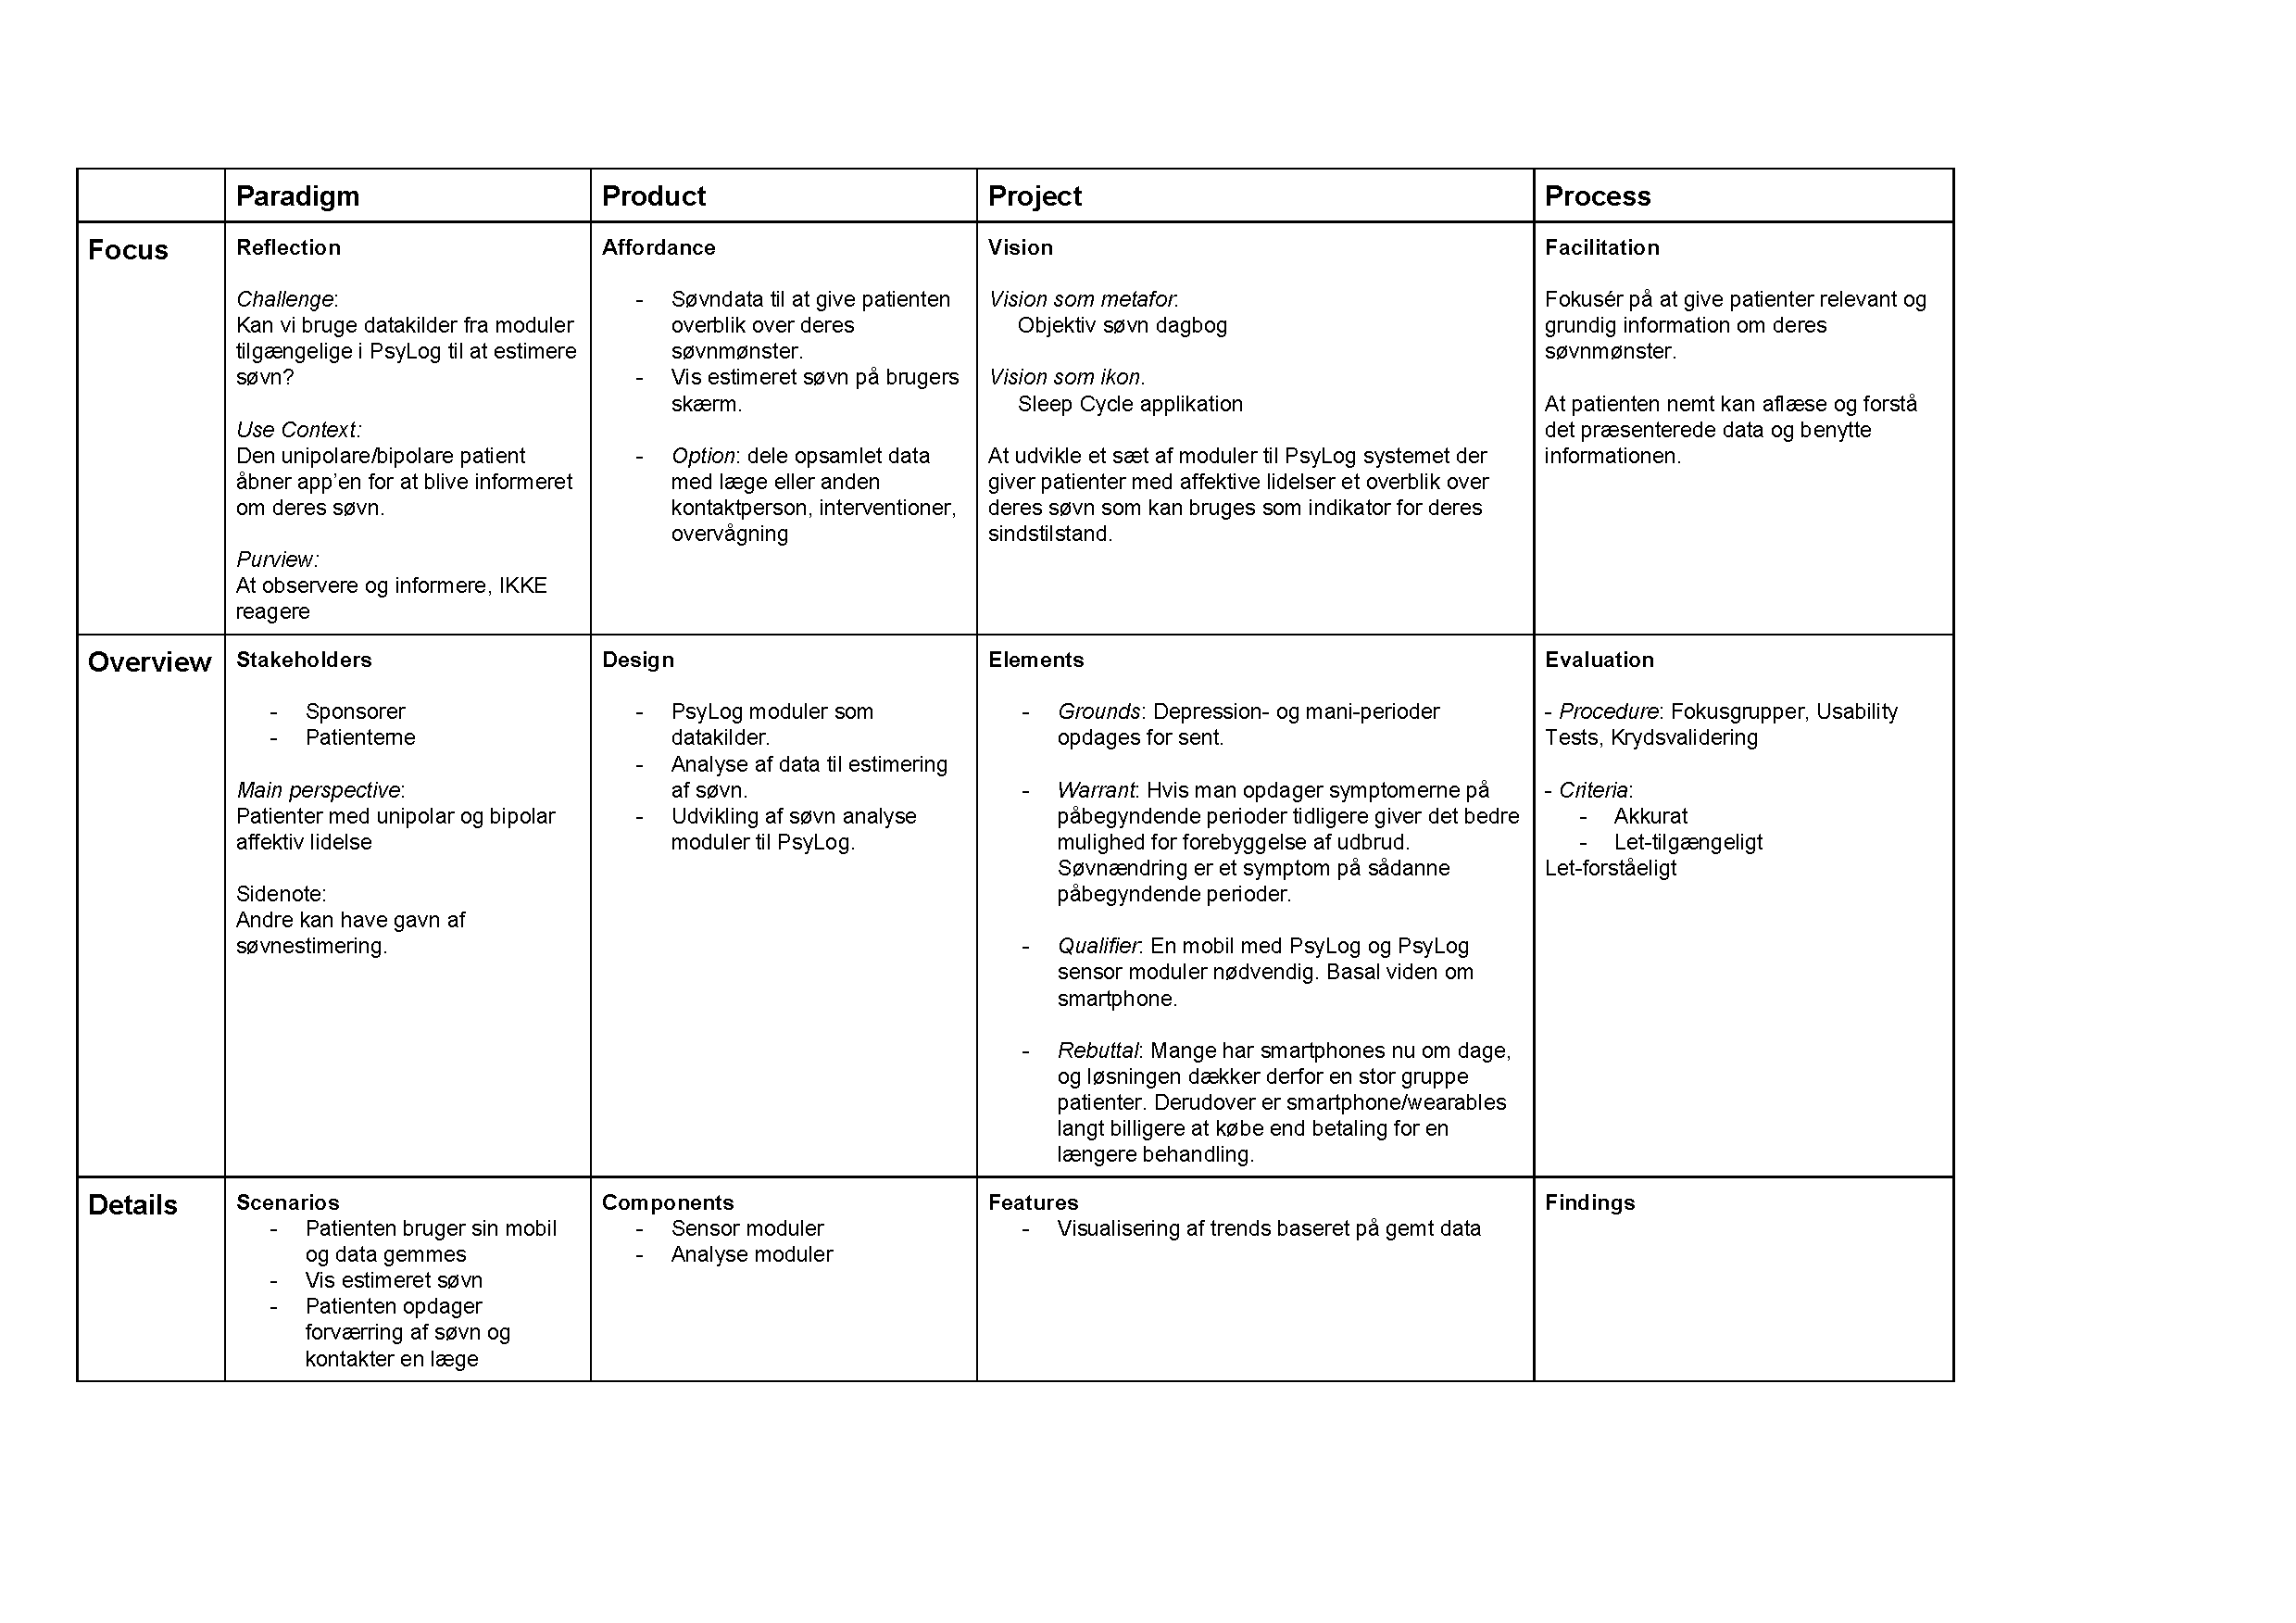
\includegraphics[scale = 0.65, angle =90,trim = 1cm 3cm 6cm 2cm, clip]{konfigurationstabel}
\caption{Konfigurations tabellen for systemet.}
\label{tab:konfigurationsTabel}
\end{figure}
\newpage
\section{Metodevalg}\label{sec:metodevalg}
For at kunne tage et valg omkring hvilket metoder, der skal vælges, gives et overblik over de metoder der er beskrevet i forskningen.
Disse valg skal evalueres ved hjælp af kriterier, og disse kriterier er baseret på idéen bag projektet, som er at systemet skal kunne lave målinger på patientens telefon uden at forstyrre og kunne lave analyser baseret på disse målinger. 

\begin{description}[style=nextline]
\item[Kriterie \#1: Undgå bruger intervention og måle søvn uden at forstyrre]
Dette ses som det helt centrale kriterie for vores løsning.
Grunden til dette er, at vi er interesseret i at registrere søvn for personer, der kan risikere at have en meget uforudsigelig søvn. 
Det kan være at patienten falder spontant i søvn på sofaen midt om dagen, og hvis personen, som krav for at kunne monitorere søvn, skal starte søvn modulet ville en sådan spontan søvn ikke blive registreret.
Derudover, blev der til fokusgruppeinterviewet \citep[Kapitel 1, Sektion 5]{misc:faellesrapp} lagt stor vægt på, at hvis en person er på vej imod en depression, vil enhver form for ekstra arbejde være en byrde man ville springe over.
Et system der kræver manuel aktivering for hver søvnperiode, vil derfor ikke være tilstrækkelig i sådanne scenarier, og er hvorfor et ikke forstyrrende system vægtes højt.

\item[Kriterie \#2: Kunne bruges af brugere i deres eget hjem]
Applikationen er tiltænkt som en personlig hjælper, hvor en patient kan holde øje med deres egen situation, især i den habituelle periode, for at holde øje med tegn på forværring.
Af denne grund er det centralt at systemet skal kunne bruges i eget hjem, og ikke være påkrævet hospitalsapparatur.
Dette hænger også sammen med, at man i den habituelle periode ikke er indlagt, men at man går hjemme.
Derudover er løsningen tiltænkt som en forebyggende applikation, hvorfor patienter i den habituelle periode er i fokus.

\item[Kriterie \#3: Være præcis]
For at man skal kunne stole på vores system, er det nødvendigt at det er tilstrækkelig præcist, så præcist at man ikke kommer med for mange forkerte estimater, da man risikerer at patienten vil undlade at bruge systemet. 
Derudover, hvis systemet er for upræcist har det intet formål, da idéen er at det skal kunne monitorere søvnen i højere grad end patienten selv.
Til at forøge præcisionen af metoden vil måling af søvnforstyrrelser være en fordel at have for den valgte løsning.
Måling af søvnforstyrrelser er dog ikke prioriteret særlig højt i forhold til andre ting, hvilket gør at det ikke er højst nødvendigt at kunne måle det.
\end{description}

\subsection{Opsummering af Metoder}
For at give et overblik over de forskellige metoder og teknikker opsummeres de i \cref{tab:opsummeringMetoder}.
Som en ekstra bemærkning til denne tabel er præcisionen baseret ud fra en antaget søvnlængde på otte timer. 

%tabellen skal rettes seriøst til, især quality delen skal være mere sammenlignelig
\begin{table}[h]
\begin{tabular}{|p{2cm}|p{2cm}|p{2cm}|p{2cm}|p{2cm}|p{2cm}|p{1.5cm}|}
\hline & Poly somnografi & ActiGrafi & Søvn Dagbog & Toss 'N' Turn søvn længde estimering & Best Effort Sleep  & Statistisk baseret\\ 
\hline Præcision & N/A (dog meget præcis) & 95\%+ & Subjektivt & 92\% & 92\% & 68\%\\ 
\hline Behøver eksperter & Ja & Nej & Nej & Nej & Nej & Nej \\ 
\hline Udstyr & Specialiseret udstyr & JawBone / FitBit & Ingen & Smartphone & Smartphone & Smart-phone \\ 
\hline Bruger intervention	& I laboratorie og meget udstyr på patient	& Monter udstyr / læg under hovedpude & Manuel registrering  & Oplærings-periode, derefter begrænset & Begrænset & Læg telefon i seng \\ 
\hline Metrikker & REM søvn, Meget præcist	& Let/Dyb søvn & Subjektivt & Længde, vækningsperioder og søvn kvalitet & Længde og vækningsperioder & Længde \\ 
\hline 
\end{tabular}
\caption{Opsummering af de forskellige metoder til søvnestimering.}
\label{tab:opsummeringMetoder}
\end{table}

Som det kan ses ud fra \cref{tab:opsummeringMetoder}, så har de forskellige metoder varierende styrker og svagheder, Toss 'N' Turn's søvn længde estimering og Best Effort Sleep har dog samme kvaliteter.
For at beslutte hvilke metoder der skal arbejdes videre med, skal vi udover at forholde os til de opstillede kriterier, også vurdere hvilke metoder vi har mulighed for at lave, med det udstyr og de konkrete ressourcer vi har til rådighed.
Da polysomnografi kræver en ekspert og store mængder specialiseret udstyr, er denne ikke fornuftig at se videre på.
ActiGraf kræver en wearable som dataindsamlings modul, hvilket vi ikke har, så derfor kigges der ikke videre på den, men hvis sådanne wearables var til rådighed, ville denne metode kunne give meget gode resultater.

En søvndagbog kunne godt være passende, dog er der det problem at det er subjektivt så patienten kan komme til at give ukorrekt information, hvilket vil virke forstyrrende for et program der skal finde trends.
Derudover, er der en risiko for at patienterne ikke udfylder deres søvndagbog hvis de er i en depressions- eller maniperiode.

Dette efterlader os med tre tilbageværende metoder, Toss 'N' Turn, Best Effort Sleep (BES) og den statistisk baseret tilgang.
Af disse har BES og Toss 'N' Turn bedst præcision, hvor BES kan køre stort set uden at involvere brugeren, hvorimod Toss 'N' Turn har brug for en læringsperiode hvorefter brugeren ikke involveres længere.
Den statistisk baserede metode kræver involvering af brugeren, hvilket er at telefonen skal ligge i patientens seng, på det punkt er det en god middelvej, men den har væsentlig lavere præcision end de to andre.

Se \cref{tab:soevnMetodeKriterier} for hvordan Toss 'N' Turn, Best Effort Sleep og den statistisk baseret metode opfylder kriterierne.

\begin{table}
\begin{tabular}{|p{4cm}|p{3cm}|p{3cm}|p{3cm}|}
	\hline  ~ & \#1: Undgå bruger intervention og måle søvn uden at forstyrre & \#2: Kunne bruges af brugere i deres eget hjem & \#3: Være præcis \\ 
	\hline Toss 'N' Turn &  & \checkmark & \checkmark \\ 
	\hline Best Effort Sleep & \checkmark & \checkmark & \checkmark \\ 
	\hline Statistisk baseret &  & \checkmark &  \\ 
	\hline 
\end{tabular}
\caption{Hvordan de 3 forskellige metoder overholder kriterierne.}
\label{tab:soevnMetodeKriterier}
\end{table}

Ud fra dette skal der så udvælges en metode der skal fokuseres på. 
Netop fordi vi gerne vil have så lidt krav til bruger intervention som muligt, vil vi kraftigt foretrække en metode som ikke kræver noget af brugeren, hvilket kan være Best Effort Sleep (BES) metoden, dog kræver Toss 'N' Turn ikke meget bruger intervention da det er kun i læringsperioden at det er påkrævet.
For både BES og Toss 'N' Turn har det ikke været muligt for os at finde en præcis beskrivelse af hvordan man fortolker og kombinerer de forskellige datakilder, så det skal vi selv genskabe.
Dog ved vi ud fra artiklerne at det er muligt at gøre, hvilket betyder at de begge er reelle valg. 
BES har dog også det problem at den kun kan beregne søvnlængden og ikke søvn kvalitet, som mange mener også er ganske relevant for adfærdsændringer, da et af det beskrivende kriterier for at være i en depressions periode er at ens søvn er ustabil eller af dårlig kvalitet. 
Manglen på denne egenskab gør at BES alene ikke er beskrivende nok til at dække alt, hvilket vil sige at hvis man skal måle søvn kvalitet skal man opsøge andre metoder.

Da der ikke er meget tid til at lave noget udtømmende, udvælges en metode, der skal arbejdes på som et proof of concept, hvor så udviklingen af andre metoder kan forsættes senere.
Vores design af platform sikrer en høj modularitet og fleksibilitet, hvorfor det ikke forekommer svært at ændre søvnestimeringsmetode på et senere stadie.

Valget falder på en implementering af Best Effort Sleep selvom den ikke måler søvnkvalitet.
Hvis der havde været mere tid til rådighed, ville valget med alt sandsynlighed være faldet på en implementering af Toss 'N' Turn, da denne som tidligere nævnt også har mulighed for at vurdere søvn kvaliteten.
Grunden til at BES vælges i første omgang er at denne vurderes knap så kompleks som Toss 'N' Turn og passer derfor bedre til en proof of concept løsning.

Det at kvalitetsvurderingen også kommer med vil kunne tilføje et ekstra lag til vurderingen af folks søvn, hvilket er meget vigtigt, da det godt kan være man ligger i sin seng og forsøger at sove i omkring 8 timer, men hvis man ikke sover sammenhængende i mere end for eksempel 45 minutter, er det ikke et godt tegn.
Dette ekstra vurderingselement er meget vigtigt i den store sammenhæng, da det er essentielt i den proces det er at vurdere om en person har en depression. 



\chapter{Implementering af Søvnestimering}
% Fortæl om at nu har vi forskning --- masse nyttig viden
Forarbejde for søvnestimering er foretaget og beskrevet i \cref{chap:forarbejdsoevn}.
Ud fra det er der tilegnet en masse nyttig information, samt udarbejdet en konfigurationstabel for at give et overblik over udviklingen af produktet.
I forskningen af søvnestimeringsmetoder er der fundet en række forskellige måder at estimere søvn på, men desværre har vi ikke kunne finde løsninger hvis implementering er offentlig tilgængeligt.
Af den grund er vi nødsaget til at implementere en løsning selv, hvilket er beskrevet i dette kapitel.
Dog har forskningen af søvnestimeringsmetoder givet nyttig viden om redskaber indenfor søvnestimering, hvilket er beskrevet først i dette kapitel.
Derudover beskrives overvejelser omkring snorken, der er vigtigt at have i mente når der tales om søvn.
Efter dette beskrives konstruktionen af en proof of concept metode der benytter sig af de nævnte redskaber.
Dette inkluderer en beskrivelse af forsøgsopstillingen, en systematisk gennemgang af metoden inklusiv et eksempel, samt en diskussion af hvordan man bør verificere metoden, for at sikre at den har den fornødne præcision.
Efter denne gennemgang følger en diskussion af videre arbejde der bør foretages mht. produktudviklingen.



% Desværre er det ikke i public space, så vi bliver nødt til at udvikle vores eget

% Vi kan stadig drage fordel af den viden vi har fået

% Så vi kommer med opsummering af nogle af de gode ting derfra

% Beskrivelse af vores model og hvad man kan gøre for at verificere den

% Beskrivelse af videre arbejde
\section{Platform}
Som et led i arbejdet blev der udviklet en platform kaldet PsyLog \citep{misc:faellesrapp}, som moduler kan hægte sig på.
Platformen er nyttig, da den tilbyder en række dataindsamlingsmoduler samt lagerplads, som ens modul kan benytte sig af.
Derudover, kan ens modul indgå i en større software pakke, hvor andre moduler kan drage nytte af ens estimater.

PsyLog er en platform, der er konstrueret til at være modulær og fleksibel.
Til at understøtte denne funktionalitet tilbyder platformen en database, hvor moduler kan lagre data og læse data lagret fra andre moduler.
Det eneste krav til hvert modul er, at de skal implementere en service, som kan startes af platformen, og at de har en JSON beskrivelse.
JSON beskrivelsen indeholder tabeller til lagring af data, moduler de afhænger af, samt om modulet skal skemalægges eller om det bare skal køre hele tiden.
Hvis man har dette specificeret, sørger PsyLog platformen for resten, det vil sige start af modulet samt sikre lagerplads som modulet kan skrive til og læse fra.

\subsection{Dataindsamlingsmoduler}
Som et led i udviklingen af PsyLog platformen er der blevet udviklet en række dataindsamlingsmoduler \citep{misc:faellesrapp}.
I \cref{sec:metodevalg} har vi erfaret at fælles for metoderne er at de alle kigger på om smartphonen er stationær og om der er stilhed. 
Til stilhed kan vi benytte det allerede udviklede amplitude-modul, og til at se om en smartphone er stationær kan vi benytte det allerede udviklede accelerationsmodul.
Vi har altså dataindsamlingsmoduler til disse typer data allerede, og kan med fordel benytte dem i videre implementering.
Derudover, nævner hver kilde flere moduler, der er specifikke for deres løsning, hvoraf flere er udviklet.
PsyLog platformen har den fordel, at den er fleksibel og modulær, hvilket gør at hvis man skulle mangle et dataindsamlingsmodul for en given datatype kan et sådant modul sikkert nemt udvikles og benyttes.
Metrikker for vores datatyper er hvad der er beskrevet i \cref{sec:metrikker}.
\section{Redskaber}\label{sec:redskaber}
\ivan{Hvad er et redskab?}
\winde{Ivans rettelser her til!}
%Noget meta fiks med hvilke redskaber og erfaringer vi kan tage med os til udvikling af løsning
Med forskningen af søvn foretaget har vi fundet diverse redskaber, der er værd at have i mente ved implementeringen af en søvnestimeringsmetode.
Gennemgangen af disse redskaber tjener det formål at skabe overblik, over hvad man kan benytte i denne implementering.
Metoderne bygger på erfaringer oplyst af kilderne, samt teknikker der bygger på egen erfaring, men regnes for brugbare i denne sammenhæng.

\begin{description}[style=nextline]
% PsyLog - herunder dataindsamlingsmoduler
\item[PsyLog]\ivan{Overvej at lave et separat afsnit med Psylog og Dataindsamlingsmoduler}
PsyLog er en platform, der er konstrueret til at være modulær og fleksibel.
Til at understøtte denne funktionalitet tilbyder platformen en database, hvor moduler kan lagre data og læse data lagret fra andre moduler.
Det eneste krav til hvert modul er, at de skal implementere en service, som kan startes af platformen, og at de har en JSON beskrivelse.
JSON beskrivelsen indeholder tabeller til lagring af data, moduler de afhænger af, samt om modulet skal skemalægges eller om det bare skal køre hele tiden.
Hvis man har dette specificeret, sørger PsyLog platformen for resten, det vil sige start af modulet samt sikre lagerplads som modulet kan skrive til og læse fra.
Derudover, kan ens modul så indgå i en større software pakke, hvor andre moduler kan drage nytte af ens estimater.

\item[Dataindsamlingsmoduler]\ivan{Overvej at lave et separat afsnit med Psylog og Dataindsamlingsmoduler}
Som et led i udviklingen af PsyLog platformen er der blevet udviklet en række dataindsamlingsmoduler \citep{misc:faellesrapp}.
I \cref{sec:metodevalg} har vi erfaret at fælles for metoderne er at de alle kigger på om smartphonen er stationær og om der er stilhed. 
Til stilhed kan vi benytte det allerede udviklede amplitude-modul, og til at se om en smartphone er stationær kan vi benytte det allerede udviklede accelerationsmodul.
Vi har altså dataindsamlingsmoduler til disse typer data allerede, og kan med fordel benytte dem i videre implementering.
Derudover, nævner hver kilde flere moduler, der er specifikke for deres løsning, hvoraf flere er udviklet.
PsyLog platformen har den fordel, at den er fleksibel og modulær, hvilket gør at hvis man skulle mangle et dataindsamlingsmodul for en given datatype kan et sådant modul sikkert nemt udvikles og benyttes.
Metrikker for vores datatyper er hvad der er beskrevet i \cref{sec:metrikker}.

\item[Vægtet gennemsnit]
Ud fra \citet{6563918} blev der understreget hvorledes et vægtet gennemsnit kan benyttes.
Idéen er at hver sensor kilde kan benyttes som en svag indikator på søvnlængde.
Imidlertid bør man ikke stole på udelukkende en kilde, da den søvnlængde man estimerer kan variere meget ved forskellig brug af smartphonen.
For så at have et mere sikkert estimat for søvnlængde, foretager man et såkaldt vægtet gennemsnit af hvert estimat, hvor kilder, der er mere sikre end andre får tillagt en større vægtning.

\item[Eksponentielt glidende gennemsnit]
Da man oplever støj på de forskellige sensorkilder kan man med fordel benytte et eksponentielt glidende gennemsnit.
Basalt set er et eksponentielt glidende gennemsnit en måde at udjævne tilfældige udsving i en serie af punkter.
Eksempelvis ved accelerations målinger oplever vi enkelte spikes på grund af støj, og disse kan udjævnes ved hjælp af det eksponentielle glidende gennemsnit.

\item[Krydsvalidering]
Når man udvikler sin estimeringsmetode skal man have en teknik til at estimere om ens model er tilpas præcis.
Problemet er at hvis man lærer på sit testdata og derefter tester på dette, risikerer man hvad der kaldes for overfitting.
Overfitting er hvor man tilpasser sin model så det virker godt på ens testdata, men ikke særligt godt på fremtidige datasæt.
Til at forhindre dette kan man foretage krydsvalidering
Ved krydsvalidering splitter man sit testdata op i en række delmængder.
Man foretager så analysen på en delmængde og validerer sin analyse på de resterende delmængder af datasæt.
For så at undgå overfitting afprøver man med forskellige partitioner af datasættet, og hvor ens præcision er estimeret som gennemsnittet af resultaterne af de datasæt man tester på.

% Stilstand
% Chen et al og andre
\end{description}
\subsection{Snorken}\label{section:snorken}
\ivan{Overvej placering af dette afnist, eller at forberede denne diskussion f.eks. i starten af kapitlet}
Snorken er en åbenlys faktor, der skal tages højde for når man skal opdage søvn ved hjælp af sensorer, idet en af de primære sensorer, som bruges til at bestemme om en person sover er lyd.
Hvis lyden gentagne gange optager snorken, vil den nuværende sandsynlighedsudregningen for denne sensor falde hver eneste gang snorken bliver optaget, og dette er helt klart et problem, som skal arbejdes videre på.

Et eksempel kan ses i \cref{fig:snorke-vs-ikkesnorken} hvor vi sammenligner en person som vi ved snorker mod en som ikke snorker.

\begin{figure}[h]
\begin{subfigure}{0.49\textwidth}
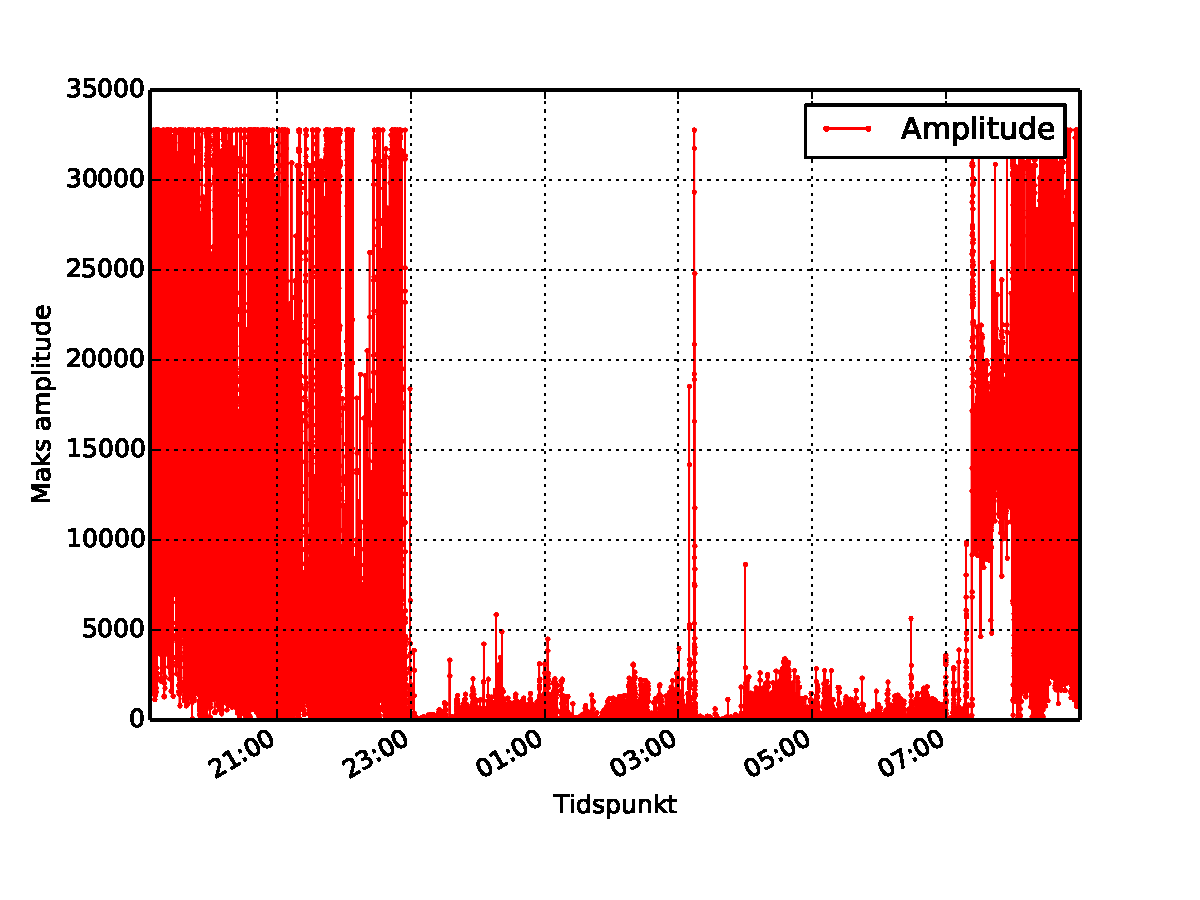
\includegraphics[width=1\textwidth,trim = 0cm 1cm 1cm 1cm,clip]{amplitude-plot-snorken}
\caption{Person der snorker}
\label{fig:person-snorker}
\end{subfigure}
\begin{subfigure}{0.49\textwidth}
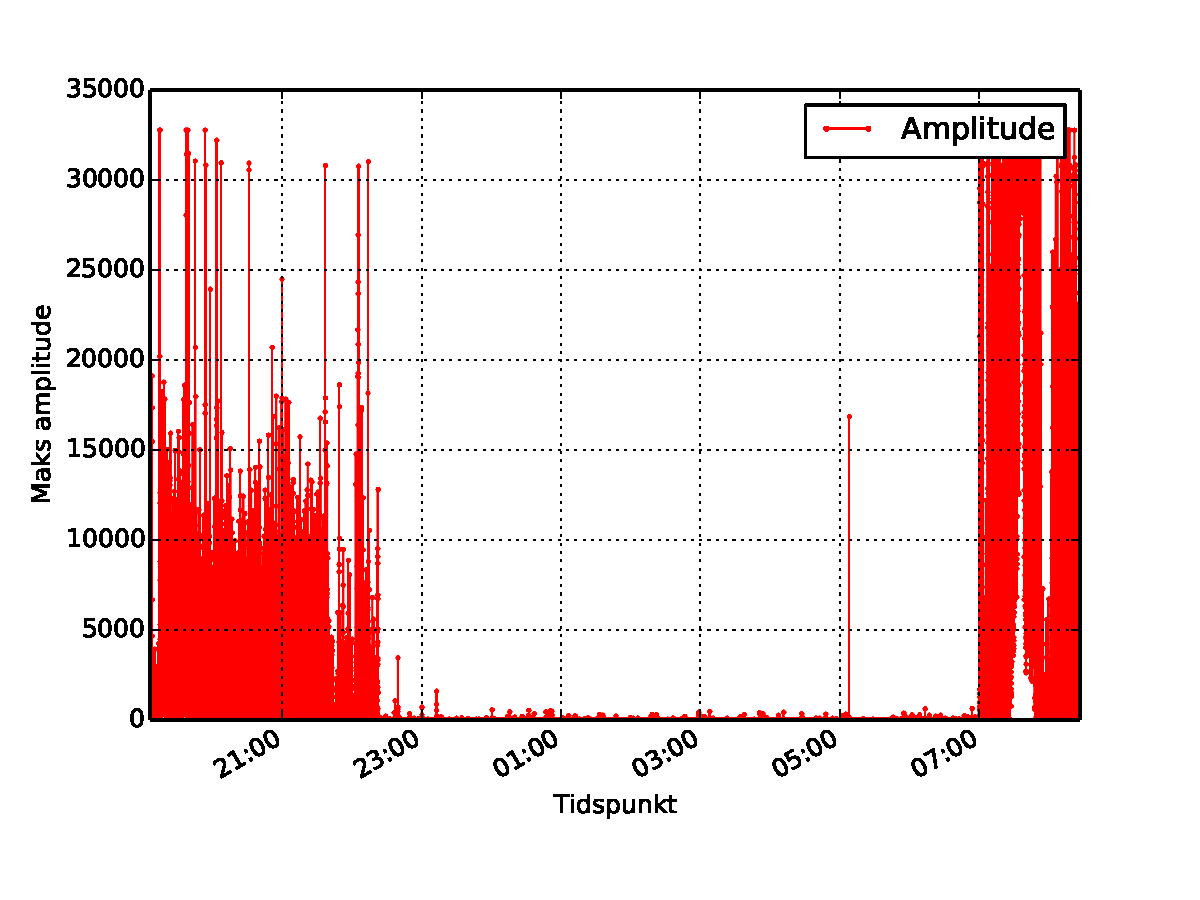
\includegraphics[width=1\textwidth,trim = 0cm 1cm 1cm 1cm,clip]{amplitude-plot-ingen-snorken}
\caption{Person der ikke snorker}
\label{fig:person-ikke-snorker}
\end{subfigure}
\caption{Person vi ved snorker og person vi ved ikke snorker}
\label{fig:snorke-vs-ikkesnorken}
\end{figure}

Hvis man ser på grafen med snorken, \cref{fig:person-snorker}, kan man se at amplituden er mere irregulær i søvn perioden i forhold til grafen i \cref{fig:person-ikke-snorker}. 
En simpel løsning på hvordan man kunne ignorere snorken i sandsynlighedsestimeringen vil være at sætte amplitude tærskelværdien op på et højere niveau, hvilket baseret på graferne kan være 5000. 
Tærskelværdien sætter grænsen for hvilken amplitude vi betragter som stilhed eller ej.
Men dette skal være baseret på hvor højt personen snorker og skal derfor være dynamisk, hvilket kan gøre at denne løsning ikke er optimal. 
Derudover, kan man ikke garantere at der ikke findes personer, der snorker lige så højt som når de snakker.
Andre metoder på at registrere søvn er derfor undersøgt.

Ud fra artiklerne \citet{Dafna2013}, \citet{Calabrese20111101} og \citet{7051338} dannes der et grundlag for hvordan snorken kan registreres.

\citet{Dafna2013} gør brug af et system til at inddele snorken og andre akustiske hændelser gennem et søvnforløb ved brug af lyd data, der blev optaget med en mikrofon ved en polysomnigrafisk undersøgelse. 
De endte med et meget præcist system, som kunne adskille snorken og andre akustiske hændelser med ~98\% nøjagtighed.
Denne metode kan tilpasses ind i vores system på den måde, at hvis snorken kan opdages har den ikke en negativ indflydelse, men derimod have en positiv indflydelse på sandsynlighedsberegningen af søvn. 
De bruger lyd data og ikke bare amplituden, så det vil være nødvendigt at undersøge om systemet også kan fungere ved brug af amplitude.
Grunden til at vi valgte at bruge amplituden, er at alt data gemmes og intet slettes, hvis løsningen ændres således at data analyseres løbende og slettes efterfølgende kan lyd data godt bruges, hvilket gør at vi undgår problemet med privatlivets fred.

\citet{Calabrese20111101} foreslår et system, der skal bruges til diagnosticering af søvnapnø ved hjælp af optaget lyd.
Dog blev der kun implementeret en prototype af systemet og den er derfor ikke blevet evalueret ordenligt endnu. 
Idéen er at man bruger analyser såsom 'Fast Fourier Transform' og 'Power Spectrum' til at finde tidspunkter, hvor personen har snorket baseret på optaget lyd. 
Denne metode sår tvivl ved løsningen om blot at indsamle maks amplitude, da om nødvendigt skal lydindsamlingen ændres til et sliding window.
Det vil sige, hvor vi samler det rå lyddata fra mikrofonen, men sletter lyddata efter en analyse er foretaget, således at privatlivs kriteriet stadig opfyldes.
Dette er en mulighed et modul kan benytte sig af, og bør udforskes med videre arbejde.

\citet{7051338} udvikler et system, der kan registrer snorken ud fra lydoptagelser.
Denne metode bruger machine learning til at udvikle en model der detektere hvornår folk sover.
Metoden der er udviklet gør brug af en \textit{K}-Nearest Neighbour classifier.
Derudover, kræver metoden ligesom den forrige at vi optager lyd i stedet for bare at se på amplituden.
I modsætning til \citet{Calabrese20111101}, fokuseres der på at registre snorken, hvilket også kvalificerer denne metode som en oplagt kandidat til videre udforskning.

Hvis man vælger at arbejde videre med en af disse metoder til at detektere snorken, har det også andre anvendelsesmuligheder end at fjerne støj fra vores estimering.
Hvis en af metoderne registrerer at man snorker, kan man sige at det uden tvivl betyder at en person sover, og så kan den sandsynlighedsvurdering der ellers havde været på det tidspunkt blive overskrevet med 100\%.
Dette er en meget relevant ting at bruge snorke registrering til, da man så kunne betragte snorken som en styrke ved estimering fremfor bare støj.
\section{Proof of Concept}
Baseret på den viden der er blevet indsamlet, laves der er et proof of concept til søvndelen af projektet.
Denne implementering er beskrevet herunder.
Grunden til at der kun laves et proof of concept og ikke et fuldstændigt færdigt system er, at der ikke er nok tid til at gøre det helt færdigt. 
Ydermere, vil et helt færdigt system påkræve testning hos målgruppen, og dette er der ikke er tid nok til at udføre. 

Denne sektion om proof of concept beskriver valg af nødvendig sensor data, hvordan søvnestimering udføres på data, og hvordan søvnestimeringerne for de forskellige sensorer kombineres og hvordan denne estimeringen skal aggregeres til individuelle perioder af søvn.

% Manglende resourcer
% Time constraints.
% Ingen test mulig(Kræver tilladelser, og system ikke færdig)

Som et proof of concept er der blevet valgt at implementere en enkelt metode til at afgøre hvorvidt man sover eller ej.
Metoden er baseret på redskaberne beskrevet i \cref{sec:redskaber}, hvor der som start til dataindsamling ses på amplitude og acceleration.
Grunden til at vi starter med disse to datakilder er fordi \citet{6563918} erfarede, at det er de langt væsentligste datakilder, hvilket også er beskrevet i \cref{sec:BES}.

Disse to datakilder kombineres til en enkelt model, der skal kunne afgøre hvorvidt man sover eller ej.
Med mere tid vil de andre nævnte datakilder også blive fokuseret på.

For at have en regelmæssig måde at indsamle data, der ligger til grund for implementeringen af det efterfølgende søvnestimeringsmetode, er det nødvendigt at have forsøgsopstillingen beskrevet, hvorfor denne følger herefter.
\subsection{Forsøgsopstilling}
%Disposition:
%Billede af opstilling
%Bare tage med hjem og sove
%Flere forsøg og systematisk tilgang kunne være brugt og skulle gøres hvis det ikke bare var proof of concept.
For at forsøget fortages på samme måde hver gang, så det indsamlede data er sammenligneligt, valgte vi at lave en forsøgsopstilling.
\begin{figure}[h]
	\centering
	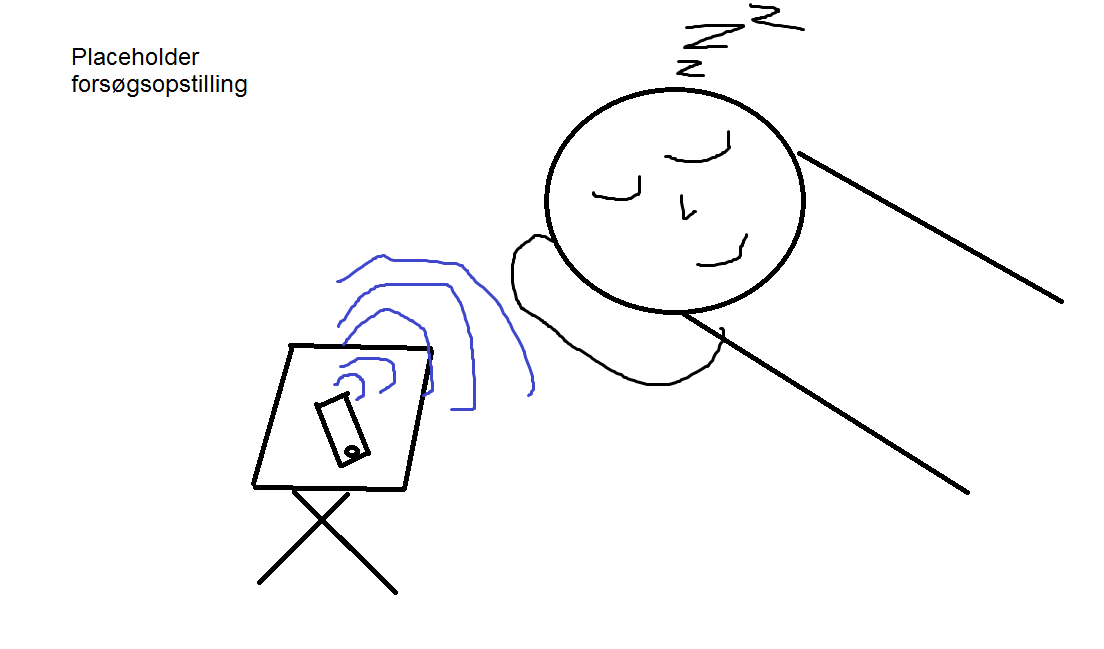
\includegraphics[scale=0.5,trim = 0cm 0cm 5cm 10cm, clip]{forsoegsopstilling}
	\caption{Forsøgsopstilling. Sovende person med smartphonen på natbordet.}
	\label{fig:forsoegopstillings}
\end{figure}

Forsøgsopstillingen kan ses i \cref{fig:forsoegopstillings} der illustrerer hvordan smartphonen ligger på natbordet og indsamler data.
Idéen er at det eneste krav til indsamlingen er, at den skal ligge på et bord i soveværelset når der soves, ellers står det en frit om man går med smartphonen i lommen, lægger den på skrivebordet eller andet. 
Dette valg er foretaget i henhold til vores kriterie om at udvikle et system der kan måle søvn uden at forstyrre.

Indsamlingen af data foregik ved at vi installerede de fornødne moduler på egen smartphone, Tog smartphonen med hjem, så data fra en eller flere dage kunne indsamles.
Vi loggede fra vi gik i seng til vi stod op, hvilket skulle bruges til at afgøre nøjagtigheden af vores estimat.

Til at validere vores model har vi foreslået krydsvalidering beskrevet i \cref{sec:redskaber}, hvilket også bør gøres med mere tid, men da dette er et proof of concept er den nuværende opstilling tilfredsstillende.
Ved videre arbejde bør en mere systematisk tilgang med den nævnte krydsvalidering benyttes, hvilket er beskrevet videre i \cref{sec:verisoevn}.

\subsection{Sensor Data}
For at have en bedre indsigt i hvordan vi kan bruge accelerations- og amplitude-data blev disse plottet over en dag inklusiv søvn.
Dette kan ses i \cref{fig:accplot} og \cref{fig:amplplot}.

\begin{figure}[h]
	\centering
	%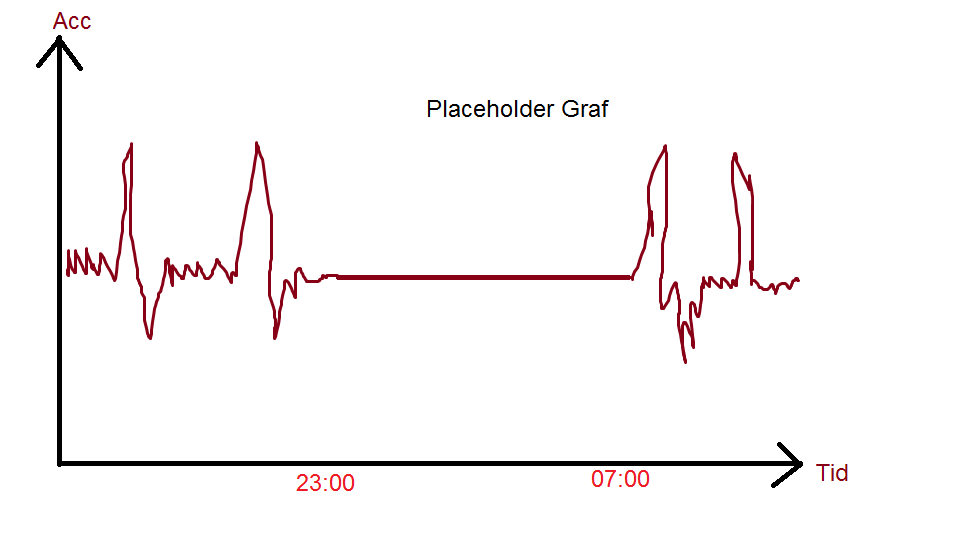
\includegraphics[scale=0.5]{acc-placeholder}
	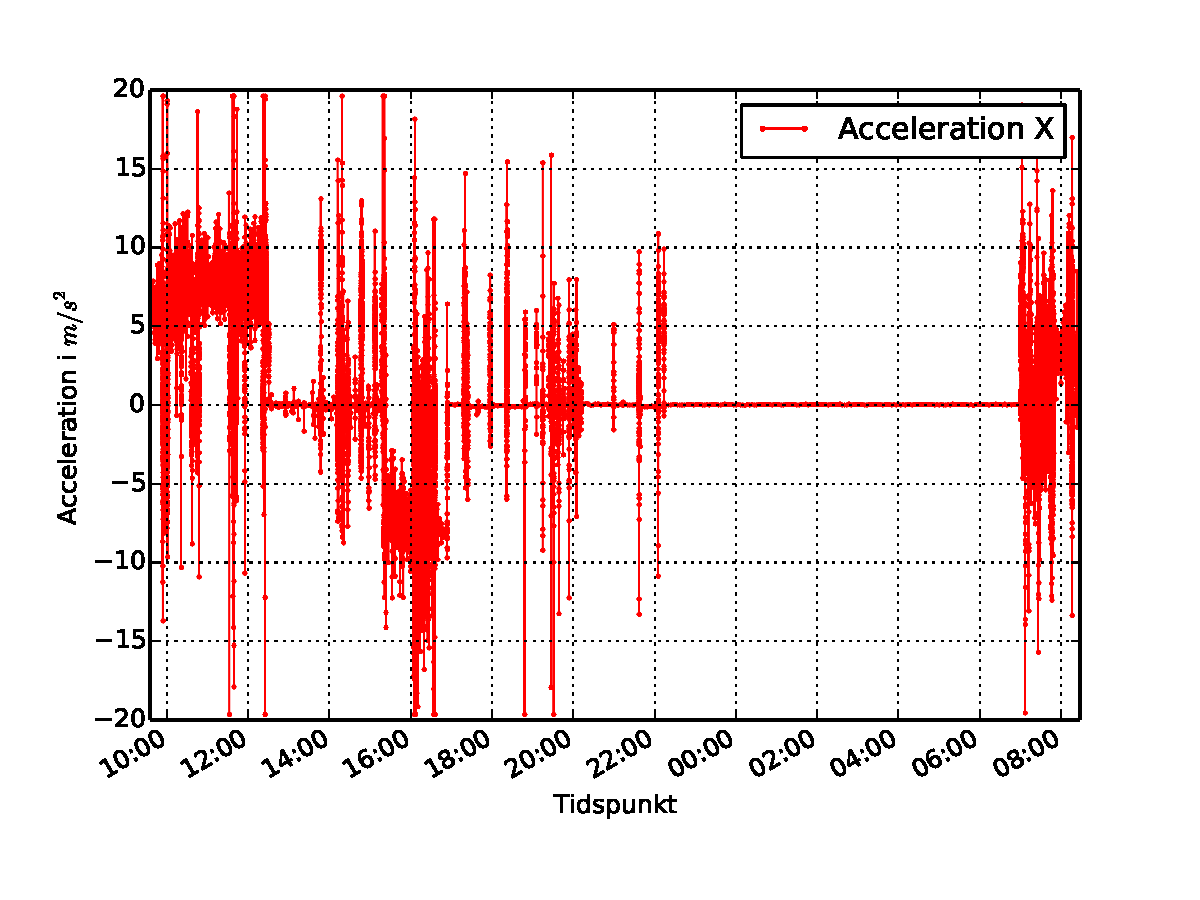
\includegraphics[scale=0.75]{acceleration-plot}
	\caption{Accelerationsplot, hvor der blev sovet fra ca. 22:00 til 07:00 næste dag.  Et punkt svarer til en måleværdi.}\label{fig:accplot}
\end{figure}

Ses der på accelerationsdata i \cref{fig:accplot} indikerer det tydeligt når smartphonen har været i bevægelse og når smartphonen ikke har været i bevægelse.
Dette skyldes at et accelerometer er god til at registrere bevægelse, da acceleration er ændring i hastighed.
Det viser sig at plottet fint indikerer når man er vågen, hvilket er forårsaget af at testpersonen har gået med sin smartphone i lommen.
Dog kan man ved stilstand ikke vide sig sikker på om det er fordi man sover, eller blot fordi man har lagt sin smartphone fra sig.

Ved stilstand i en længere periode, kan man estimere sandsynligheden for at denne stilstand er at brugeren sover. 
Derudover kan andre sensor inputs hjælpe til at klargøre denne tvivl, der ikke er begrænset til at man skal have smartphonen i lommen.
Et eksempel på en sådan kilde er mikrofonen, som vi kan bruge til at måle maks amplitude.
At vi kun måler maks amplitude sikrer at personfølsomme oplysninger ikke indsamles, da man ikke kan genskabe en samtale, men blot har maks amplitude lagret for hvert sekund.

\begin{figure}[h]
	\centering
	%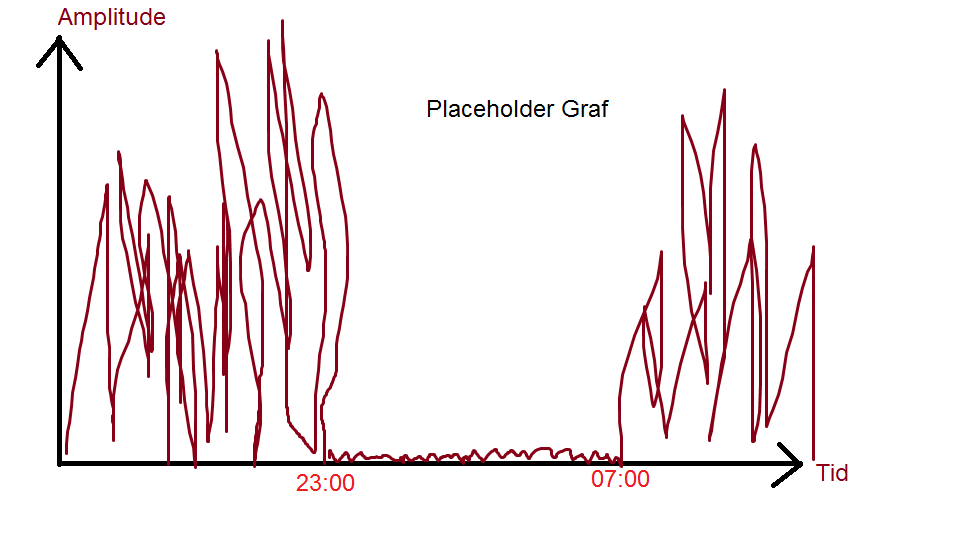
\includegraphics[scale=0.5]{ampl-placeholder}
	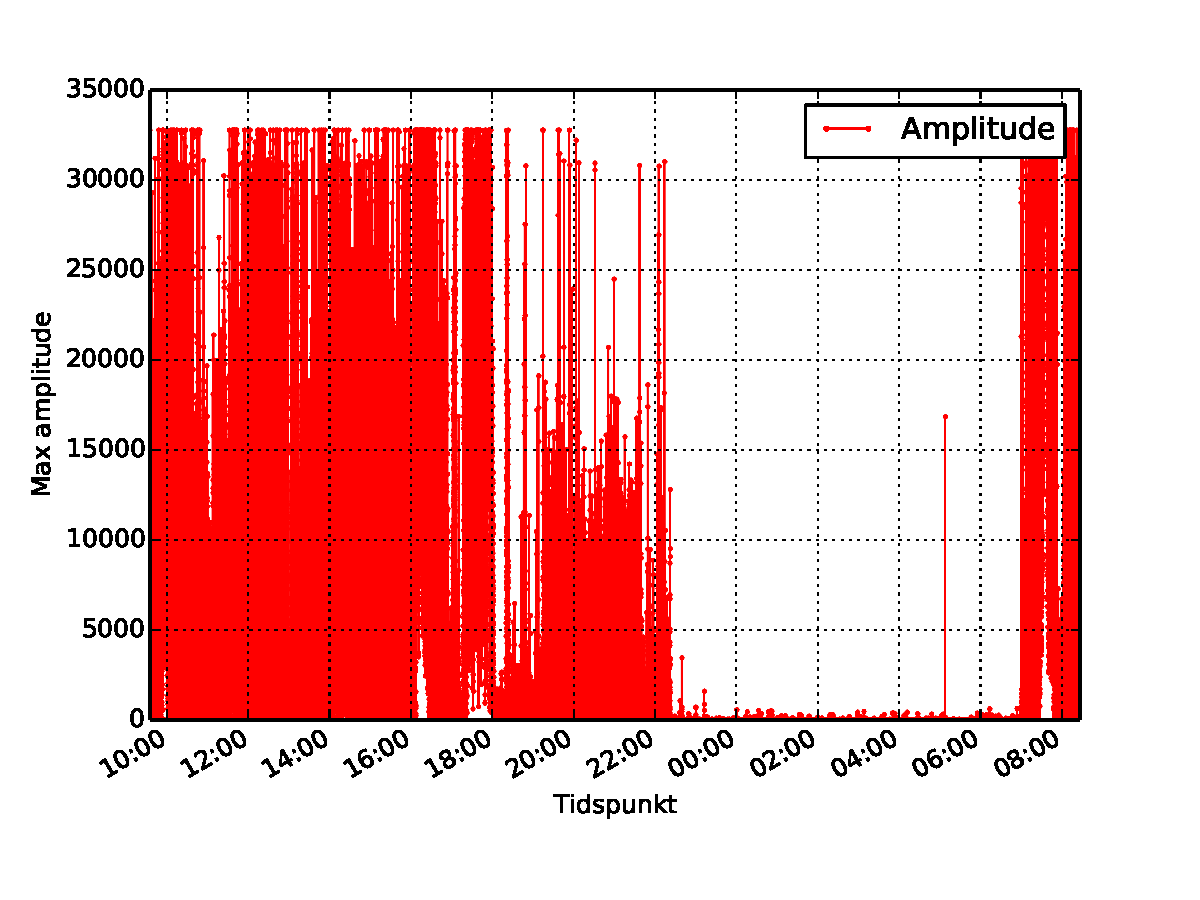
\includegraphics[scale=0.75]{amplitude-plot}
	\caption{Amplitudeplot, hvor der blev sovet fra ca. 22:00 til 07:00 næste dag. Et punkt svarer til en måleværdi.}\label{fig:amplplot}
\end{figure}

Idéen bag at bruge maks amplituden er at man larmer væsentligt mere når man er vågen end når man sover.
Dette passer fint med de loggede data der er plottet i \cref{fig:amplplot}.
Dog har denne antagelse også begrænsninger.
Eksempelvis kan det være at man er en stille person, snorker meget eller også kan personen bo i et meget larmende område.
Alligevel regner vi med at amplituden stadig kan bruges, da man så muligvis kan finde et mønster når man snorker til at styrke modellen, hvilket er tidligere diskuteret i \cref{section:snorken}.
Derudover, er det så et spørgsmål om hvor stor vægt man skal tillægge de enkelte sensorkilder, og er noget der bør trænes til det enkelte individ, for at opnå en model der passer til individets personlighed.
Hvordan dette gøres bør overvejes ved videreudvikling, men til dette proof of concept kan man som en start bruge fastsatte statiske vægte, hvilket er diskuteret i \cref{subsec:sensorvaegtsoevn}.

\subsection{Søvnestimerings model}
Ud fra observeret data etablerer vi nogle antagelser som vi går ud fra også holder til fremtidigt data.
Disse er at når man observerer en handling om det er acceleration eller amplitude, kan vi med stor sikkerhed sige at man ikke sover.
Modsat hænger sandsynligheden for at man sover sammen med længden af stilstand.

Dette får os til at lave en model der bygger på disse to antagelser, hvilket er gjort for at skabe jordforbindelse.
Dette betyder at vi udvikler en metode, for at bekræfte at det kan blive implementeret til en smartphonen med den valgte platform.
Som nævnt har vi ikke kunnet finde passende metoder, der er offentligt tilgængeligt, hvorfor vi bliver nødt til at udvikle vores egen metode.

Vores model går på en sliding window tilgang, hvor den centrale del er at registrere stilstand med acceleration og amplitude.
Konceptet om stilstand er taget fra \citet{6563918} angående Best Effort Sleep, og er hvilken model vores metode tager primært udgangspunkt i.
Toss 'N' Turns tilgang, hvor man ser på 10-minutters vinduer med data til at afgøre søvn eller ikke søvn er et alternativ.
Dette alternativ blev dog valgt fra i første omgang, som nævnt i \cref{subsec:summametoder}, da stilstandsbestemmelsen vurderedes mindre komplekst og egnede sig derfor bedre til en proof of concept løsning.
Med mere tid kunne Toss 'N' Turn tilgangen blive forsøgt implementeret.

\subsubsection{Stilstands-bestemmelse}
Som udgangspunkt for vores udkast til en søvnestimeringsmodel afgøres der hvornår der er stilstand.
Dette gøres forskelligt for acceleration og amplitude data, men tager udgangspunkt i det loggede data.
For at sikre at støj ikke påvirker resultatet kan der bruges forskellige strategier i brug. 
For eksempel hvis man ændrer drastisk på hvor ofte mikrofonen optager amplitude til f.eks. at optage hvert tiende sekund, vil dette resultere i færre datapunkter og hvis dette gøres indfanges der mindre støj.
Dog kan dette også håndteres på andre måder, for eksempel ved et glidende gennemsnit, nævnt i \cref{sec:redskaber}, udført på indsamlede data, men hvis man kan undgå at bearbejde data ved at indsamle mindre vil dette være en fordel.

Vi valgte at gøre det ved hjælp af et glidende gennemsnit fordi hvis man ændrer på hvor ofte sensorerne indsamler data, vil det muligvis have en påvirkning på andre moduler.
Derudover, hvis man skal indsamle færre datapunkter, er det vigtigt at vide hvor ofte man skal indsamle disse datapunkter for at undgå støj.
Dette vil dog kræve at man udfører eksperimenter for at finde ud af hvor ofte man skal indsamle datapunkter.
Dermed virkede det glidende gennemsnit til at være en simplere løsning til vores problem.

Hvis vi ser på \cref{fig:accplot}, der er et plot for accelerationsdata, kan vi se stilstand for punkterne mellem 22:00 og 07:00.
Øvelsen består i at have en metode der kan afgøre at disse punkter er i stilstand.
Dette gøres ved at for et givent punkt at se om de 5 tidligere målinger ikke afviger fra en given fastsat grænse fra punktet i betragtning i x, y og z aksen.
Pseudokode til at tjekke dette kan ses i \cref{lst:pseudoStationary}.

\begin{lstlisting}[caption={Pseudo kode for at tjekke om et punkt er i stilstand.}, label={lst:pseudoStationary}]
isStationary(accToConsider : AccelerationReading, previousPoints : Collection of AccelerationReadings) : boolean
   foreach acc in previousPoints
      if outOfThreshold(accToConsider, acc)
         return false
   return true
\end{lstlisting}

Hvis der ikke er en sådan afvigelse bestemmes det at punktet i betragtning er i stilstand.
Dette gøres for alle punkter og der afgøres for hvert af disse om de er i stilstand eller ej.
Ved at gøre det på denne måde er man robust overfor påvirkning af tyngdeaccelerationen, da denne vil måles konstant hvis smartphonen ligger stille.

Ved at betragte amplituden \cref{fig:amplplot} kan her ses stilstand fra lidt over 22:00 til omkring 07:00 med lidt støj omkring klokken 05:00.
Som nævnt før bliver dette støj taklet af det glidende gennemsnit.
Derudover kan stilstandsbestemmelsen gøres på en måde der ligner den for accelerationen.
Der anvendes altså et sliding window, men i stedet for at se på om de 5 tidligere punkter afviger relativt i forhold til det givne punkt i betragtning ses der på om de alle ligger under en fastsat tærskel.
At se på 5 tidligere punkter er ikke en fastlagt værdi, men afhænger af indsamlingsfrekvensen, vi har for amplitude en indsamlingsfrekvens på en måling per sekund så tidshorisonten er på fem sekunder.
At kigge blot fem sekunder tilbage kan være op til debat, og ved videre arbejde er det en parameter man bør justere for at opnå en højere præcision.
Dog holder vi fast i at det er fornuftigt at kigge en tidsperiode tilbage i stedet for en fast mængde punkter.
Dette sikrer at algoritmen også er fremtidssikret med hensyn til dette, for ellers risikerer vi at nyt hardware har en højere indsamlingsfrekvens hvor at gå 5 punkter ikke ville fungere, men hvor en tidshorisont ville.
For at se indsamlingsfrekvensen på hardware se \cref{sec:metrikker}.

Dermed har vi nogle simple måder at afgøre stilstand på og kan bruges til vores søvnestimering.

\subsubsection{Søvnestimering}
Resultatet af stilstandsbestemmelsen er en række punkter der hver især er klassificeret som stilstand eller ikke stilstand.
Ud fra disse punkter kan der findes perioder med stilstand, og ud fra længden af hver af disse perioder tildeles punkterne en stigende sandsynlighed for søvn alt efter hvor langt fra starten af stilstandsperioden et af de givne punkter i perioden er.

Spørgsmålet går så på at finde en strategi der kan estimere søvnperioder. 
En mulig strategi ville være at finde starten og slutning af søvn og på den måde give en sandsynlighed for hvorvidt man sover.
En anden mulig strategi vil være at finde mønstre der indikere at man sover, altså at identificere en søvnperiode, og derudfra finde en start og slutning af ens søvn.

Vi har valgt at følge den første strategi fordi vores data tydeligt indikere hvornår man starter og stopper med at sove. 
Derudover, hvis man skal identificere en søvnperiode kræver det at man har en generel måde at genkende søvnperioder for mange forskellige personer.
Dette kan være problematisk, og derfor foretrækker vi den første strategi.

Spørgsmålet går så på hvorledes en funktion skal defineres for en sådan stigende sandsynlighed.
Det skal være en funktion der repræsenterer hvor sikker man er på søvn ud fra længden af stilstand eksempelvis målt i timer.
En sådan funktion bør være lært ud fra ens empiri, så man kan løse opgaven som et regressionsproblem.
Dette er et område der kan arbejdes videre med for at få en mere akkurat søvnestimeringsmetode og opfordres til at gøres med mere tid.

Dog for at få et udgangspunkt til diskussion af sådanne funktioner er der tre funktioner plottet i \cref{fig:trefunc}.
\begin{figure}[h]
	\centering
	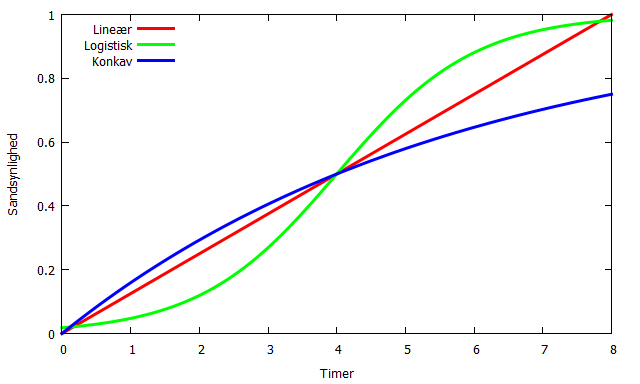
\includegraphics[scale=0.33]{graf-funktionseksempler}
	\caption{Tre funktioner til estimering af sandsynlighed for søvn}\label{fig:trefunc}
\end{figure}

\cref{fig:trefunc} viser tre forslag til en sådan funktion.
Disse er den røde lineære funktion, den blå konkave funktion og den grønne logistiske funktion \citep{wiki:LogisticFunction}.
Alle tre funktioner har til fælles at de er voksende, hvilket passer med vores antagelse af jo længere der har været stilstand jo større sandsynlighed er der for at man sover.
Den lineære funktion bygger på antagelsen, at sandsynligheden for at man sover er kongruent med stilstandslængden, hvilket vi ikke ønsker da vi så tillægger for stor vægt til korte stilstandsperioder. Imidlertid kan det godt være at den lineære og konkave funktion ville være bedre til at registrere korte søvnperioder midt om dagen.
Dette kræver videre arbejde men som en start benyttes den logistiske funktion, men kan nemt udskiftes.


Dn logistiske funktion beskriver hvordan at ved længere stilstandsperioder er der en forøget hældning i funktionen, indtil vi nærmer os lange stilstandsperioder hvor ekstra tid ikke giver en meget forøget sandsynlighed for søvn. 
Dette kan ses da den logistiske funktion vi har plottet går asymptotisk mod 1, svarende til 100\% sikkerhed for søvn.
I realiteten kan vi aldrig være 100\% sikker på søvn ved lang stilstand, da det kan være man har glemt sin smartphone hjemme mens man er på tur over en weekend, men hvis forudsætningen for at systemet fungerer er at man har sin smartphone i nærheden, regnes den logistiske funktion som et godt redskab til et søvnestimat.

Definitionen af den logistiske funktion er defineret som følger:
\begin{equation}
	f(t_{span}) = \frac{L}{1+e^{\,-k\cdot(t_{span} - t_{midtpunkt})}}
\end{equation} 
hvor,
\begin{itemize}
	\item[$L$] er kurvens maksimums værdi, hvilket for os eksempelvis kan være $1$ for 100\% sandsynlighed for at man sover.
	\item[$k$] er stejlheden for kurven.
	\item[$t_{span}$] Tidsperiode siden starten på stilstandsperioden målt i timer.
	\item[$t_{midtpunkt}$] Er det tidspunkt hvor kurven når $L/2$, hvilket i figurens tilfælde er hvornår kurven når $0.5$ det vil sige ved 4 timer.
\end{itemize}

Der kan argumenteres for en lavere værdi for $L$ så man maks kan blive 90\% sikker, men er noget der bør overvejes med mere træningsdata. 
Det kan også være en god idé at ændre på stejlheden for kurven, altså k, baseret på hvilken kilde af data man bruger som f.eks. accelerometer eller lyd.
Desuden skal $t_{midtpunkt}$ værdi på 4 timer betragtes som et første bud der passede fint med det observerede data, men kan justeres.

\subsection{Kombinering af modeller}\label{subsec:kombimodeller}
Det er tiltænkt at hver sensor kan have en tilknyttet søvnestimeringsmodel, hvilket i vores tilfælde er en søvnestimeringsmodel for accelerometret og en for amplituden.
Imidlertid kan det være en fordel at have en samlet model der kombinerer resultaterne fundet for de enkelte modeller.
En metode til dette er det vægtede gennemsnit og er et redskab vi har beskrevet i \cref{sec:redskaber}
Vores implementering af det vægtede gennemsnit afviger fra et normalt vægtet gennemsnit, idet at for de enkelte søvnestimeringsmoduler er der ikke blevet registreret data på samme tid eller i samme mængde.
På grund af dette tager modulet højde for hvis der er mangel på en estimering til en given tid for et af søvnestimeringsmodulerne.
Måden dette gøres er ved at tages den forrige værdi til estimeringen.
Man kan forestille sig en lynlås hvor der skiftes mellem takkerne fra hver del, på samme måde gøres med estimeringerne for hvert modul, for at illustrere dette bruges der et eksempel.

\newcommand{\nv}{Ingen estimering}

\begin{table}[h]
\centering
\resizebox{\columnwidth}{!}{\begin{tabular}{|c|c|c|p{2.5cm}|}
\hline Tid & Sandsynlighed for model A & Sandsynlighed for model B & Resultat\\ 
\thickhline 02:30:00 & 	0.59    & \nv  	& $\text{Vægt}_A * 0.59 + \text{Vægt}_B * 0.29$\\ 
\hline 02:30:01 & 	\nv     & 0.29 	& $\text{Vægt}_A * 0.61 + \text{Vægt}_B * 0.29$\\ 
\hline 02:30:02 & 	0.61    & \nv 	& $\text{Vægt}_A * 0.61 + \text{Vægt}_B * 0.30$\\
\hline 02:30:03 & 	0.62    & 0.30 	& $\text{Vægt}_A * 0.62 + \text{Vægt}_B * 0.30$\\ 
\hline 02:30:04 & 	0.63    & \nv 	& $\text{Vægt}_A * 0.63 + \text{Vægt}_B * 0.31$\\ 
\hline 02:30:05 & 	\nv     & 0.31 	& ...\\
\hline 
\end{tabular}} 
\caption{Tabel der illustrerer hvordan kombineringen fungerer. $\text{Vægt}_A$ og $\text{Vægt}_B$ er de fastsatte vægte for de to modeller.}
\label{tab:combiModelsExample}
\end{table}

I \cref{tab:combiModelsExample} kan man se kombineringen af de to modeller.
Måden den kombinerer sandsynligheder på er ved at den starter med to gennemløbere, henholdsvis for A og B, som starter på det første element som ikke er tom. 
Så derfor i eksemplet vil A starte ved 02:30:00 med værdien $0.59$ og for B vil den starte ved 02:30:01 med værdien $0.29$. 
Disse to værdier kombineres for det bagerste element med vægtningerne for de to modeller, hvorefter flyttes den bagerste gennemløber, og en ny kombinering foretages.
Dette forsætter indtil der ikke er mere data tilbage i en af de to gennemløbere, hvorefter der ventes på ny data så begge gennemløbere igen har data at køre på.

\subsection{Aggregering}\label{subsec:soevnaggre}
Som demonstreret giver søvnestimeringsmetoden, der er vist som proof of concept, en estimering til en lang række tidspunkter.
Men for at give et ekstra redskab til at danne et overblik over disse estimeringer, kan der med fordel som proof of concept laves en aggregering af søvnestimeringsdata.

For at få et bedre indblik i formen af data der skal aggregeres gives et eksempel i \cref{tab:noaggsoevndata}.
\begin{table}[h]
	\centering
\begin{tabular}{|c|c|c|}
	\hline {\_}id & prob & time \\ 
	\thickhline 203754 & 0.050 & 2015-04-26 01:41:42.446 \\ 
	\hline 203755 & 0.050 & 2015-04-25 01:41:43.375 \\ 
	\hline ... & ... & ... \\ 
	\hline 218777 & 0.919 & 2015-04-26 05:52:36.204 \\ 
	\hline 218778 & 0.919 & 2015-04-26 05:52:37.203 \\ 
	\hline 218779 & 0.000 & 2015-04-26 05:52:38.163 \\ 
	\hline 
\end{tabular}
\caption{Eksempel på søvnestimeringsdata, der ikke er aggregeret.}\label{tab:noaggsoevndata}
\end{table}
Ved at se på data som i \cref{tab:noaggsoevndata} fremstår det hvordan at fra {\_}id 203754 til {\_}id 218778 er sandsynligheden for søvn, der ses i \textit{prob} kolonnen, monotont voksende.
Idéen derudfra er så at registrere sådanne monotoniforhold og aggregere data med hensyn til det.
Det vil sige at registrere intervaller hvor \textit{prob} er tilpas stor over en længere tidsperiode, samt er monotont voksende.

Det blev besluttet at forkaste intervaller kortere end 10 minutter og hvor sandsynligheden for søvn i slutningen af intervallet er under 10\%.
Dette kan være en fornuftig løsning under antagelse af at man er rolig når man sover, og har da også vist gode resultater med nogle tests af personer med en meget rolig søvn. 
Eksempelvis med det viste data i \cref{tab:noaggsoevndata} vil dette blive aggregeret til en række som set i \cref{tab:aggdat}.

\begin{table}[h]
	\centering
\begin{tabular}{|c|c|c|c|}
	\hline {\_}id & startdate & enddate & prob \\ 
	\thickhline 1 & 2015-04-26 01:41:42.446 &  2015-04-26 05:52:37.203 & 0.919 \\ 
	\hline 
\end{tabular} 
\caption{Aggregering af data fra \cref{tab:noaggsoevndata}.}\label{tab:aggdat}
\end{table}

Vi har dog også fundet tilfælde hvor en aggregering ikke er akkurat, eksempelvis ved snorken fejler denne aggregering da den er for naiv, yderligere diskussion om hvad man kan gøre i stedet for er beskrevet tidligere i \cref{section:snorken}.
Et alternativ kunne være at tage arealet af søvnestimeringsdata, og bruge arealet som estimat til hvor meget man har sovet per dag.
Dette har ulempen at det ikke vil oplyse om selve søvnperioderne men blot mængde af søvn per dag, derudover vil den stadig blive påvirket af snorken og andre støjfaktorer.
Vi hæfter os ved at denne aggregeringsmetode er ment som et proof of concept og med ekstra ressourcer kan det være fornuftigt at se på andre aggregeringsmetoder og inddrage fundne snorken estimeringer til at kunne aggregere søvndata på mere akkurat vis. Forslag til dette kan læses i \cref{section:snorken}.

\subsection{Visualisering}\label{sec:pocVis}
For at kunne vise brugeren af systemet hvordan deres søvn har været, skal der tilføjes nogle visningsmoduler.
Disse visningsmoduler skal kunne give et overblik over hvordan man har sovet den seneste nat, men også hvordan man har sovet det seneste stykke tid.

For at kunne udtrykke dette til brugeren er der først blevet lavet en graf der viser hvor sikker systemet er på at man har sovet over en periode.
Denne periode er sat til at være alt data der er på smartphonen så brugeren har overblik over ændringer i grafen.
Disse ændringer kan derved indikere at der er sket en ændring i ens sindstilstand.
Til at sørge for at grafen kan bruges til både at se hvordan man har sovet over en længere periode samt over en kort periode, har man den mulighed at man kan zoome på grafen, og derved se præcis hvor sikker systemet er på man har sovet på et bestemt tidspunkt.
Der er også lavet en graf for hvor sikker systemet ved hjælp af kun acceleration er på at man sover, det samme gælder for lyd, se \cref{fig:visningsgrafer}.

\begin{figure}[h]
	\centering
	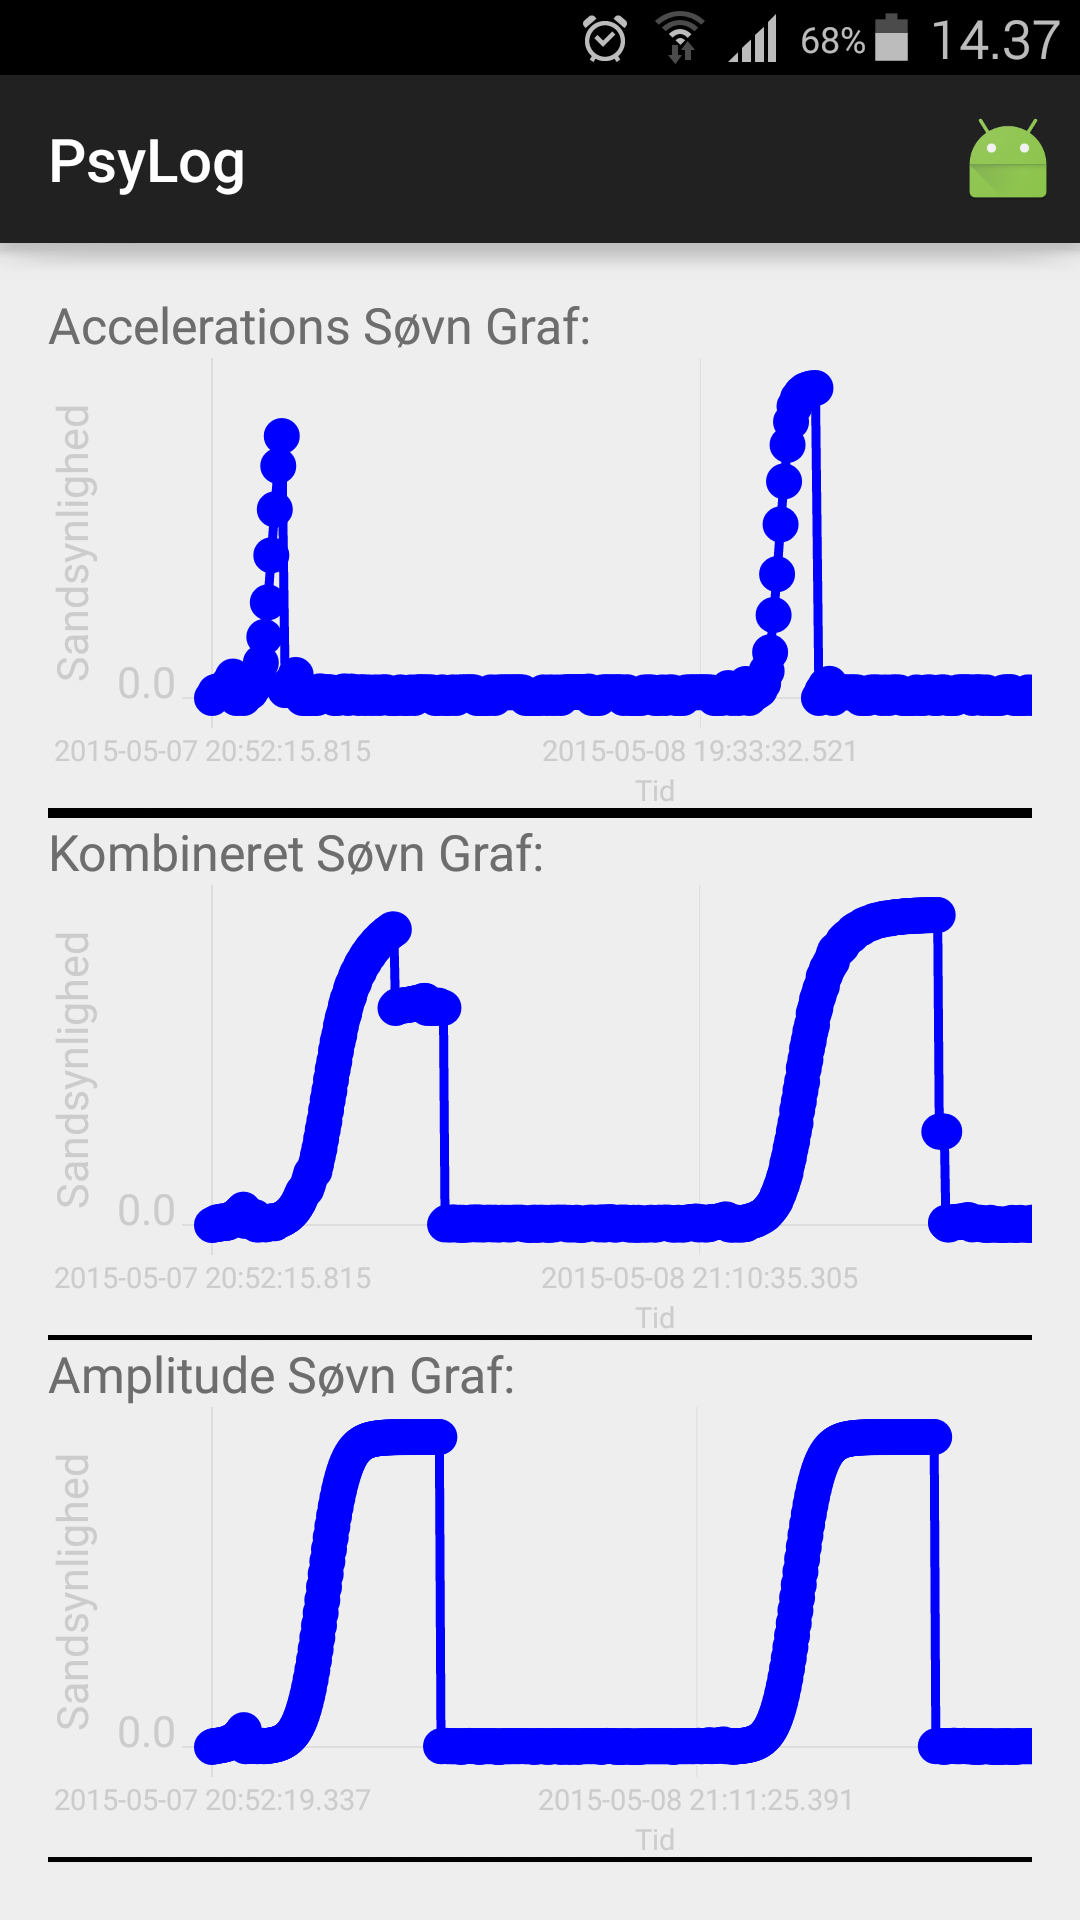
\includegraphics[scale=0.1]{visningsgrafer}
	\caption{Tre funktioner til estimering af sandsynlighed for søvn}\label{fig:visningsgrafer}
\end{figure}

Grafer er dog ikke altid lige nemme at forstå, derfor er der blevet lavet en tabel der viser hvor sikker systemet er på at man har sovet over en periode.
Denne tabel minder om den der blev vist i \cref{tab:aggdat}, dog uden $\_id$ kolonnen.
Tabellen giver et nemt overblik for brugeren om hvornår man har sovet, samt hvor sikker systemet er på at man har sovet.
Dog er det ikke så nemt for brugeren at se ens adfærdsændring i en sådan tabel, da det kræver at man kigger på meget data på en gang.
Som alternativ kan der ses på et 'early warning modul', og er diskuteret i \cref{chap:bigdisc}.
% Giv eksempel på ikke aggregeret data.
% Forklar forslag/løsning til aggregering af data.
% Vis resultat derfor
% Diskuter problemer? (e.g. snorken) evt. referer til snorken diskussion
\subsection{Eksempel}
Gennemgangen af metoden er beskrevet for i detalje for hver del, men det kan være svært at få overblikket over metoden.
Af denne grund gives her et eksempel der tager en fra de rå data og hele vejen til det aggregerede resultat.
Eksemplet der følges kan ses i \cref{fig:totalbanjo}.
%intro godt at give et eksempel
%gennemgang af hvert led
%resultatet er at man har regnet ud der soves derfra og dertil
\begin{sidewaysfigure}
	\begin{minipage}{0.2\textwidth}
		\begin{subfigure}{\linewidth}
			\centering
			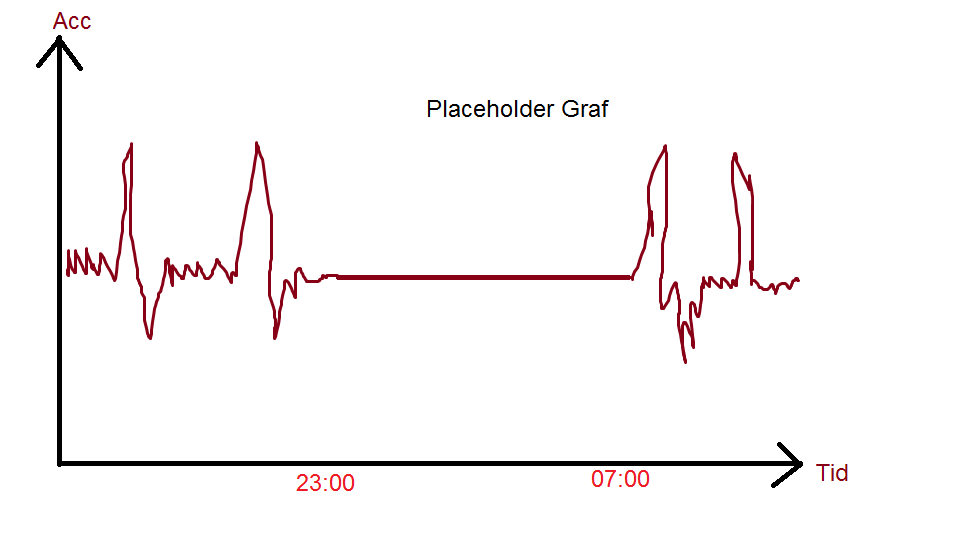
\includegraphics[scale=0.2]{acc-placeholder}
			\caption{Rå accelerations data.}\label{fig:rawaccplot}
		\end{subfigure}\\[5ex]
		\begin{subfigure}{\linewidth}
			\centering
			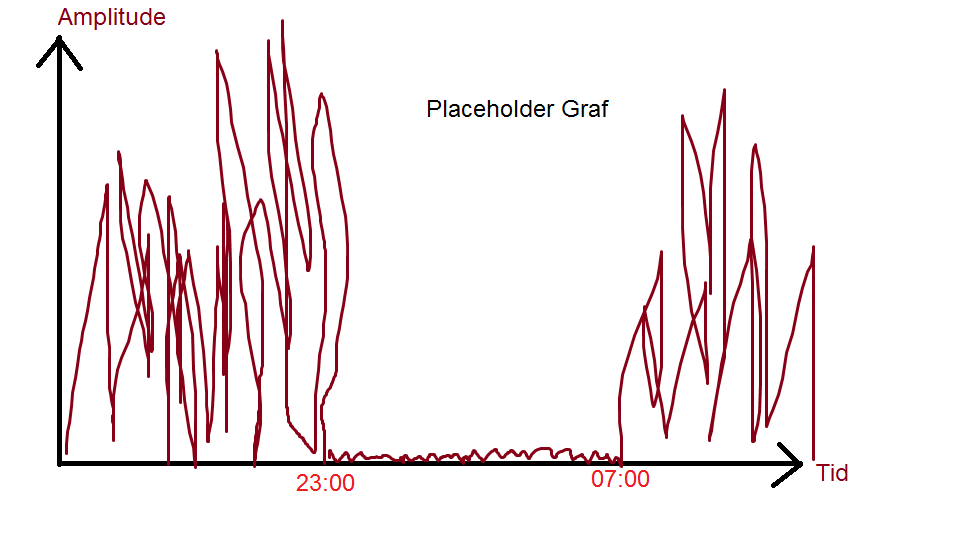
\includegraphics[scale=0.2]{ampl-placeholder}
			\caption{Rå amplitude data.}\label{fig:rawamplplot}
		\end{subfigure}
	\end{minipage}%
	\begin{minipage}{0.1\textwidth}
		\begin{subfigure}{\linewidth}
			\centering
			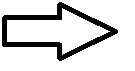
\includegraphics[scale=0.3]{arrow}
		\end{subfigure}\\[15ex]
		\begin{subfigure}{\linewidth}
			\centering
			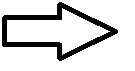
\includegraphics[scale=0.3]{arrow}
		\end{subfigure}
	\end{minipage}%
	\begin{minipage}{0.2\textwidth}
		\begin{subfigure}{\linewidth}
			\centering
			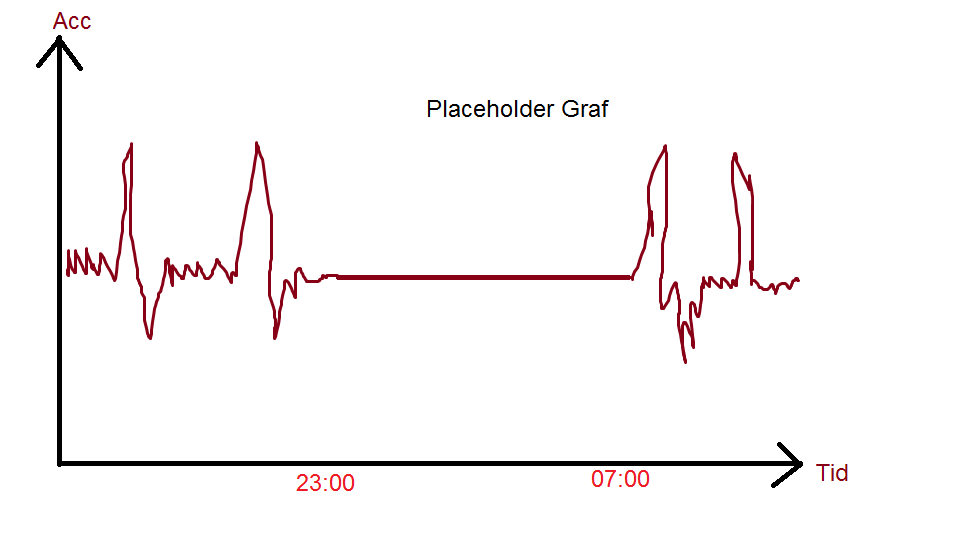
\includegraphics[scale=0.2]{acc-placeholder}
			\caption{Accelerations søvnestimering.}\label{fig:sleepcalcaccplot}
		\end{subfigure}\\[5ex]
		\begin{subfigure}{\linewidth}
			\centering
			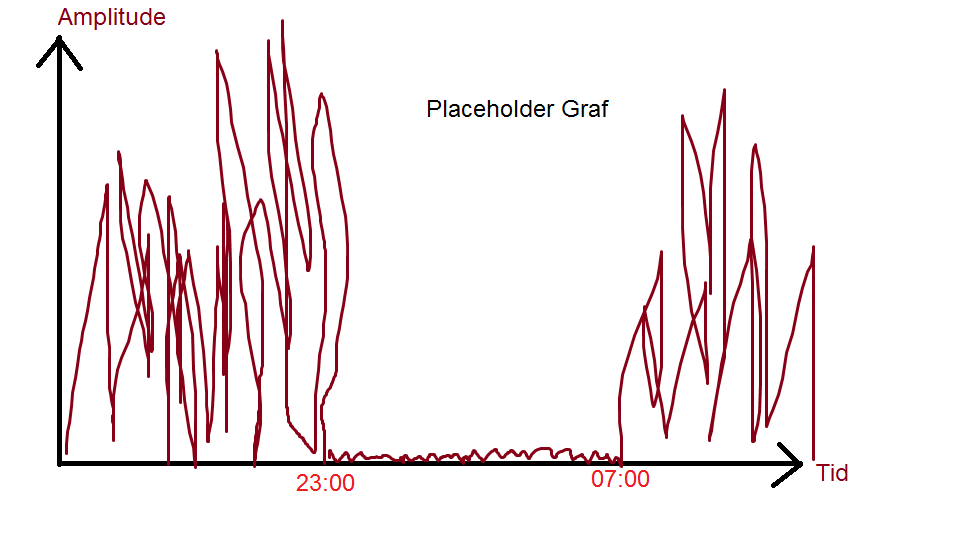
\includegraphics[scale=0.2]{ampl-placeholder}
			\caption{Amplitude søvnestimering}\label{fig:sleepcalcamplplot}
		\end{subfigure}
	\end{minipage}%
	\begin{minipage}{0.1\textwidth}
		\begin{subfigure}{\linewidth}
			\centering
			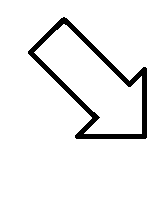
\includegraphics[scale=0.2]{downarrow}
		\end{subfigure}\\[15ex]
		\begin{subfigure}{\linewidth}
			\centering
			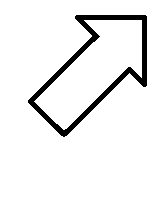
\includegraphics[scale=0.2]{uparrow}
		\end{subfigure}
	\end{minipage}%
	\begin{minipage}{0.2\textwidth}
		\begin{subfigure}{\linewidth}
			\centering
			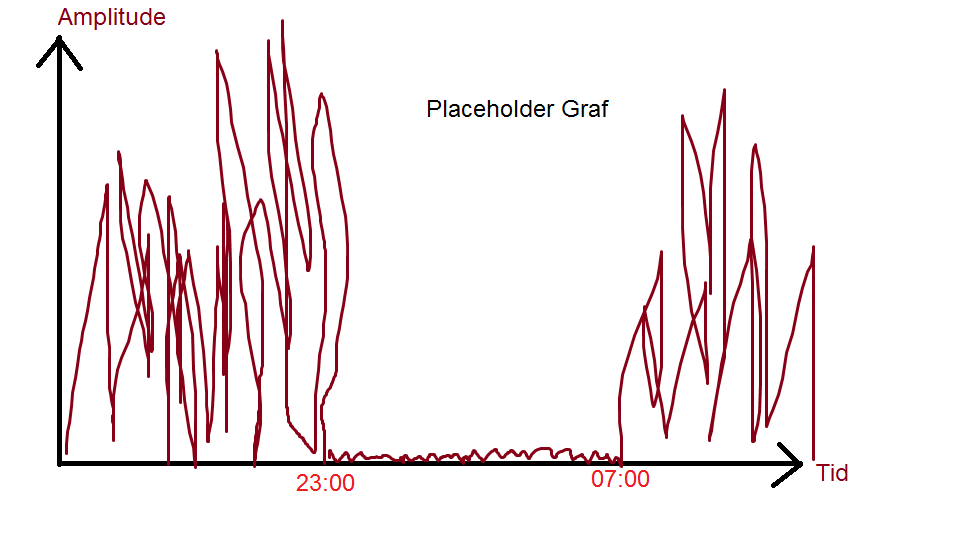
\includegraphics[scale=0.2]{ampl-placeholder}
			\caption{Kombineret søvnestimering}\label{fig:sleepcalcombine}
		\end{subfigure}
	\end{minipage}%
	\begin{minipage}{0.1\textwidth}
		\begin{subfigure}{\linewidth}
			\centering
			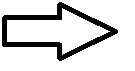
\includegraphics[scale=0.3]{arrow}
		\end{subfigure}
	\end{minipage}%
	\begin{minipage}{0.07\textwidth}
		\begin{subfigure}{\linewidth}
			\centering
			\rotatebox{270}{\begin{tabular}{|c|c|c|}
			\hline starttid & sluttid & sandsynlighed \\ 
			\hline 20-20-2015 00:01 & 20-20-2015 08:05 & 0.99 \\ 
			\hline 
			\end{tabular}}
			\caption{Aggregering.}\label{fig:finalagg}
		\end{subfigure}
	\end{minipage}
	\caption{Illustration af søvnestimering fra rå data til aggregering.}\label{fig:totalbanjo}
\end{sidewaysfigure}

Der startes med de rå accelerations og amplitude data der kan ses i \cref{fig:rawaccplot} og \cref{fig:rawamplplot}.
På dette dataset foretages en række metoder beskrevet blablabla.
\subsection{Verificering}
Med søvnestimeringsmetoden udviklet som proof of concept, er det nødvendigt at få verificeret at den har en tilfredsstillende præcision, hvilket er et af de primære kriterier nævnt i \cref{sec:metodevalg}.
For at tjekke dette kan vi inddrage en mere sikker søvnestimeringsmetode såsom polysomnografi, hvilket ville være et oplagt valg, da det er state of the art indenfor søvnestimering og er beskrevet i \cref{sec:polysomnografi}.

Vi er dog ikke begrænset til polysomnografi, det vigtigste er at det er en metode, der er så præcis som mulig, da den skal bruges til at verificere resultatet.
Dette skal ses i en testsammenhæng, så kriterier om at den skal være non-intrusive gælder ikke her.

Fremgangsmåden til at teste om den udviklede estimeringsmetode er tilstrækkelig går så på at have en af række personer, der sove hvor man både estimerer med brug af vores model og med brug af den valgte absolutte sandheds metode.
På den måde vil man kunne indsamle resultater fra begge metoder og derved sammenligne ens estimat med den absolutte sandhed.

I tilfælde af en ikke tilstrækkelig præcision kan der forsøges at justere på de forskellige værdier i systemet for at se hvilken effekt det har på præcisionen.
Kandidater til disse ændringer kan være:
\begin{itemize}
	\item Konstanter for antal målinger, der skal overvejes for at bestemme stilstand eller stilhed, og muligvis se på tidsintervaller i stedet for målinger.
	\item Grænseværdier for hvor sandsynligheden skal være før en periode vurderes til at være en søvnperiode.
	\item Middelværdien for den logistiske funktion, idet at dette vil ændre hvor lang tid det vil tage før sandsynligheden vil nå 50\%.
\end{itemize} 

Hvis dette gøres vil man få et indtryk af hvordan de konstanter påvirker vurderingen, og så er man forhåbentlig i stand til at komme med en konfiguration af disse, der har en tilpas høj nøjagtighed.
Vi hæfter os ved, at når man justerer på diverse parametre for modellen, bør præcisionsestimatet vurderes ved hjælp af krydsvalidering.
Som nævnt i \cref{sec:redskaber}, er krydsvalidering en metode der bruges til at vurdere en model og hvordan den model vil fungere når den bruges på andre datasæt, idet at en model kan blive for tilpasset til ét præcist datasæt hvori problemet ligger i at modellen ikke vil fungere ved andre datasæt.

I tilfælde af en ikke tilfredsstillende præcision, selvom man har justeret på disse parametre, bør man overveje at erstatte metoden med en anden.
Sådanne metoder er undersøgt i \cref{sec:metodevalg} og man kan med fordel starte med de deri nævnte.
Vi har tilstræbt at fremtidssikre vores produkt, sådan at dette ikke skulle volde problemer grundet den modulære platform.\label{sec:verisoevn}
\section{Videre arbejde}\label{sec:videre-arbejde}
Denne sektion detaljerer problemer som er tiltænkt skal løses ved videre arbejde på systemet da den implementerede proof of concept har problemer med dem. 
Dette inkluderer at folk snorker når de sover og vores proof of concept tager ikke højde for dette, kombinering af sensor data er ikke optimal og kunne gøres bedre, afbrudt og dårlig søvn kan ikke registreres af systemet men bare søvnlængde og til sidst at der er mange sensorer som ikke bliver brugt som måske kunne bringes ind.
\subsection{Sensor Vægtning}\label{subsec:sensorvaegtsoevn}
Som nævnt er vægtningen mellem vores sensorer sat til statiske værdier.
Dette blev valgt fordi det var en simplere løsning for både udviklere og brugere, da disse faste værdier gør at en læringsperiode ikke er nødvendig, og at systemet derfor kan bruges direkte.

At vægtningen er statisk kan være problematisk, da alle individer anses som værende forskellige. 
Eksempelvis er nogle personer mere støjende end andre.
En støjende person skal forstås som en der taler, banker i bordet, eller på anden vis forårsager en høj registreret amplitude.
En stille person er en der ikke forårsager disse høje amplituder.
Ved en stille person kunne det være man skal give søvnestimeringen baseret på lyd en mindre vægt, efnd for en støjende person der er stille når han sover.
Dette skyldes at en stille person der snorken om natten, ud fra amplitude-data ville blive vurderet til at sove om dagen og være vågen om natten, selvom dette ikke er tilfældet.

Hvis vi vil have vores sensor vægtning, og dermed vores søvnestimering, til at være mere tilpasset individet, vil det være nødvendigt at tilføje en læringsperiode med data, der kan anses for den absolutte sandhed.
Dette træningsdata kan eksempelvis indsamles ved at lade patienten holde en dagbog for deres søvn, samtidig med at man indsamler sensor data.
Denne indsamling vil så køre i en periode, og modellen vil så kunne tilpasses den enkelte patient.

Baseret på dette vil det så være muligt at lave en model til at finde den bedste vægtning af datakilder.
Den bedste vægtning værende den hvor nøjagtigheden af vurderingerne er så høj som muligt.

Implementeringen vil også kræve længere testperioder end dem vi har brugt.
De nuværende testperioder vi har brugt, har været på en til to dage, hvorimod med en læringsmodel vil en længere og sandsynligvis todelt testperiode være nødvendig, der er benyttet i \citet{6563918} og \citet{Min:2014:TNT:2556288.2557220}.
I de to artikler har de brugt en læringsperiode på henholdsvis en uge og tre dage så et sted imellem disse to vil nok være en fornuftigt minimumsgrænse
Perioden skal være længere end dem vi har brugt, da der er brug for mere data til at lave en ordentlig læringsmodel med procent vægtning, og den bør være todelt så man har noget data man kan teste sin endelige model på, som ikke har været brugt til at lave modellen.

\subsection{Søvnkvalitet}
Ved fokusgruppeinterviewet, se \citep[Kapitel 1, Sektion 5]{misc:faellesrapp}, blev der fortalt at et af problemerne som patienterne ved interviewet personligt oplevede var, at de generelt sover dårligt under en depression.
Endvidere, har en psykiater samt en psykolog fortalt os at personer med affektive lidelser ofte oplever en søvnforandring, se \citep[Kapitel 1, Sektion 3 og 4]{misc:faellesrapp}.
Eksempel på dette kan være at deres søvn er meget afbrudt, at de har det svært ved at falde i søvn og at de ikke sover særlig længe.

Det der for det meste er blevet fokuseret på er at måle søvnlængde, ses der dermed ikke på aktuelle søvnkvalitets indikatorer som f.eks. urolighed, hvor lang tid det tager dem at falde i søvn og hvor afbrudt søvnen er.
Søvnlængde er en god indikator og hvis man kan finde en måde at måle dette, kan man med fordel få en god idé om hvordan det går med patienten ved blot at se på forandringer i søvnmønstret. 
Hvis man dog vil have det fulde billede af søvn, skal man også se på søvnkvalitet, da hvis en person vågner hele tiden, men ikke larmer eller rører sin telefon, bliver dette registreret som en lang søvn periode.
\subsection{Ubrugte Sensorer}
Vores proof of concept til søvn estimering var 'Best Effort Sleep', se \cref{sec:BES}, som inkluderer 6 forskellige datakilder og vi bruger kun 2 af dem: Lyd og bevægelse. 
Dette blev gjort idet at de andre sensorer ikke var givet en særlig stor vægtning i forhold til lyd og bevægelse, da de alle havde vægtninger under 6\%. 
Dette betyder selvfølgelig ikke at de er værdiløse bare at de ikke er så vigtige som de to primære kilder.
Men det vil stadigvæk være en god idé at undersøge disse ubrugte data kilder og se om de har nogen stor effekt på den endelige sandsynlighed idet at hvis metoden kan gøres mere akkurat ville det selvfølgelig være godt. 
Det er dog bare de data kilder som der er kendt fra \cref{sec:BES}, og der er sandsynligvis andre kilder som kan inkluderes og undersøges.
Dette kunne f.eks. være placering hvor man kan se om personen er hjemme og hvis personen ikke er, så kan man antage at der vil være en mindre sandsynlighed for at de sover. 
\subsection{Visualisering}\label{sec:soevnVisVidArb}
Visualisering af analyse resultater er kun blevet udforsket i begrænset omfang, selvom den visuelle repræsentation er yderst essentiel i afgørelsen om systemet kan bruges, da denne er forbundet til kriteriet om at brugerne selv skal kunne bruge det uden hjælp, beskrevet i \cref{sec:metodevalg}.
Hvis visningsmoduler skal implementeres på et tilfredsstillende niveau, kræver det at der bliver udforsket datavisualiserings-teknikker og -teorier.
Det vigtigste her ville så være at finde en visualiserings-form, der giver den information brugeren leder efter eller har brug for, på en sådan måde at brugere selv kan forstå hvad der vises på skærmen.
En anden ting der er vigtig når visningsmoduler skal laves er, at det ikke er nok med en, da folk med forskellig baggrund forstår ting forskelligt, derved kan det være at den visualisering der kan være indlysende for en person, kan være fuldstændig uforståelig for en anden.
Det problem er en af hovedårsagerne til, at visualisering har fået så lidt opmærksomhed som det har, det er simpelthen et projekt i sig selv at lave noget, der er forståeligt for så bred en gruppe folk som dette system er tiltænkt til.
Ydermere kan denne målgruppe også være vanskelig at få adgang til, da de er yderst sårbare rent mentalt, dette kan dog arbejdes udenom ved at bruge ikke-affektivt lidende personer til de første tests.
Dog er der lavet et proof of concept af visningsmoduler, der er beskrevet i \cref{sec:pocVis}.



\chapter{Fysisk Aktivitet}
Dette kapitel beskriver fysisk aktivitets delen af projektet.
Fysisk aktivitet er tiltænkt som en ekstra komponent udover søvn, der kan integreres i platformen.
Tankegangen med at benytte fysisk aktivitet er at det komplementerer søvn, da det muliggør en dækning af hele dagen og ikke blot natten.
Der er også en mulighed for, at fysisk aktivitet kunne give et signal om søvnkvalitet ud fra gangmønster.
Idéen er at hvis man har sovet dårligt og er træt, påvirker dette ens gang.
Dette er blot en teori, men kan med fordel undersøges med videre arbejde.

Før vi kan tale om fysisk aktivitet er der nødt til at blive opstillet en fælles forståelse af hvad fysisk aktivitet og inaktivitet indebærer.
\begin{description}
\item[Fysisk aktivitet] er en tilstand af kropslig bevægelse, hvor vi ser fysisk aktivitet som gang eller mere \citep{misc:PhysicalActivity}.
\item[Fysisk inaktivitet] er en tilstand hvor kropslig bevægelse er nedsat, modsat fysisk aktivitet.
\end{description}
\section{Forskning}
Denne sektion beskriver forskningen, der undersøger forbindelsen mellem psykiske lidelser og fysisk aktivitet. 
Dette er vigtigt for at danne et overblik over hvad der overhovedet kan gøres med fysisk aktivitet, og til hvilke slags personer løsningen skal tilrettes.
Endvidere diskuteres der hvilke sensorer, der kan bruges til at måle fysisk aktivitet, såsom accelerometer, stepcounter og GPS.
Ydermere, diskuteres det proof of concept der implementeres for fysisk aktivitet og hvordan denne aggregeres. 

I vores samtaler med eksperter indenfor psykiatri feltet \citep[Kapitel 1, Sektion 3 og 4]{misc:faellesrapp}, blev det klart at de mente fysisk aktivitet var vigtigt i behandling af psykiske lidelser.
Det samme er sandt for fokusgruppeinterviewet, hvor vi igen blev fortalt at fysisk aktivitet hjælper \citep[Kapitel 1, Sektion 5]{misc:faellesrapp}.
Dette understøttes også af mange kilder, der har undersøgt en sammenhæng mellem fysisk aktivitet og symptomerne for depression. \citet{art:physDepSymptoms, Strawbridge15082002, Arredondo01072012} er blandt andet nået frem til at en sådan sammenhæng bestemt virker til at være reel.
Selvom kilderne ikke direkte siger at nedsat fysisk aktivitet er et symptom på begyndende depression, så er den sammenhæng de når frem til mellem depressions symptomerne og fysisk aktivitet nok til, at vi godt kan vurdere nedsat fysisk aktivitet som et symptom, da det gør tilstedeværelsen af andre symptomer mere alvorlige.

Derudover, har vi fundet kilder der også indikerer at det kan gå den anden vej, hvor forøget fysisk aktivitet er et tegn på bedring for depressive patienter.
Først har vi \citet{misc:healthReports} fra 1985, der siger at det ser ud til at være en sammenhæng, ikke blot mellem fysisk aktivitet og depression, men også med angst, mentalt handikap og andre former for psykiske lidelser.
Her var det muligt at finde nyere materiale, der understøtter forbindelsen mellem fysisk aktivitet og depression samt angst, hvilket er beskrevet herefter.

I \citet{art:physMental} fra 2000 er der blevet set på en større mængde undersøgelser, og de er nået frem til en række implikationer, der kan være for klinisk behandling.
Blandt disse implikationer er, at individer diagnosticeret med svær depression eller individer der har brug for psykologisk behandling, viser de største forbedringer ved øget fysisk aktivitet.
Derudover, er der også en implikation, der viser at fysisk aktivitet virker lige så effektivt som psykologisk terapi til at mindske effekten af depressions symptomer hos folk med mild eller moderat depression.

Ifølge \citet{book:sportPsyc} er der fundet en forbindelse mellem fysisk aktivitet og forbedring i tilstanden hos mange patientgrupper, heriblandt personer med angst, depression og stress.
Ydermere, præsenterer de også et eksperiment, hvor en række angst patienter testede effektiviteten af medicinsk behandling overfor en fysisk træningsplan og en kombination af disse.
Eksperimentet viste at selvom den medicinske behandling virkede bedre i starten, gav alle tre ca. samme resultat.
Efterfølgende viste det sig også, at de folk der havde været en del af det fysiske aktiveringsprogram, havde en væsentlig mindre risiko for tilbagefald.

Alle tre kilder sætter fokus på fysisk aktivitet som behandlingsmetode, \citet{art:physMental} og \citet{book:sportPsyc} har resultater der understøtter denne holdning, hvorimod \citet{misc:healthReports} kun har formodninger om at det virker.

Grundet disse resultater, virker det logisk at give folk mulighed for selv at overvåge deres egen fysiske aktivitet, hvilket for eksempel kunne gøres via deres smartphone, da der er mange sensorer i en telefon der kan give information om dette.
Denne egen ansvarlige overvågning af fysisk aktivitet kan lægge dele af ansvaret for behandling og forhindring af tilbagefald over på patienten selv, og kan forhåbentlig forhindre en del indlæggelser.
Grunden til dette, er at hvis en patient bliver gjort opmærksom på at deres aktivitetsniveau falder, har de mulighed for at reagere før det er for sent.

\subsection{Sensorer til Fysisk Aktivitet}
I en smartphone er der mange sensorer, som kan bruges til at få et indblik i den fysiske aktivitet hos telefonens ejer.
Den primære sensor her er en stepcounter, der findes standard i alle android telefoner med API version 19 eller derover, men som også kan laves manuelt ved hjælp af accelerometret.
Udover stepcounteren, som giver et fint indblik i hvor mange skridt man tager, kan man også bruge GPS til at se på hvor langt man går.
Derudover, kan man også, for at være sikker på man logger den rigtige person, bruge telefonens accelerometer data til at beregne gangarten \citep{4272626} og ud fra den vurdere om det er telefonens ejer der har telefonen, eller om det er en anden person der har lånt telefonen.
Hvis det er en anden person der har telefonen, bør denne aktivitet fjernes fra data der bruges for beregninger til fysisk aktivitet hos patienten.

Hvis man føler der er for stor risiko for at telefonen ikke får det hele med, da det eksempelvis kan være irriterende at have sin telefon med ude at løbe, kan man gøre brug af andre former for måleudstyr.
Eksempelvis kan man her bruge smart earplugs eller et smart wristband, der begge har en række indsamlingsmetoder, som kan bruges til at indsamle data af samme type som fra en smartphone.
%\section{Metode Valg}
\section{Proof of Concept}
Baseret på den viden der er blevet indsamlet, laves der er et proof of concept til søvndelen af projektet.
Denne implementering er beskrevet herunder.
Grunden til at der kun laves et proof of concept og ikke et fuldstændigt færdigt system er, at der ikke er nok tid til at gøre det helt færdigt. 
Ydermere, vil et helt færdigt system påkræve testning hos målgruppen, og dette er der ikke er tid nok til at udføre. 

Denne sektion om proof of concept beskriver valg af nødvendig sensor data, hvordan søvnestimering udføres på data, og hvordan søvnestimeringerne for de forskellige sensorer kombineres og hvordan denne estimeringen skal aggregeres til individuelle perioder af søvn.

% Manglende resourcer
% Time constraints.
% Ingen test mulig(Kræver tilladelser, og system ikke færdig)

Som et proof of concept er der blevet valgt at implementere en enkelt metode til at afgøre hvorvidt man sover eller ej.
Metoden er baseret på redskaberne beskrevet i \cref{sec:redskaber}, hvor der som start til dataindsamling ses på amplitude og acceleration.
Grunden til at vi starter med disse to datakilder er fordi \citet{6563918} erfarede, at det er de langt væsentligste datakilder, hvilket også er beskrevet i \cref{sec:BES}.

Disse to datakilder kombineres til en enkelt model, der skal kunne afgøre hvorvidt man sover eller ej.
Med mere tid vil de andre nævnte datakilder også blive fokuseret på.

For at have en regelmæssig måde at indsamle data, der ligger til grund for implementeringen af det efterfølgende søvnestimeringsmetode, er det nødvendigt at have forsøgsopstillingen beskrevet, hvorfor denne følger herefter.
\subsection{Forsøgsopstilling}
%Disposition:
%Billede af opstilling
%Bare tage med hjem og sove
%Flere forsøg og systematisk tilgang kunne være brugt og skulle gøres hvis det ikke bare var proof of concept.
For at forsøget fortages på samme måde hver gang, så det indsamlede data er sammenligneligt, valgte vi at lave en forsøgsopstilling.
\begin{figure}[h]
	\centering
	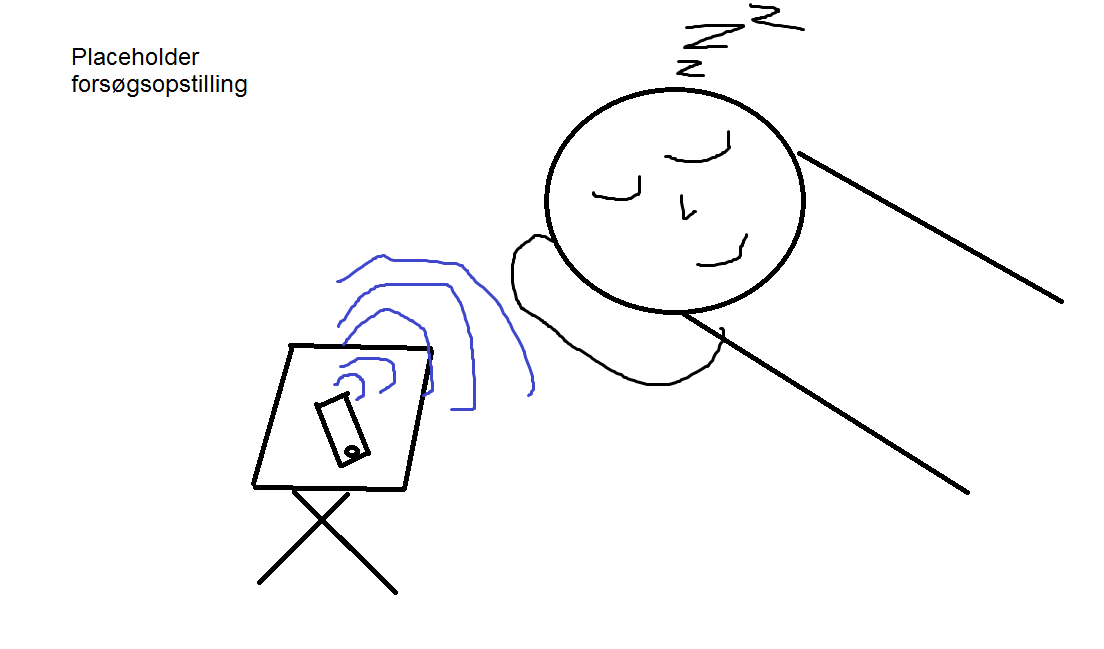
\includegraphics[scale=0.5,trim = 0cm 0cm 5cm 10cm, clip]{forsoegsopstilling}
	\caption{Forsøgsopstilling. Sovende person med smartphonen på natbordet.}
	\label{fig:forsoegopstillings}
\end{figure}

Forsøgsopstillingen kan ses i \cref{fig:forsoegopstillings} der illustrerer hvordan smartphonen ligger på natbordet og indsamler data.
Idéen er at det eneste krav til indsamlingen er, at den skal ligge på et bord i soveværelset når der soves, ellers står det en frit om man går med smartphonen i lommen, lægger den på skrivebordet eller andet. 
Dette valg er foretaget i henhold til vores kriterie om at udvikle et system der kan måle søvn uden at forstyrre.

Indsamlingen af data foregik ved at vi installerede de fornødne moduler på egen smartphone, Tog smartphonen med hjem, så data fra en eller flere dage kunne indsamles.
Vi loggede fra vi gik i seng til vi stod op, hvilket skulle bruges til at afgøre nøjagtigheden af vores estimat.

Til at validere vores model har vi foreslået krydsvalidering beskrevet i \cref{sec:redskaber}, hvilket også bør gøres med mere tid, men da dette er et proof of concept er den nuværende opstilling tilfredsstillende.
Ved videre arbejde bør en mere systematisk tilgang med den nævnte krydsvalidering benyttes, hvilket er beskrevet videre i \cref{sec:verisoevn}.

\subsection{Sensor Data}
For at have en bedre indsigt i hvordan vi kan bruge accelerations- og amplitude-data blev disse plottet over en dag inklusiv søvn.
Dette kan ses i \cref{fig:accplot} og \cref{fig:amplplot}.

\begin{figure}[h]
	\centering
	%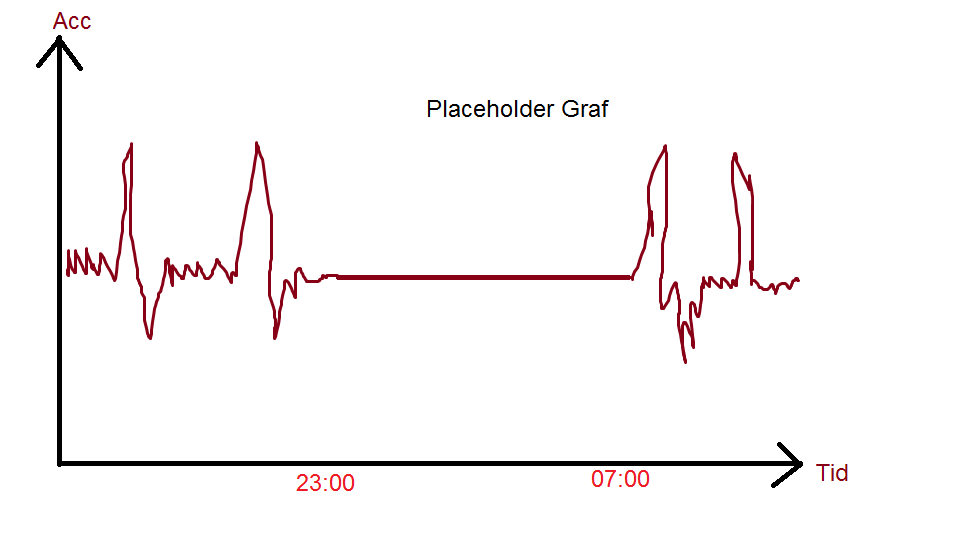
\includegraphics[scale=0.5]{acc-placeholder}
	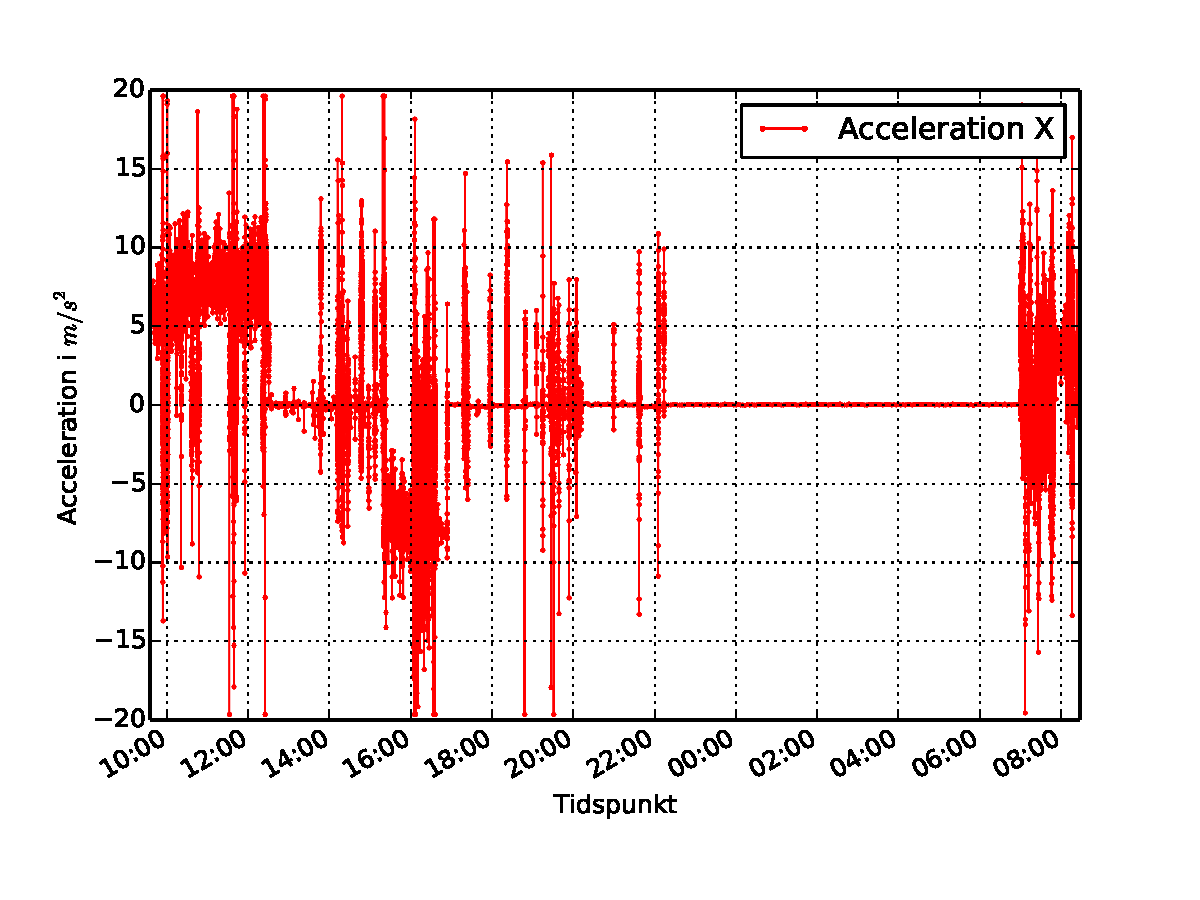
\includegraphics[scale=0.75]{acceleration-plot}
	\caption{Accelerationsplot, hvor der blev sovet fra ca. 22:00 til 07:00 næste dag.  Et punkt svarer til en måleværdi.}\label{fig:accplot}
\end{figure}

Ses der på accelerationsdata i \cref{fig:accplot} indikerer det tydeligt når smartphonen har været i bevægelse og når smartphonen ikke har været i bevægelse.
Dette skyldes at et accelerometer er god til at registrere bevægelse, da acceleration er ændring i hastighed.
Det viser sig at plottet fint indikerer når man er vågen, hvilket er forårsaget af at testpersonen har gået med sin smartphone i lommen.
Dog kan man ved stilstand ikke vide sig sikker på om det er fordi man sover, eller blot fordi man har lagt sin smartphone fra sig.

Ved stilstand i en længere periode, kan man estimere sandsynligheden for at denne stilstand er at brugeren sover. 
Derudover kan andre sensor inputs hjælpe til at klargøre denne tvivl, der ikke er begrænset til at man skal have smartphonen i lommen.
Et eksempel på en sådan kilde er mikrofonen, som vi kan bruge til at måle maks amplitude.
At vi kun måler maks amplitude sikrer at personfølsomme oplysninger ikke indsamles, da man ikke kan genskabe en samtale, men blot har maks amplitude lagret for hvert sekund.

\begin{figure}[h]
	\centering
	%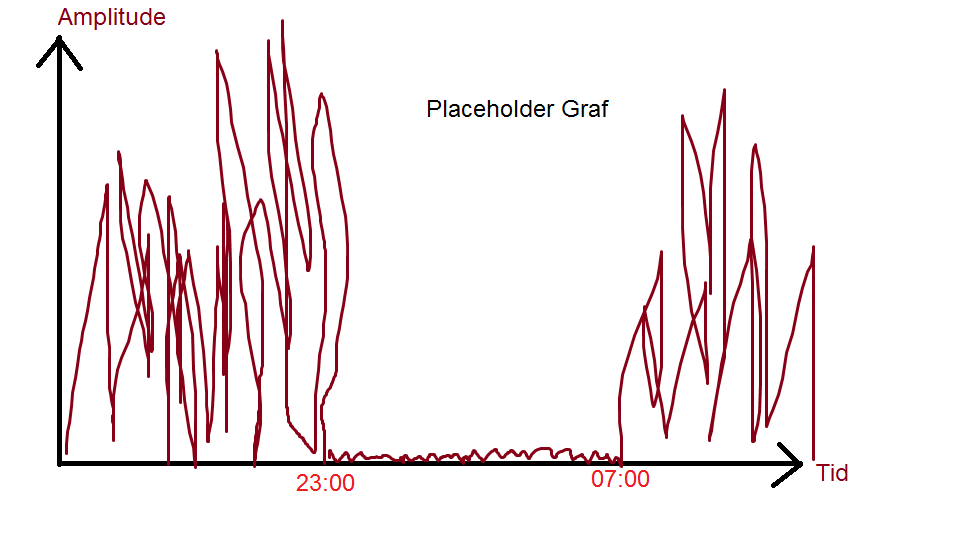
\includegraphics[scale=0.5]{ampl-placeholder}
	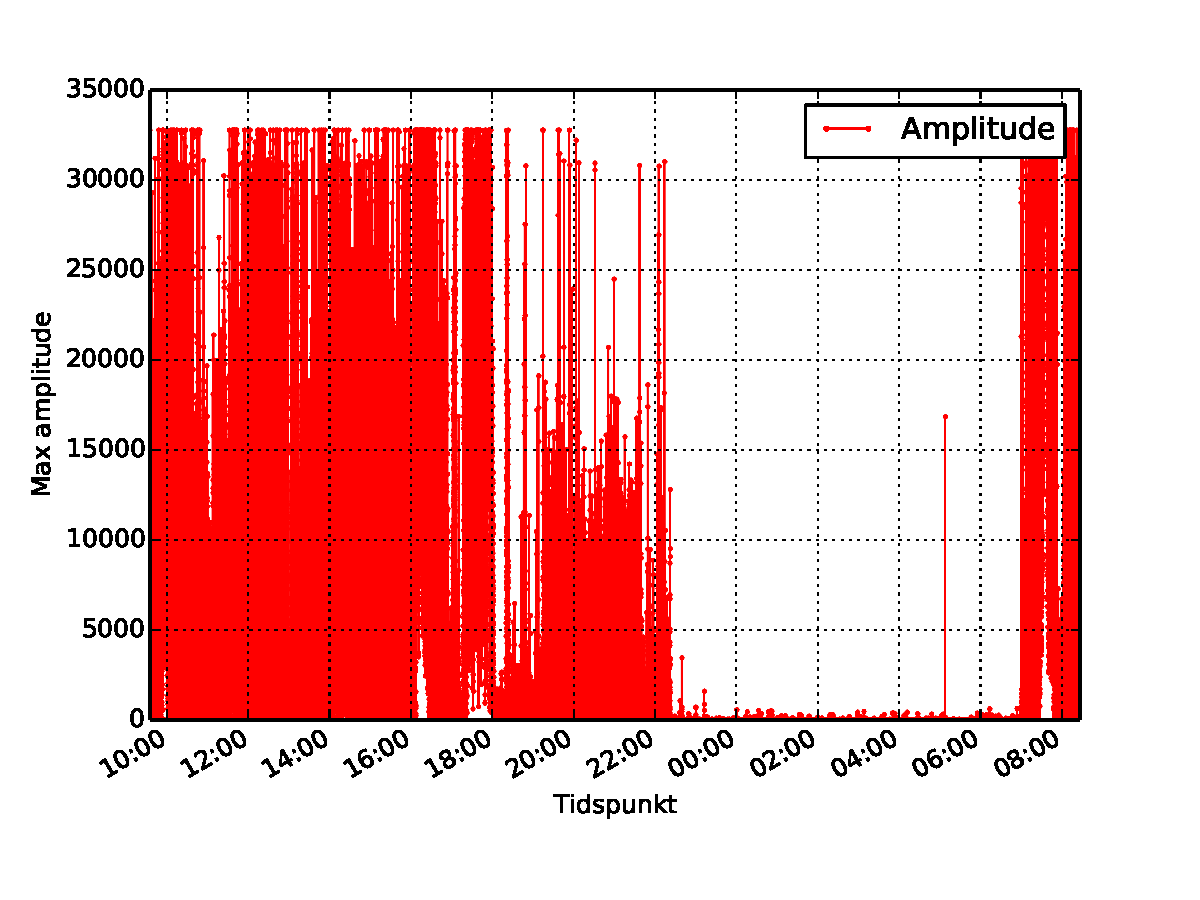
\includegraphics[scale=0.75]{amplitude-plot}
	\caption{Amplitudeplot, hvor der blev sovet fra ca. 22:00 til 07:00 næste dag. Et punkt svarer til en måleværdi.}\label{fig:amplplot}
\end{figure}

Idéen bag at bruge maks amplituden er at man larmer væsentligt mere når man er vågen end når man sover.
Dette passer fint med de loggede data der er plottet i \cref{fig:amplplot}.
Dog har denne antagelse også begrænsninger.
Eksempelvis kan det være at man er en stille person, snorker meget eller også kan personen bo i et meget larmende område.
Alligevel regner vi med at amplituden stadig kan bruges, da man så muligvis kan finde et mønster når man snorker til at styrke modellen, hvilket er tidligere diskuteret i \cref{section:snorken}.
Derudover, er det så et spørgsmål om hvor stor vægt man skal tillægge de enkelte sensorkilder, og er noget der bør trænes til det enkelte individ, for at opnå en model der passer til individets personlighed.
Hvordan dette gøres bør overvejes ved videreudvikling, men til dette proof of concept kan man som en start bruge fastsatte statiske vægte, hvilket er diskuteret i \cref{subsec:sensorvaegtsoevn}.

\subsection{Søvnestimerings model}
Ud fra observeret data etablerer vi nogle antagelser som vi går ud fra også holder til fremtidigt data.
Disse er at når man observerer en handling om det er acceleration eller amplitude, kan vi med stor sikkerhed sige at man ikke sover.
Modsat hænger sandsynligheden for at man sover sammen med længden af stilstand.

Dette får os til at lave en model der bygger på disse to antagelser, hvilket er gjort for at skabe jordforbindelse.
Dette betyder at vi udvikler en metode, for at bekræfte at det kan blive implementeret til en smartphonen med den valgte platform.
Som nævnt har vi ikke kunnet finde passende metoder, der er offentligt tilgængeligt, hvorfor vi bliver nødt til at udvikle vores egen metode.

Vores model går på en sliding window tilgang, hvor den centrale del er at registrere stilstand med acceleration og amplitude.
Konceptet om stilstand er taget fra \citet{6563918} angående Best Effort Sleep, og er hvilken model vores metode tager primært udgangspunkt i.
Toss 'N' Turns tilgang, hvor man ser på 10-minutters vinduer med data til at afgøre søvn eller ikke søvn er et alternativ.
Dette alternativ blev dog valgt fra i første omgang, som nævnt i \cref{subsec:summametoder}, da stilstandsbestemmelsen vurderedes mindre komplekst og egnede sig derfor bedre til en proof of concept løsning.
Med mere tid kunne Toss 'N' Turn tilgangen blive forsøgt implementeret.

\subsubsection{Stilstands-bestemmelse}
Som udgangspunkt for vores udkast til en søvnestimeringsmodel afgøres der hvornår der er stilstand.
Dette gøres forskelligt for acceleration og amplitude data, men tager udgangspunkt i det loggede data.
For at sikre at støj ikke påvirker resultatet kan der bruges forskellige strategier i brug. 
For eksempel hvis man ændrer drastisk på hvor ofte mikrofonen optager amplitude til f.eks. at optage hvert tiende sekund, vil dette resultere i færre datapunkter og hvis dette gøres indfanges der mindre støj.
Dog kan dette også håndteres på andre måder, for eksempel ved et glidende gennemsnit, nævnt i \cref{sec:redskaber}, udført på indsamlede data, men hvis man kan undgå at bearbejde data ved at indsamle mindre vil dette være en fordel.

Vi valgte at gøre det ved hjælp af et glidende gennemsnit fordi hvis man ændrer på hvor ofte sensorerne indsamler data, vil det muligvis have en påvirkning på andre moduler.
Derudover, hvis man skal indsamle færre datapunkter, er det vigtigt at vide hvor ofte man skal indsamle disse datapunkter for at undgå støj.
Dette vil dog kræve at man udfører eksperimenter for at finde ud af hvor ofte man skal indsamle datapunkter.
Dermed virkede det glidende gennemsnit til at være en simplere løsning til vores problem.

Hvis vi ser på \cref{fig:accplot}, der er et plot for accelerationsdata, kan vi se stilstand for punkterne mellem 22:00 og 07:00.
Øvelsen består i at have en metode der kan afgøre at disse punkter er i stilstand.
Dette gøres ved at for et givent punkt at se om de 5 tidligere målinger ikke afviger fra en given fastsat grænse fra punktet i betragtning i x, y og z aksen.
Pseudokode til at tjekke dette kan ses i \cref{lst:pseudoStationary}.

\begin{lstlisting}[caption={Pseudo kode for at tjekke om et punkt er i stilstand.}, label={lst:pseudoStationary}]
isStationary(accToConsider : AccelerationReading, previousPoints : Collection of AccelerationReadings) : boolean
   foreach acc in previousPoints
      if outOfThreshold(accToConsider, acc)
         return false
   return true
\end{lstlisting}

Hvis der ikke er en sådan afvigelse bestemmes det at punktet i betragtning er i stilstand.
Dette gøres for alle punkter og der afgøres for hvert af disse om de er i stilstand eller ej.
Ved at gøre det på denne måde er man robust overfor påvirkning af tyngdeaccelerationen, da denne vil måles konstant hvis smartphonen ligger stille.

Ved at betragte amplituden \cref{fig:amplplot} kan her ses stilstand fra lidt over 22:00 til omkring 07:00 med lidt støj omkring klokken 05:00.
Som nævnt før bliver dette støj taklet af det glidende gennemsnit.
Derudover kan stilstandsbestemmelsen gøres på en måde der ligner den for accelerationen.
Der anvendes altså et sliding window, men i stedet for at se på om de 5 tidligere punkter afviger relativt i forhold til det givne punkt i betragtning ses der på om de alle ligger under en fastsat tærskel.
At se på 5 tidligere punkter er ikke en fastlagt værdi, men afhænger af indsamlingsfrekvensen, vi har for amplitude en indsamlingsfrekvens på en måling per sekund så tidshorisonten er på fem sekunder.
At kigge blot fem sekunder tilbage kan være op til debat, og ved videre arbejde er det en parameter man bør justere for at opnå en højere præcision.
Dog holder vi fast i at det er fornuftigt at kigge en tidsperiode tilbage i stedet for en fast mængde punkter.
Dette sikrer at algoritmen også er fremtidssikret med hensyn til dette, for ellers risikerer vi at nyt hardware har en højere indsamlingsfrekvens hvor at gå 5 punkter ikke ville fungere, men hvor en tidshorisont ville.
For at se indsamlingsfrekvensen på hardware se \cref{sec:metrikker}.

Dermed har vi nogle simple måder at afgøre stilstand på og kan bruges til vores søvnestimering.

\subsubsection{Søvnestimering}
Resultatet af stilstandsbestemmelsen er en række punkter der hver især er klassificeret som stilstand eller ikke stilstand.
Ud fra disse punkter kan der findes perioder med stilstand, og ud fra længden af hver af disse perioder tildeles punkterne en stigende sandsynlighed for søvn alt efter hvor langt fra starten af stilstandsperioden et af de givne punkter i perioden er.

Spørgsmålet går så på at finde en strategi der kan estimere søvnperioder. 
En mulig strategi ville være at finde starten og slutning af søvn og på den måde give en sandsynlighed for hvorvidt man sover.
En anden mulig strategi vil være at finde mønstre der indikere at man sover, altså at identificere en søvnperiode, og derudfra finde en start og slutning af ens søvn.

Vi har valgt at følge den første strategi fordi vores data tydeligt indikere hvornår man starter og stopper med at sove. 
Derudover, hvis man skal identificere en søvnperiode kræver det at man har en generel måde at genkende søvnperioder for mange forskellige personer.
Dette kan være problematisk, og derfor foretrækker vi den første strategi.

Spørgsmålet går så på hvorledes en funktion skal defineres for en sådan stigende sandsynlighed.
Det skal være en funktion der repræsenterer hvor sikker man er på søvn ud fra længden af stilstand eksempelvis målt i timer.
En sådan funktion bør være lært ud fra ens empiri, så man kan løse opgaven som et regressionsproblem.
Dette er et område der kan arbejdes videre med for at få en mere akkurat søvnestimeringsmetode og opfordres til at gøres med mere tid.

Dog for at få et udgangspunkt til diskussion af sådanne funktioner er der tre funktioner plottet i \cref{fig:trefunc}.
\begin{figure}[h]
	\centering
	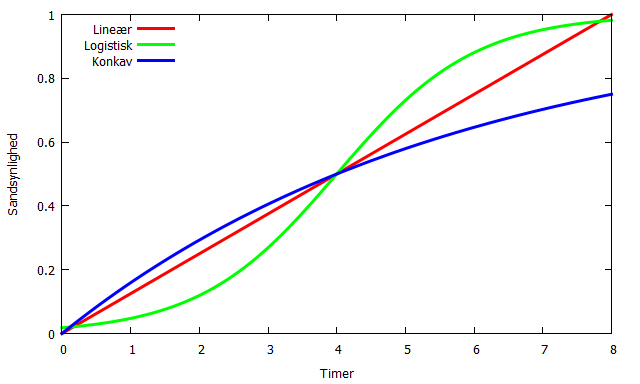
\includegraphics[scale=0.33]{graf-funktionseksempler}
	\caption{Tre funktioner til estimering af sandsynlighed for søvn}\label{fig:trefunc}
\end{figure}

\cref{fig:trefunc} viser tre forslag til en sådan funktion.
Disse er den røde lineære funktion, den blå konkave funktion og den grønne logistiske funktion \citep{wiki:LogisticFunction}.
Alle tre funktioner har til fælles at de er voksende, hvilket passer med vores antagelse af jo længere der har været stilstand jo større sandsynlighed er der for at man sover.
Den lineære funktion bygger på antagelsen, at sandsynligheden for at man sover er kongruent med stilstandslængden, hvilket vi ikke ønsker da vi så tillægger for stor vægt til korte stilstandsperioder. Imidlertid kan det godt være at den lineære og konkave funktion ville være bedre til at registrere korte søvnperioder midt om dagen.
Dette kræver videre arbejde men som en start benyttes den logistiske funktion, men kan nemt udskiftes.


Dn logistiske funktion beskriver hvordan at ved længere stilstandsperioder er der en forøget hældning i funktionen, indtil vi nærmer os lange stilstandsperioder hvor ekstra tid ikke giver en meget forøget sandsynlighed for søvn. 
Dette kan ses da den logistiske funktion vi har plottet går asymptotisk mod 1, svarende til 100\% sikkerhed for søvn.
I realiteten kan vi aldrig være 100\% sikker på søvn ved lang stilstand, da det kan være man har glemt sin smartphone hjemme mens man er på tur over en weekend, men hvis forudsætningen for at systemet fungerer er at man har sin smartphone i nærheden, regnes den logistiske funktion som et godt redskab til et søvnestimat.

Definitionen af den logistiske funktion er defineret som følger:
\begin{equation}
	f(t_{span}) = \frac{L}{1+e^{\,-k\cdot(t_{span} - t_{midtpunkt})}}
\end{equation} 
hvor,
\begin{itemize}
	\item[$L$] er kurvens maksimums værdi, hvilket for os eksempelvis kan være $1$ for 100\% sandsynlighed for at man sover.
	\item[$k$] er stejlheden for kurven.
	\item[$t_{span}$] Tidsperiode siden starten på stilstandsperioden målt i timer.
	\item[$t_{midtpunkt}$] Er det tidspunkt hvor kurven når $L/2$, hvilket i figurens tilfælde er hvornår kurven når $0.5$ det vil sige ved 4 timer.
\end{itemize}

Der kan argumenteres for en lavere værdi for $L$ så man maks kan blive 90\% sikker, men er noget der bør overvejes med mere træningsdata. 
Det kan også være en god idé at ændre på stejlheden for kurven, altså k, baseret på hvilken kilde af data man bruger som f.eks. accelerometer eller lyd.
Desuden skal $t_{midtpunkt}$ værdi på 4 timer betragtes som et første bud der passede fint med det observerede data, men kan justeres.

\subsection{Kombinering af modeller}\label{subsec:kombimodeller}
Det er tiltænkt at hver sensor kan have en tilknyttet søvnestimeringsmodel, hvilket i vores tilfælde er en søvnestimeringsmodel for accelerometret og en for amplituden.
Imidlertid kan det være en fordel at have en samlet model der kombinerer resultaterne fundet for de enkelte modeller.
En metode til dette er det vægtede gennemsnit og er et redskab vi har beskrevet i \cref{sec:redskaber}
Vores implementering af det vægtede gennemsnit afviger fra et normalt vægtet gennemsnit, idet at for de enkelte søvnestimeringsmoduler er der ikke blevet registreret data på samme tid eller i samme mængde.
På grund af dette tager modulet højde for hvis der er mangel på en estimering til en given tid for et af søvnestimeringsmodulerne.
Måden dette gøres er ved at tages den forrige værdi til estimeringen.
Man kan forestille sig en lynlås hvor der skiftes mellem takkerne fra hver del, på samme måde gøres med estimeringerne for hvert modul, for at illustrere dette bruges der et eksempel.

\newcommand{\nv}{Ingen estimering}

\begin{table}[h]
\centering
\resizebox{\columnwidth}{!}{\begin{tabular}{|c|c|c|p{2.5cm}|}
\hline Tid & Sandsynlighed for model A & Sandsynlighed for model B & Resultat\\ 
\thickhline 02:30:00 & 	0.59    & \nv  	& $\text{Vægt}_A * 0.59 + \text{Vægt}_B * 0.29$\\ 
\hline 02:30:01 & 	\nv     & 0.29 	& $\text{Vægt}_A * 0.61 + \text{Vægt}_B * 0.29$\\ 
\hline 02:30:02 & 	0.61    & \nv 	& $\text{Vægt}_A * 0.61 + \text{Vægt}_B * 0.30$\\
\hline 02:30:03 & 	0.62    & 0.30 	& $\text{Vægt}_A * 0.62 + \text{Vægt}_B * 0.30$\\ 
\hline 02:30:04 & 	0.63    & \nv 	& $\text{Vægt}_A * 0.63 + \text{Vægt}_B * 0.31$\\ 
\hline 02:30:05 & 	\nv     & 0.31 	& ...\\
\hline 
\end{tabular}} 
\caption{Tabel der illustrerer hvordan kombineringen fungerer. $\text{Vægt}_A$ og $\text{Vægt}_B$ er de fastsatte vægte for de to modeller.}
\label{tab:combiModelsExample}
\end{table}

I \cref{tab:combiModelsExample} kan man se kombineringen af de to modeller.
Måden den kombinerer sandsynligheder på er ved at den starter med to gennemløbere, henholdsvis for A og B, som starter på det første element som ikke er tom. 
Så derfor i eksemplet vil A starte ved 02:30:00 med værdien $0.59$ og for B vil den starte ved 02:30:01 med værdien $0.29$. 
Disse to værdier kombineres for det bagerste element med vægtningerne for de to modeller, hvorefter flyttes den bagerste gennemløber, og en ny kombinering foretages.
Dette forsætter indtil der ikke er mere data tilbage i en af de to gennemløbere, hvorefter der ventes på ny data så begge gennemløbere igen har data at køre på.

\subsection{Aggregering}\label{subsec:soevnaggre}
Som demonstreret giver søvnestimeringsmetoden, der er vist som proof of concept, en estimering til en lang række tidspunkter.
Men for at give et ekstra redskab til at danne et overblik over disse estimeringer, kan der med fordel som proof of concept laves en aggregering af søvnestimeringsdata.

For at få et bedre indblik i formen af data der skal aggregeres gives et eksempel i \cref{tab:noaggsoevndata}.
\begin{table}[h]
	\centering
\begin{tabular}{|c|c|c|}
	\hline {\_}id & prob & time \\ 
	\thickhline 203754 & 0.050 & 2015-04-26 01:41:42.446 \\ 
	\hline 203755 & 0.050 & 2015-04-25 01:41:43.375 \\ 
	\hline ... & ... & ... \\ 
	\hline 218777 & 0.919 & 2015-04-26 05:52:36.204 \\ 
	\hline 218778 & 0.919 & 2015-04-26 05:52:37.203 \\ 
	\hline 218779 & 0.000 & 2015-04-26 05:52:38.163 \\ 
	\hline 
\end{tabular}
\caption{Eksempel på søvnestimeringsdata, der ikke er aggregeret.}\label{tab:noaggsoevndata}
\end{table}
Ved at se på data som i \cref{tab:noaggsoevndata} fremstår det hvordan at fra {\_}id 203754 til {\_}id 218778 er sandsynligheden for søvn, der ses i \textit{prob} kolonnen, monotont voksende.
Idéen derudfra er så at registrere sådanne monotoniforhold og aggregere data med hensyn til det.
Det vil sige at registrere intervaller hvor \textit{prob} er tilpas stor over en længere tidsperiode, samt er monotont voksende.

Det blev besluttet at forkaste intervaller kortere end 10 minutter og hvor sandsynligheden for søvn i slutningen af intervallet er under 10\%.
Dette kan være en fornuftig løsning under antagelse af at man er rolig når man sover, og har da også vist gode resultater med nogle tests af personer med en meget rolig søvn. 
Eksempelvis med det viste data i \cref{tab:noaggsoevndata} vil dette blive aggregeret til en række som set i \cref{tab:aggdat}.

\begin{table}[h]
	\centering
\begin{tabular}{|c|c|c|c|}
	\hline {\_}id & startdate & enddate & prob \\ 
	\thickhline 1 & 2015-04-26 01:41:42.446 &  2015-04-26 05:52:37.203 & 0.919 \\ 
	\hline 
\end{tabular} 
\caption{Aggregering af data fra \cref{tab:noaggsoevndata}.}\label{tab:aggdat}
\end{table}

Vi har dog også fundet tilfælde hvor en aggregering ikke er akkurat, eksempelvis ved snorken fejler denne aggregering da den er for naiv, yderligere diskussion om hvad man kan gøre i stedet for er beskrevet tidligere i \cref{section:snorken}.
Et alternativ kunne være at tage arealet af søvnestimeringsdata, og bruge arealet som estimat til hvor meget man har sovet per dag.
Dette har ulempen at det ikke vil oplyse om selve søvnperioderne men blot mængde af søvn per dag, derudover vil den stadig blive påvirket af snorken og andre støjfaktorer.
Vi hæfter os ved at denne aggregeringsmetode er ment som et proof of concept og med ekstra ressourcer kan det være fornuftigt at se på andre aggregeringsmetoder og inddrage fundne snorken estimeringer til at kunne aggregere søvndata på mere akkurat vis. Forslag til dette kan læses i \cref{section:snorken}.

\subsection{Visualisering}\label{sec:pocVis}
For at kunne vise brugeren af systemet hvordan deres søvn har været, skal der tilføjes nogle visningsmoduler.
Disse visningsmoduler skal kunne give et overblik over hvordan man har sovet den seneste nat, men også hvordan man har sovet det seneste stykke tid.

For at kunne udtrykke dette til brugeren er der først blevet lavet en graf der viser hvor sikker systemet er på at man har sovet over en periode.
Denne periode er sat til at være alt data der er på smartphonen så brugeren har overblik over ændringer i grafen.
Disse ændringer kan derved indikere at der er sket en ændring i ens sindstilstand.
Til at sørge for at grafen kan bruges til både at se hvordan man har sovet over en længere periode samt over en kort periode, har man den mulighed at man kan zoome på grafen, og derved se præcis hvor sikker systemet er på man har sovet på et bestemt tidspunkt.
Der er også lavet en graf for hvor sikker systemet ved hjælp af kun acceleration er på at man sover, det samme gælder for lyd, se \cref{fig:visningsgrafer}.

\begin{figure}[h]
	\centering
	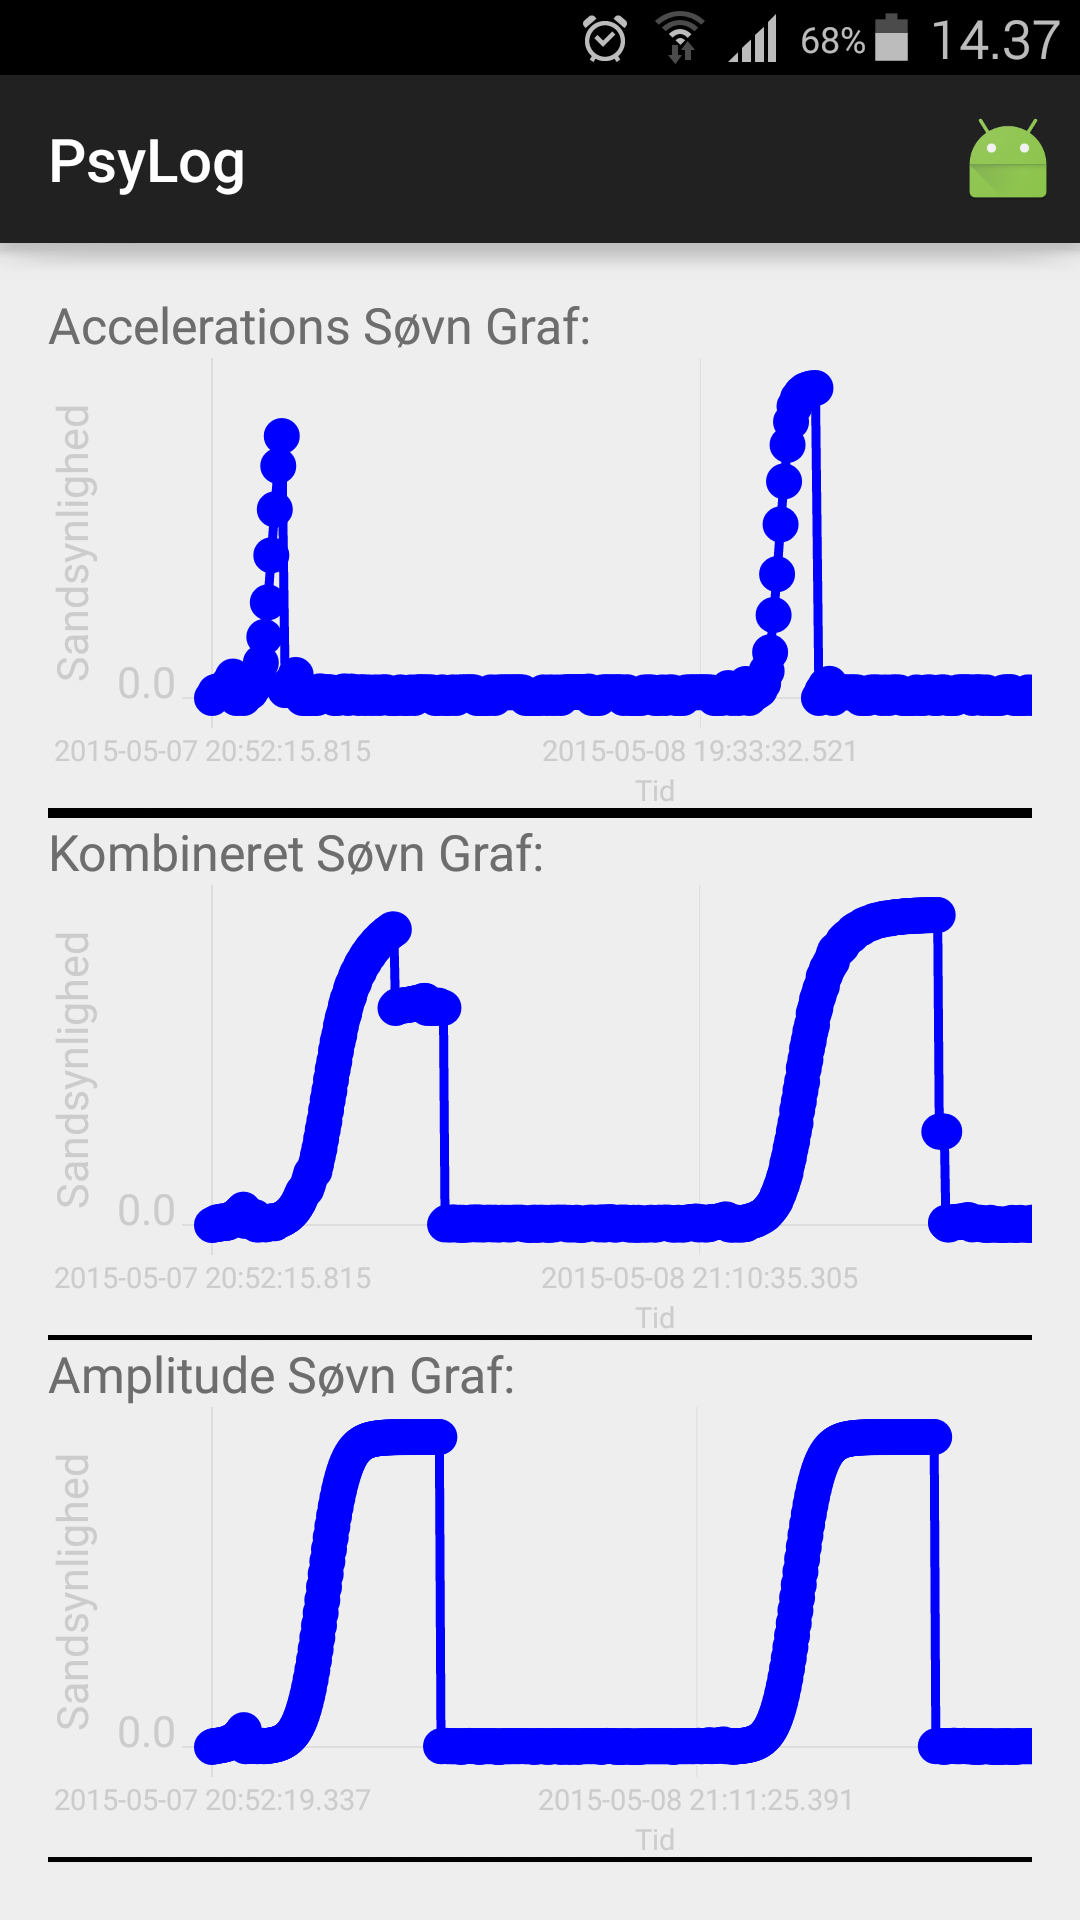
\includegraphics[scale=0.1]{visningsgrafer}
	\caption{Tre funktioner til estimering af sandsynlighed for søvn}\label{fig:visningsgrafer}
\end{figure}

Grafer er dog ikke altid lige nemme at forstå, derfor er der blevet lavet en tabel der viser hvor sikker systemet er på at man har sovet over en periode.
Denne tabel minder om den der blev vist i \cref{tab:aggdat}, dog uden $\_id$ kolonnen.
Tabellen giver et nemt overblik for brugeren om hvornår man har sovet, samt hvor sikker systemet er på at man har sovet.
Dog er det ikke så nemt for brugeren at se ens adfærdsændring i en sådan tabel, da det kræver at man kigger på meget data på en gang.
Som alternativ kan der ses på et 'early warning modul', og er diskuteret i \cref{chap:bigdisc}.
% Giv eksempel på ikke aggregeret data.
% Forklar forslag/løsning til aggregering af data.
% Vis resultat derfor
% Diskuter problemer? (e.g. snorken) evt. referer til snorken diskussion
\section{Videre Arbejde}\label{sec:videre-arbejde-fa}
Denne sektion detaljerer forskellige ting som kunne arbejdes videre på ved aktivitet.
Idet at der ikke har været en stor fokus på fysisk aktivitet, er det idéelt at arbejde videre på.

\subsection{Fra Skridt til Aktivitet}
Den nuværende funktionalitet til fysisk aktivitet er kun en skridttæller, fra denne vil det næste logiske skridt være at lave noget der kan give et overblik over hvor meget fysisk aktivitet der har været ud fra antallet af skridt.
Helt præcist hvordan dette skal gøres og vises er uvist, men der er en mulighed for at det skulle kombineres med accelerometer data til at afgøre om der er tale om løb, gang eller anden form for bevægelse.
De forskellige gang typer skulle så også fortolkes som forskellige grad af aktivitet. 
Det ville også være nødvendigt at beslutte hvad for en enhed fysisk aktivitet er i, er det i Joule forbrændt eller noget andet?

Udover at beslutte hvordan fysisk aktivitet skal bestemmes skal man også beslutte sig for hvad det skal bruges til.
I sammenhæng med det primære fokus vi har på affektive lidelser, vil et oplagt fokus være at se på ændringer i mængden af fysisk aktivitet, da det giver et signal om ændringer i sindstilstand for patienter med affektive lidelser, hvilket også blev nævnt i \citet[Kapitel 1, Sektion 4]{misc:faellesrapp}.

\ivan{Lidt tyndt om opgørelse af aktivitet over tid, trendanalyse o.lign.}
\subsection{Sammenhæng Mellem Søvn og Aktivitet}
Som nævnt i starten af dette kapitel, har vi en teori om, at der kunne være en sammenhæng mellem folks søvnkvalitet og deres bevægelsesmønster.
Teorien bør undersøges, både i den forstand at man skal undersøge om det er noget andre folk har overvejet, og undersøge om det er muligt at indsamle tilstrækkeligt data på en mobil enhed til at komme med noget brugbart omkring dette.

Derudover bygger teorien på en antagelsen at dårlig søvn har en påvirkning på aktivitets niveau.
For eksempel kunne en person som har sovet dårligt være mere tilbøjelig til at slæbe sine fødder end en veludhvilet person vil.
Vi er af den overbevisning at dette sagtens kunne være tilfældet, men på samme tid vil det være en god idé at finde noget der underbygger det.

\subsection{Andre Former for Aktivitets Målinger}
Indtil videre er der kun blevet lavet aktivitets udregninger ved hjælp af en skridttæller, idet at meget fysisk aktivitet vil tælle som skridt, såsom cykling og løb. 
Men der er er andre former for fysisk aktivitet hvor det sandsynligvis ikke vil fungerer specielt godt, for eksempel træning i et trænings center hvor der er tale om forskellige former for vægtløftning. 
Det kan godt være at skridttælleren vil fungerer delvist til dette, men den vil ikke kunne få hele billedet.

Sådanne former for fysisk aktivitet bliver ikke dækket af en skridttæller og er formodentlig umulig at detektere via en telefon, for ikke at nævne at mange folk muligvis ikke har deres telefon på sig når de træner i et trænings center.
Derfor vil registrering af andre former for fysisk aktivitet kræve ekstra udstyr udover smartphone, sandsynligvis et smartwatch eller smartwristband.

Der er dog en hvis sandsynlighed for at denne form for aktivitets registrering ikke er relevant for flertallet af patienter med affektive lidelser, da det kan være disse ikke går i træningscentre og træner, men dette vides ikke med sikkerhed.

De teknologier der kunne overvejes til fysisk aktivitet i et trænings center, kunne også give et bedre billede af fysisk aktivitet udenfor træningscenteret, da disse vil have adgang til ting som puls måling og galvanisk hud respons ved siden af det accelerometer data telefonen har til rådighed.
Derfor kunne tilføjelsen af supplerende datakilder muligvis give en bedre beskrivelse af fysisk aktivitet.

\chapter{Diskussion}\label{chap:bigdisc}
Søvn- og fysisk aktivitets-moduler er blevet præsenteret, og en diskussion om videre arbejde ved hver af disse kan læses i henholdsvis \cref{sec:videre-arbejde} og \cref{sec:videre-arbejde-fa}.
Imidlertid er der en række udfordringer som er fælles for hele løsningen der kræver opmærksomhed, og lyder som følger:
\begin{itemize}
	\item Hvordan kan registrering af fysisk aktivitet og søvn komplementere hinanden?
	\item Ændring i adfærd.
	\item Videre arbejde angående visualisering.
	\item Plads og performance problemer.
\end{itemize}

% Fysisk aktivitet og søvn komplement
Idéen ved at have søvn og fysisk aktivitet er at dække både når der soves og når man er vågen.
Hvis man kan dække hele dagen har vi mulighed for at logge patientens adfærd døgnet rundt.
Arbejdet består så i at udnytte denne dækning af døgnet.
Med den nuværende implementering er der udviklet moduler til at estimere antal skridt samt længden på søvn.
Disse kan udvikles videre, men på et tidspunkt med nok videre arbejde vil man have nogle relativt akkurate moduler.

% Ændring i adfærd.
Opgaven går derefter på at registrere ændring i adfærd. 
Registrering af ændring i adfærd er blevet understreget som helt centralt hvad angår forebyggelse for patienter med affektive lidelser \citep[1.4, Møde med Psykiatri professor Jørgen Aagaard]{misc:faellesrapp}.
En idé til systemet er at implementere et 'early warning modul', altså at personer med affektive lidelser vil bruge systemet og de vil blive notificeret om ændring i adfærd, hvorefter de så kan reagere derpå. 
Registrering af ændring i adfærd er imidlertid ikke blevet arbejdet på, da som forudsætning for at vi kan lave denne registrering bliver vi nødt til at have akkurate analysemoduler.
Det er derfor blevet udeladt, men er noget der skal blive arbejdet videre på når analysemodulerne har nået et tilpas modent stadie.

% visualisering
Efter analysemodulerne er blevet tilpas modne, lyder opgaven også på at visualisere data.
Det er tiltænkt at visualiseringerne skal være nemme at forstå og give et overblik over situationen, som også er nævnt af Jørgen Aagaard \citep[1.4, Møde med Psykiatri professor Jørgen Aagaard{misc:faellesrapp}. 
Derfor skal det undersøges hvordan man visualiserer data på en let-tilgængelig måde, hvor de fleste kan forstå hvad der foregår. 
Hvis det ikke er let at forstå, risikerer vi at de tiltænkte brugere af systemet ikke vil kunne forstå den indsamlede information.
På projektets nuværende stadie er dette ikke blevet undersøgt i detalje, som også kan læses om i \cref{sec:pocVis}, \cref{sec:soevnVisVidArb} og \cref{sec:aktivitetVis}. 
Derfor hæfter vi os ved at visualisering er vigtigt for brug af systemet, hvilket bør arbejdes videre med.

% Data beholdning, aggregrering, komprimering
Idet visualisering skal undersøges før systemet kan ses som komplet, er det også vigtigt at se på hvordan data opbevares idet at dette kan give problemer når det kommer til visualisering. 
Eksempelvis ved visualisering af store mængder data, kan dette give performance problemer, hvor man udsætter brugeren for en urimelig lang ventetid før visualiseringen kan præsenteres. 
Den store mængde af data kan også forårsage plads problemer. 
Af den grund er lagring i skyen samt aggregering og komprimering af data nødvendigt at undersøge.
Platformen er udviklet til at være modulær og fleksibel, hvorfor denne modificering ikke regnes for et større problem at udvikle.
Dermed er det ikke sagt, at det ikke vil være tidskrævende at udvikle, men platformen regnes for ikke at ville spænde ben for en sådan løsning.
Pladsforbrug er også set på som del af et eksperiment til PsyLog systemet, der skal undersøge hvor meget plads ikke-komprimeret og ikke-aggregeret data ville fylde, se \citet[3.4 Pladsforbrug eksperimenter]{misc:faellesrapp} for flere detaljer vedrørende dette.

Alt dette understreger at der er udfordringer man skal have i mente, og bør løses ved videre arbejde.

\chapter{Konklusion}
Afslutningsvis kan vi konkludere at vi har fået et indblik i løsninger til søvn- og fysisk aktivitetsestimering.
Dog må vi erkende at det er et stort emne der kræver mere arbejde.
Den nuværende løsning skal ses som et spadestik i et længere udviklingsforløb, men skaber et grundlag for videre arbejde med emnet.
Derudover skal de omtalte moduler ses som enkelte moduler i den større PsyLog software pakke.
I den sammenhæng kan andre moduler udvikles til at supplere den udviklede analyse, men kan også være andre moduler der kan estimere i andre henseender, eksempelvis søvnkvalitet.


Men selvom der havde været mere tid til arbejdet, anses det at dette domæne altid kan videreudvikles.
Med dette tænkes, at der i fremtiden med stor sandsynlighed vil komme nye metoder til estimeringen samt nyt teknologisk udstyr, der kan give nye datakilder man bør betragte.
Problemets natur er at man aldrig kan finde en færdig løsning, hvorfor platformen da også er udviklet med dette i tankerne.
Dermed ikke sagt at en tilstrækkelig løsning ikke kan findes, men blot at løsningen altid ville kunne forbedres.

Vi kan konkludere at et proof of concept til estimering af søvn og fysisk aktivitet er udviklet, men disse løsninger er ikke færdige og bør forbedres ved videre arbejde.

Vores proof of concept løsning gør det dog nemmere at arbejde videre på søvnestimering.
Vi har opsat en primitiv måde at estimere søvn og fysisk aktivitet på, men det bygger ud fra en platform der er fleksibel og modular.
Denne tankegang følges også ved vores estimeringsmoduler, hvorfor det vurderes at dele af estimeringsmodulerne nemt kan udskiftes.
Eksempelvis kan den omtalte logistiske funktion nemt blive udskiftet til en anden metode.
Endvidere, er vores vurdering af stilstand op til debat, men er blot en måde at vurdere stilstand på og er i en separat metode og kan derfor også nemt udskiftes. 
Til sidst, som nævnt, kan de omtalte parametre også justeres, til at sikre en højere modenhed af estimeringsmodulerne.

%Vurdering af perspektiverne for denne slags teknologier inden for psykiatrien.


Det vurderes at når vores proof of concepts har nået en tilpas modenhed, hvilket er afgjort med den beskrevne verificering, kan det tages i brug i psykiatrien, til at give patienten indsigt i deres søvn og fysisk aktivitet. 
Ud fra samtaler med patienterne beskrevet i \citet{misc:faellesrapp}, fik vi det indtryk at de var åbne for brugen af et sådant system, i deres øjne var enhver ny metode velkommen.
Der forestilles at patienter bruger det udviklede system til at få overblik over deres fysiske aktivitet og søvn, og ved indikation på forværring af dette vil de kunne søge hjælp. 
Dette er knyttet til den omtalte trendanalyse der bør udvikles, og ville tage brug af de udviklede estimeringsmoduler.
Ved at have en sådan trendanalyse, giver det patienten mulighed for at blive opmærksom på ændring i adfærd, og kan være en nyttig ekstra hjælp til patienten.
Man skal dog være opmærksom på, at når sådanne produkter udvikles til brug inden for psykiatrien, har man med skrøbelige patienter at gøre.
Af den grund er det yderst vigtigt, at et sådant system ikke kan forårsage forværring for patienterne.
Det er af samme grund at systemet er blevet udviklet til at være oplysende fremfor dømmende, men systemet bør alligevel godkendes af psykiatrien inden det bør tages i brug af patienterne.

%Vurdering af perspektiver uden for psykiatrien (almen brug)
Systemet har også perspektiver uden for psykiatrien.
På nuværende stadie kan produktet også bruges til almen brug som en søvnestimerings eller fysisk aktivitetsestimerings applikation.
Man kan forestille sig at de udviklede estimeringsmoduler bruges i forskellige kontekster, hvor man vil på platformen knytte trendanalyse moduler på for patienterne, men hvor man kan nøjes med estimeringsmodulerne ved almen brug.
Løsningen ses altså ikke begrænset til psykiatrien men kunne også bruges til almen brug.

% Stort emne
% Fysisk aktivitet og søvn analyse kan lade sig gøre
% kræver mere arbejde
% Blive del af større software pakke (PsyLog)
% Ikke færdigt - men danner et grundlag for en mere komplet løsning
% Problemets natur gør at man aldrig er færdig - men har også været en tankegang der er fulgt i udviklingen (fleksibilitet - modularitet)


\bibliographystyle{unsrtnat}
\bibliography{Bibliography}
\label{bib:mybiblio}

\appendix
\chapter{Kode}
Til søvnestimeringen og fysisk aktivitet er der udviklet en række moduler.
Derudover er der lavet et udkast til hvordan visualiseringer skal se ud i PsyLog.
Links til de forskellige implementeringer kan findes herunder.

\begin{description}[style=nextline]
	\item[PsyLog - Viewbranch] \url{https://github.com/SW807/PsyLog/tree/e9e3b0e}
	\item[AccelerationSleepAnalysis] \url{https://github.com/SW807/AccelerationSleepAnalysis/tree/4e45b5f}
	\item[SoundSleepAnalysis] \url{https://github.com/SW807/SoundSleepAnalysis/tree/1426d23}
	\item[module-sleepstationary] \url{https://github.com/SW807/module-sleepstationary/tree/1aa3364}
	\item[module-sleepaggregator] \url{https://github.com/SW807/module-sleepaggregator/tree/bed463c}
	\item[module-stepcounter] \url{https://github.com/SW807/module-stepcounter/tree/20869e2}
	\item[module-stepcountaggregator] \url{https://github.com/SW807/module-stepcountaggregator/tree/66f9c69}
\end{description}

\end{document}